\documentclass[11pt]{article}

% \usepackage[UTF8]{ctex} % for Chinese 

\usepackage{setspace}
\usepackage[colorlinks,linkcolor=blue,anchorcolor=red,citecolor=black]{hyperref}
\usepackage{lineno}
\usepackage{booktabs}
\usepackage{graphicx}
\usepackage{float}
\usepackage{floatrow}
\usepackage{subfigure}
\usepackage{caption}
\usepackage{subcaption}
\usepackage{geometry}
\usepackage{multirow}
\usepackage{longtable}
\usepackage{lscape}
\usepackage{booktabs}
\usepackage{natbib}
\usepackage{natbibspacing}
\usepackage[toc,page]{appendix}
\usepackage{makecell}

\title{Graduate Trip for Master's Programme at Silwood, Imperial College \newline Day 1: Liverpool}
\date{2021.9.25}

\linespread{1.5}
\geometry{left=2cm,right=2cm,top=2cm,bottom=2cm}

\begin{document}

  \maketitle
  
  \newpage

  \linenumbers

\begin{figure}[H]
    \centering
    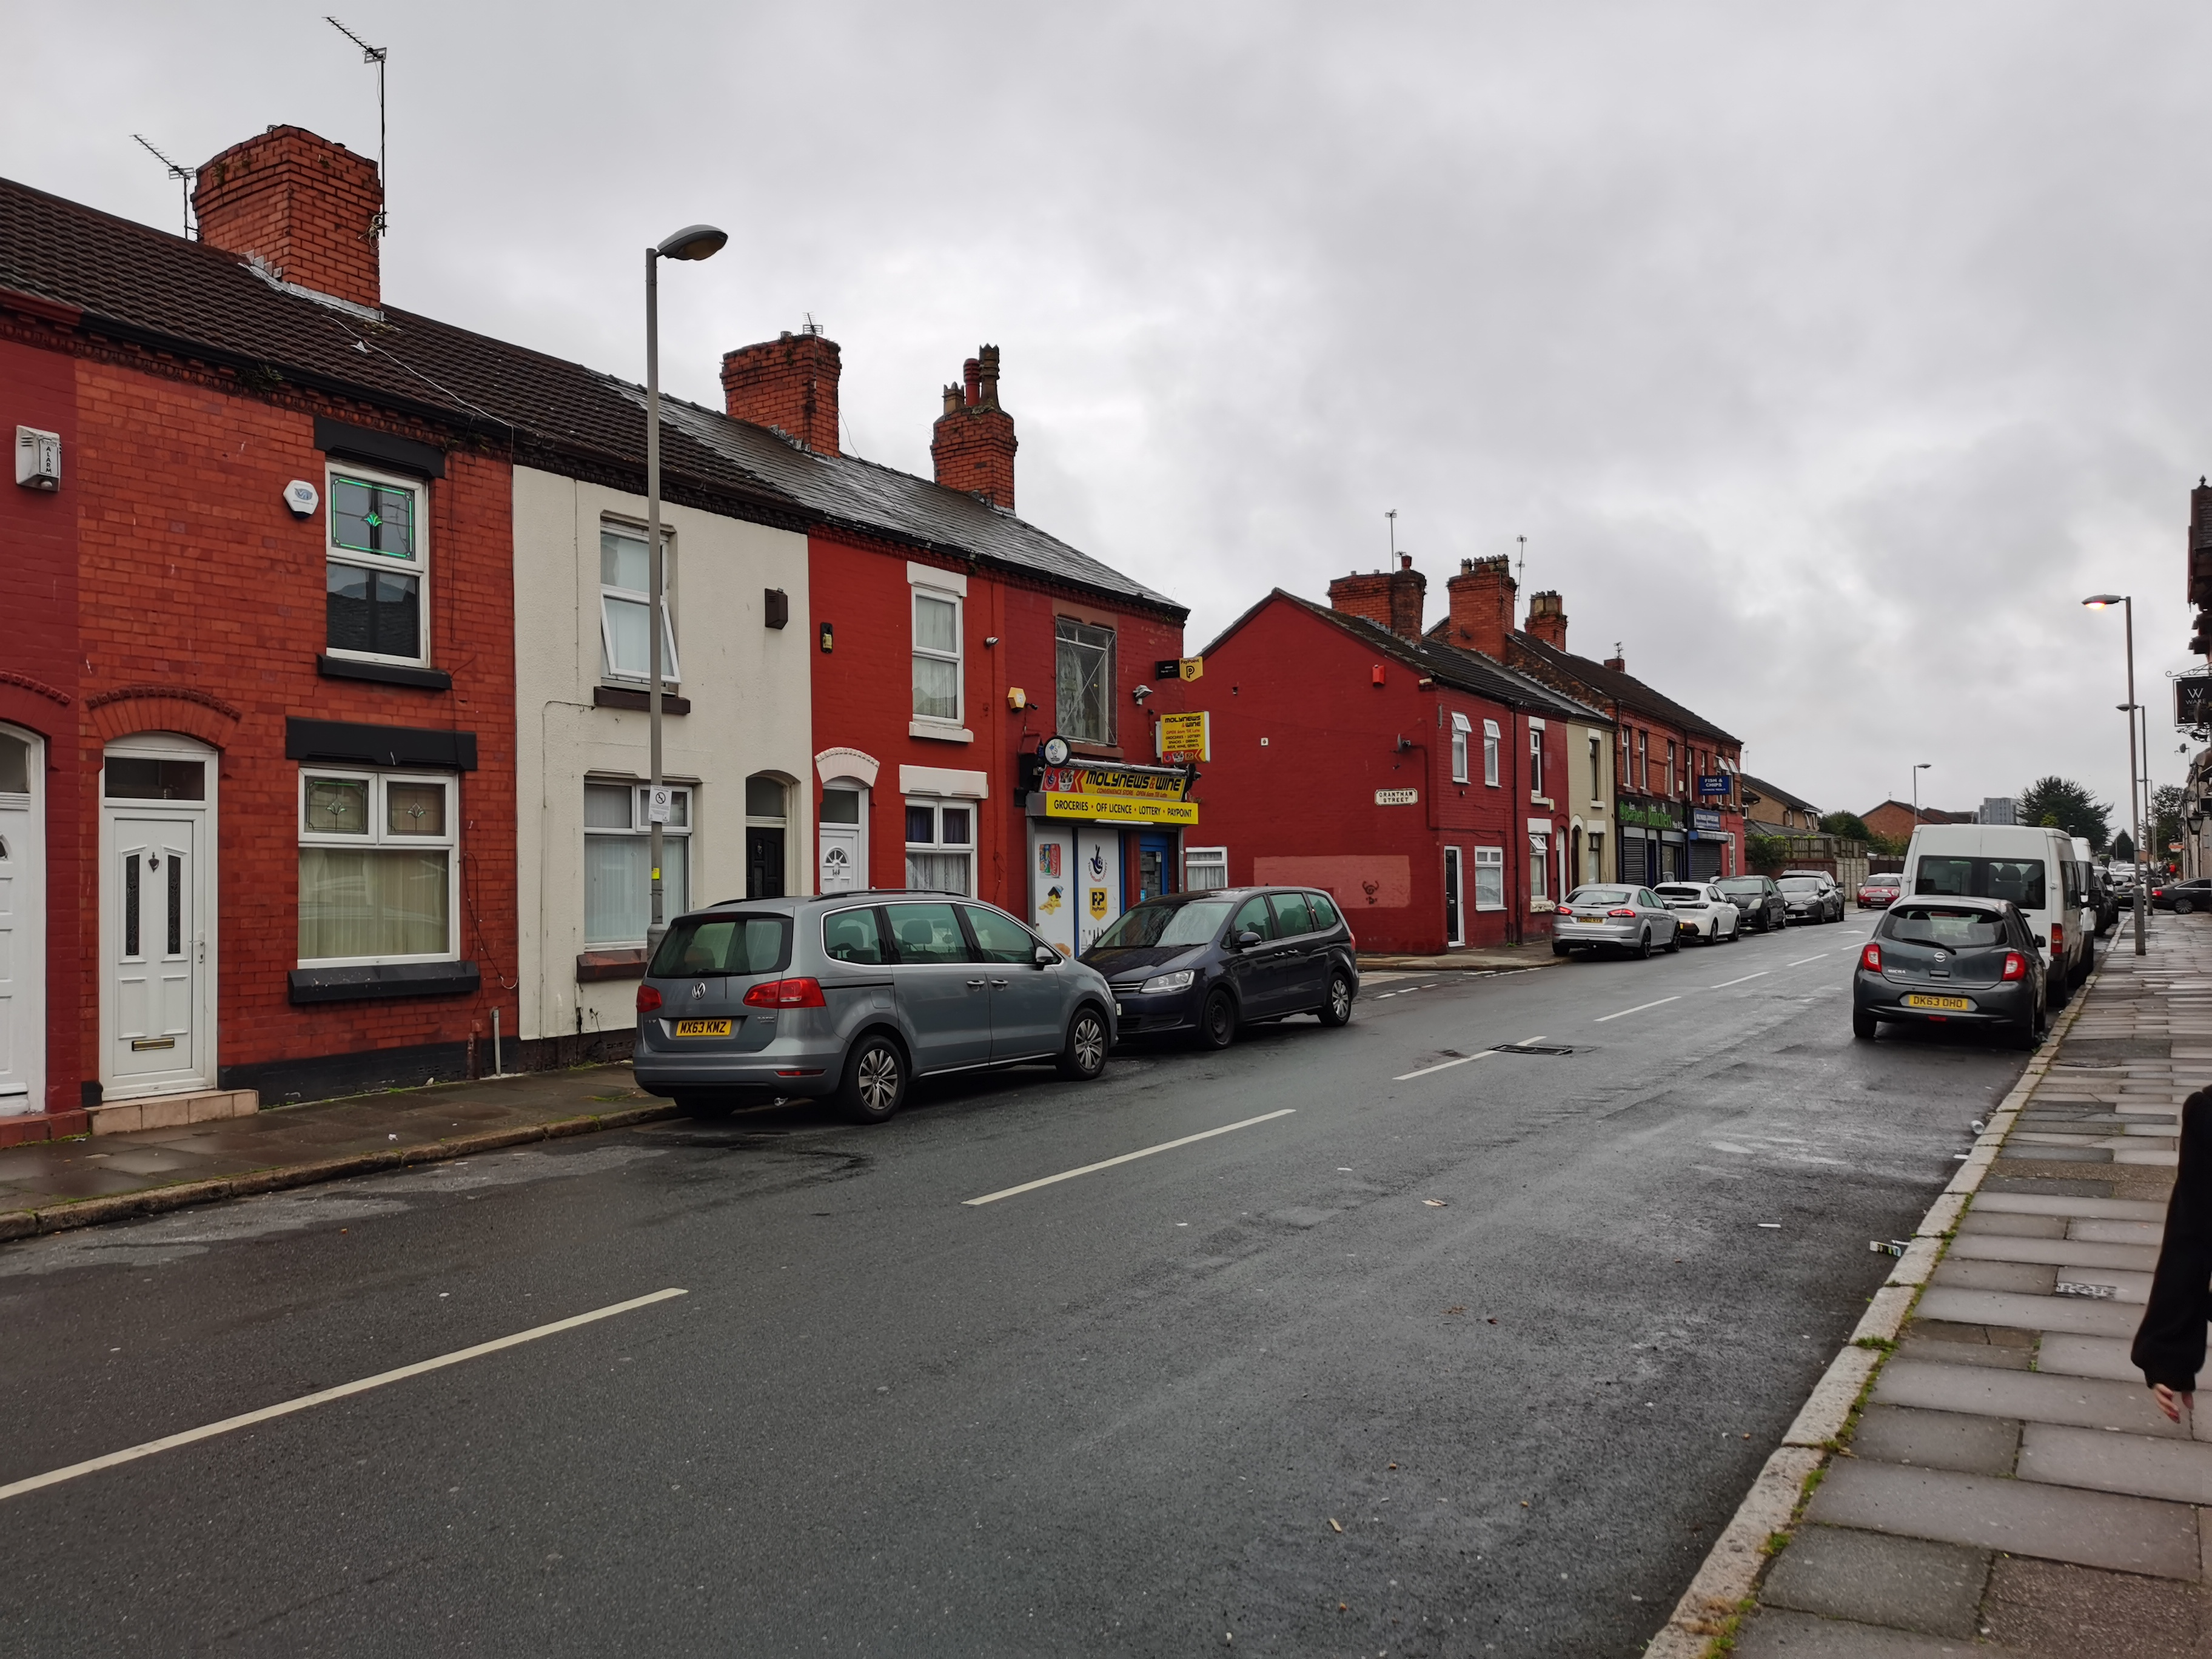
\includegraphics[width=\textwidth]{1A.jpg}
\end{figure}

\begin{figure}[H]
    \centering
    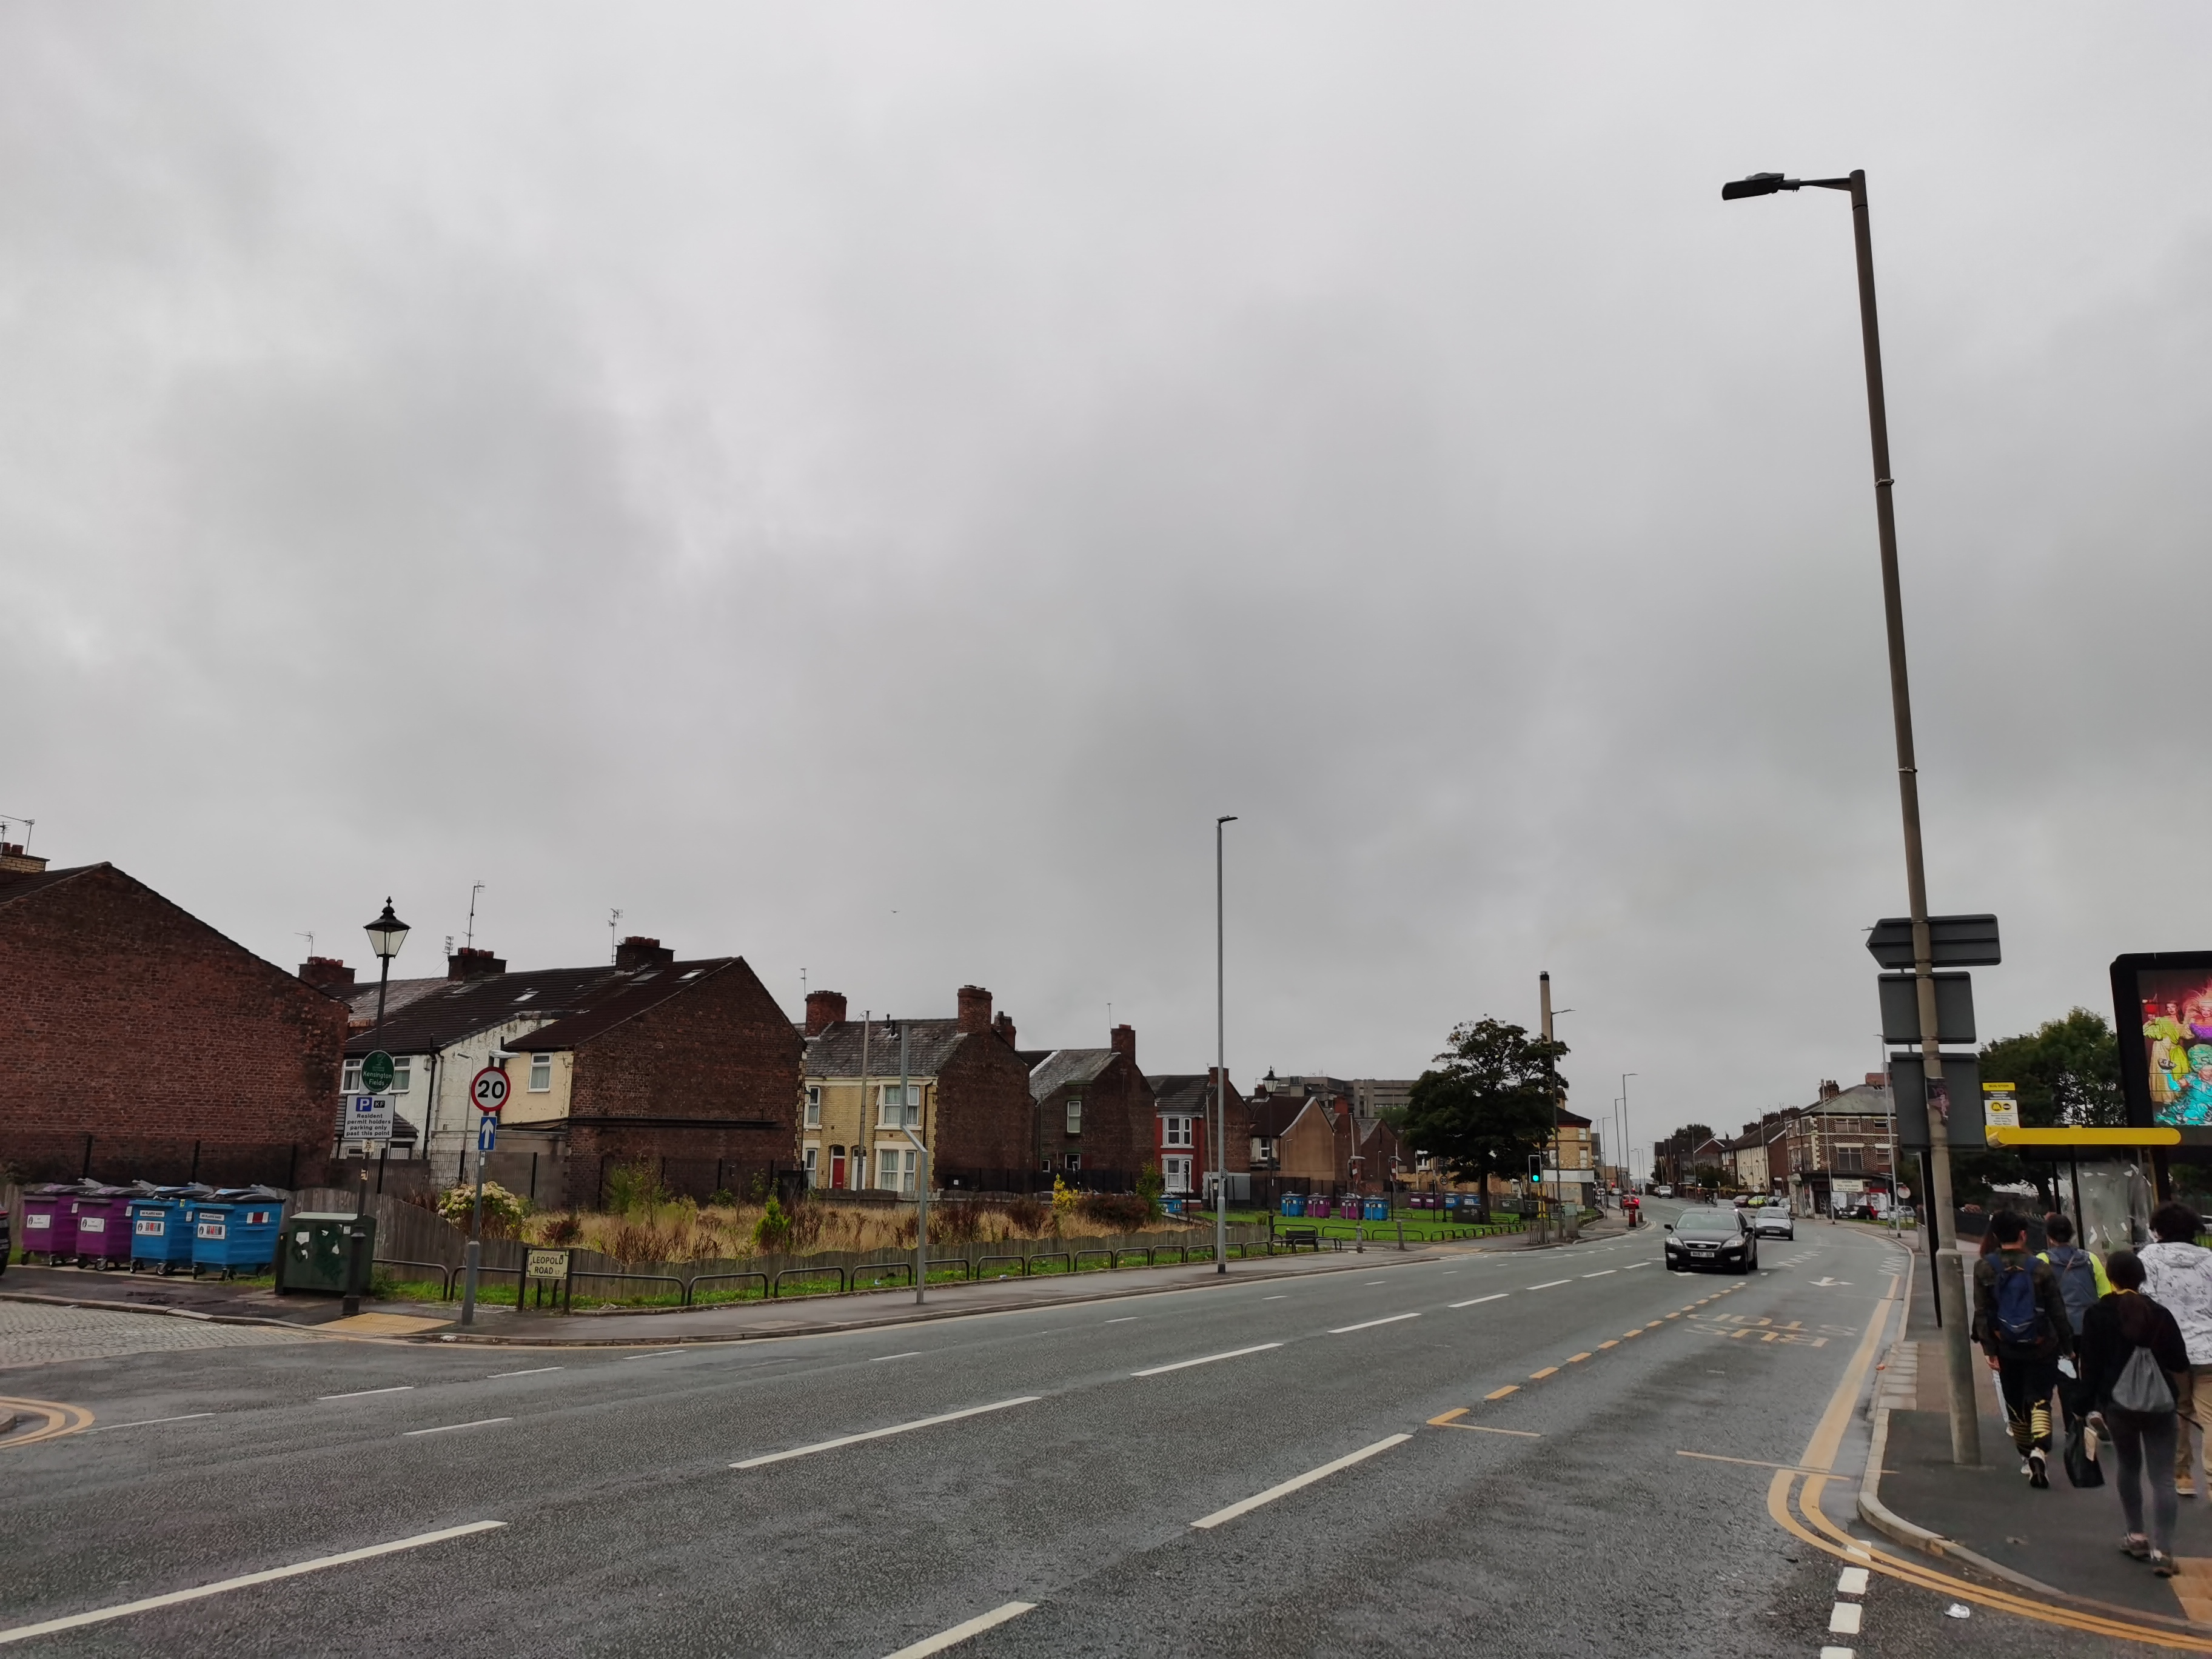
\includegraphics[width=\textwidth]{1B.jpg}
\end{figure}

\begin{figure}[H]
    \centering
    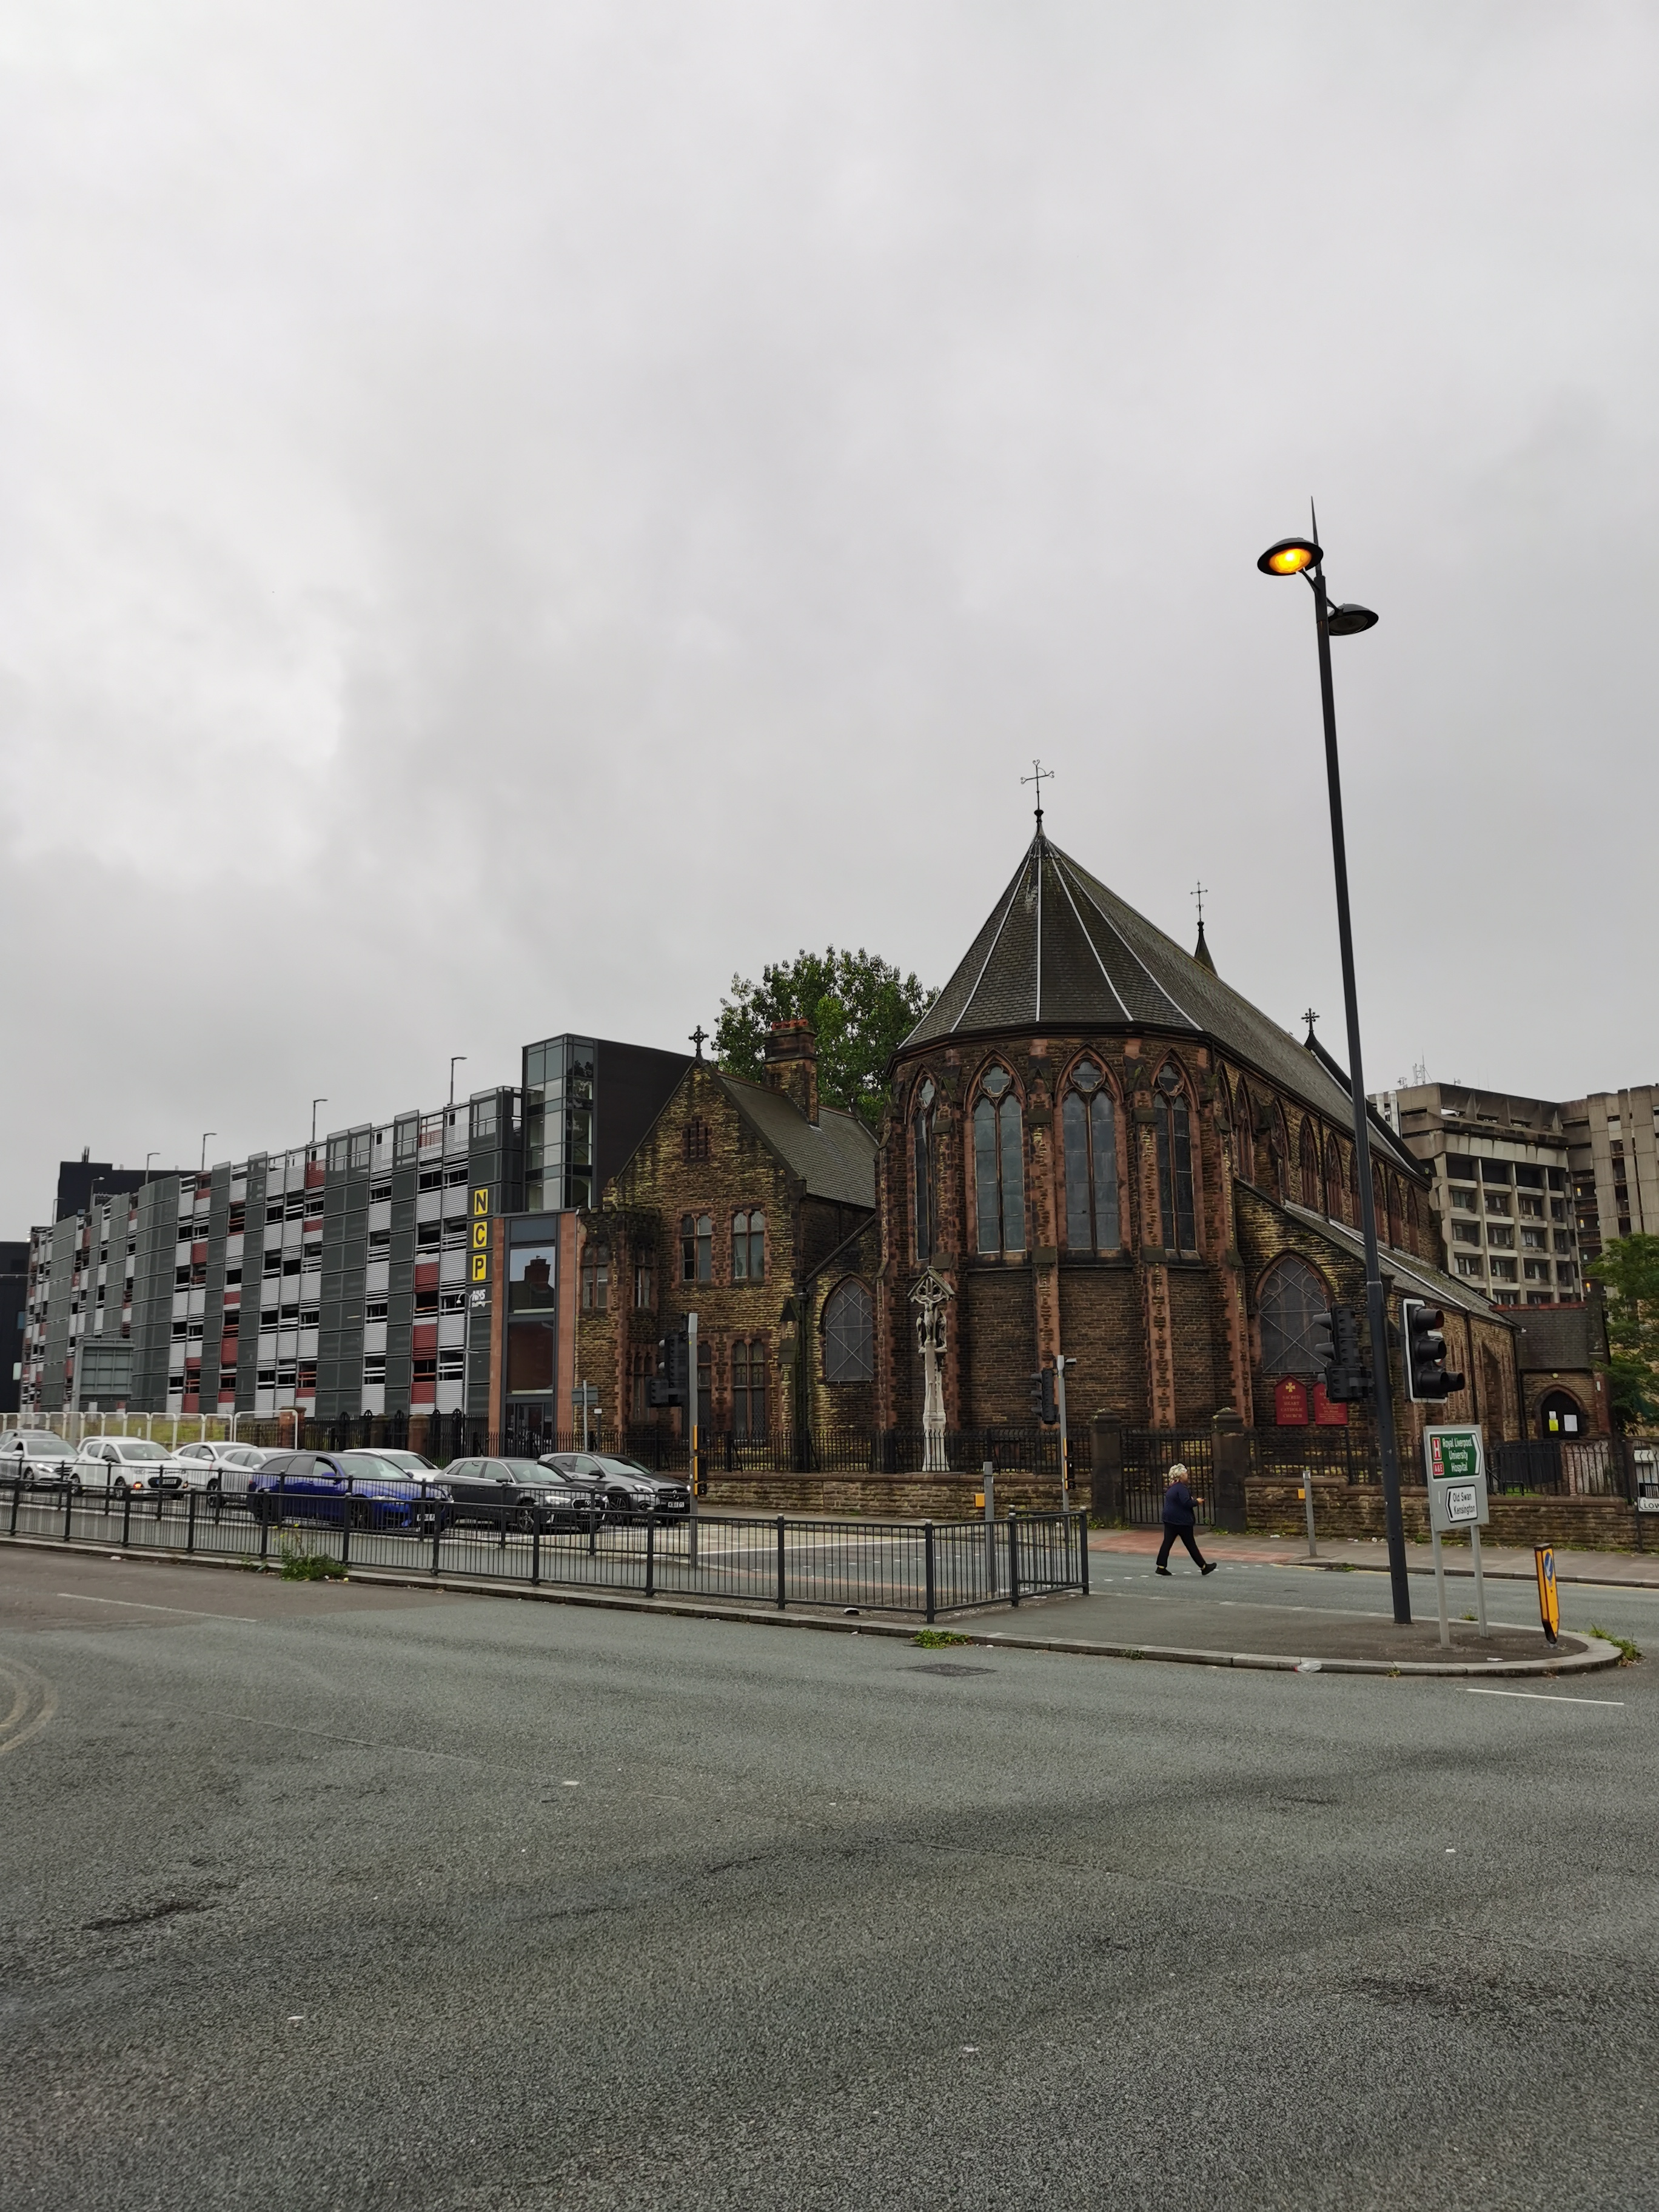
\includegraphics[width=\textwidth]{1C.jpg}
\end{figure}

\begin{figure}[H]
    \centering
    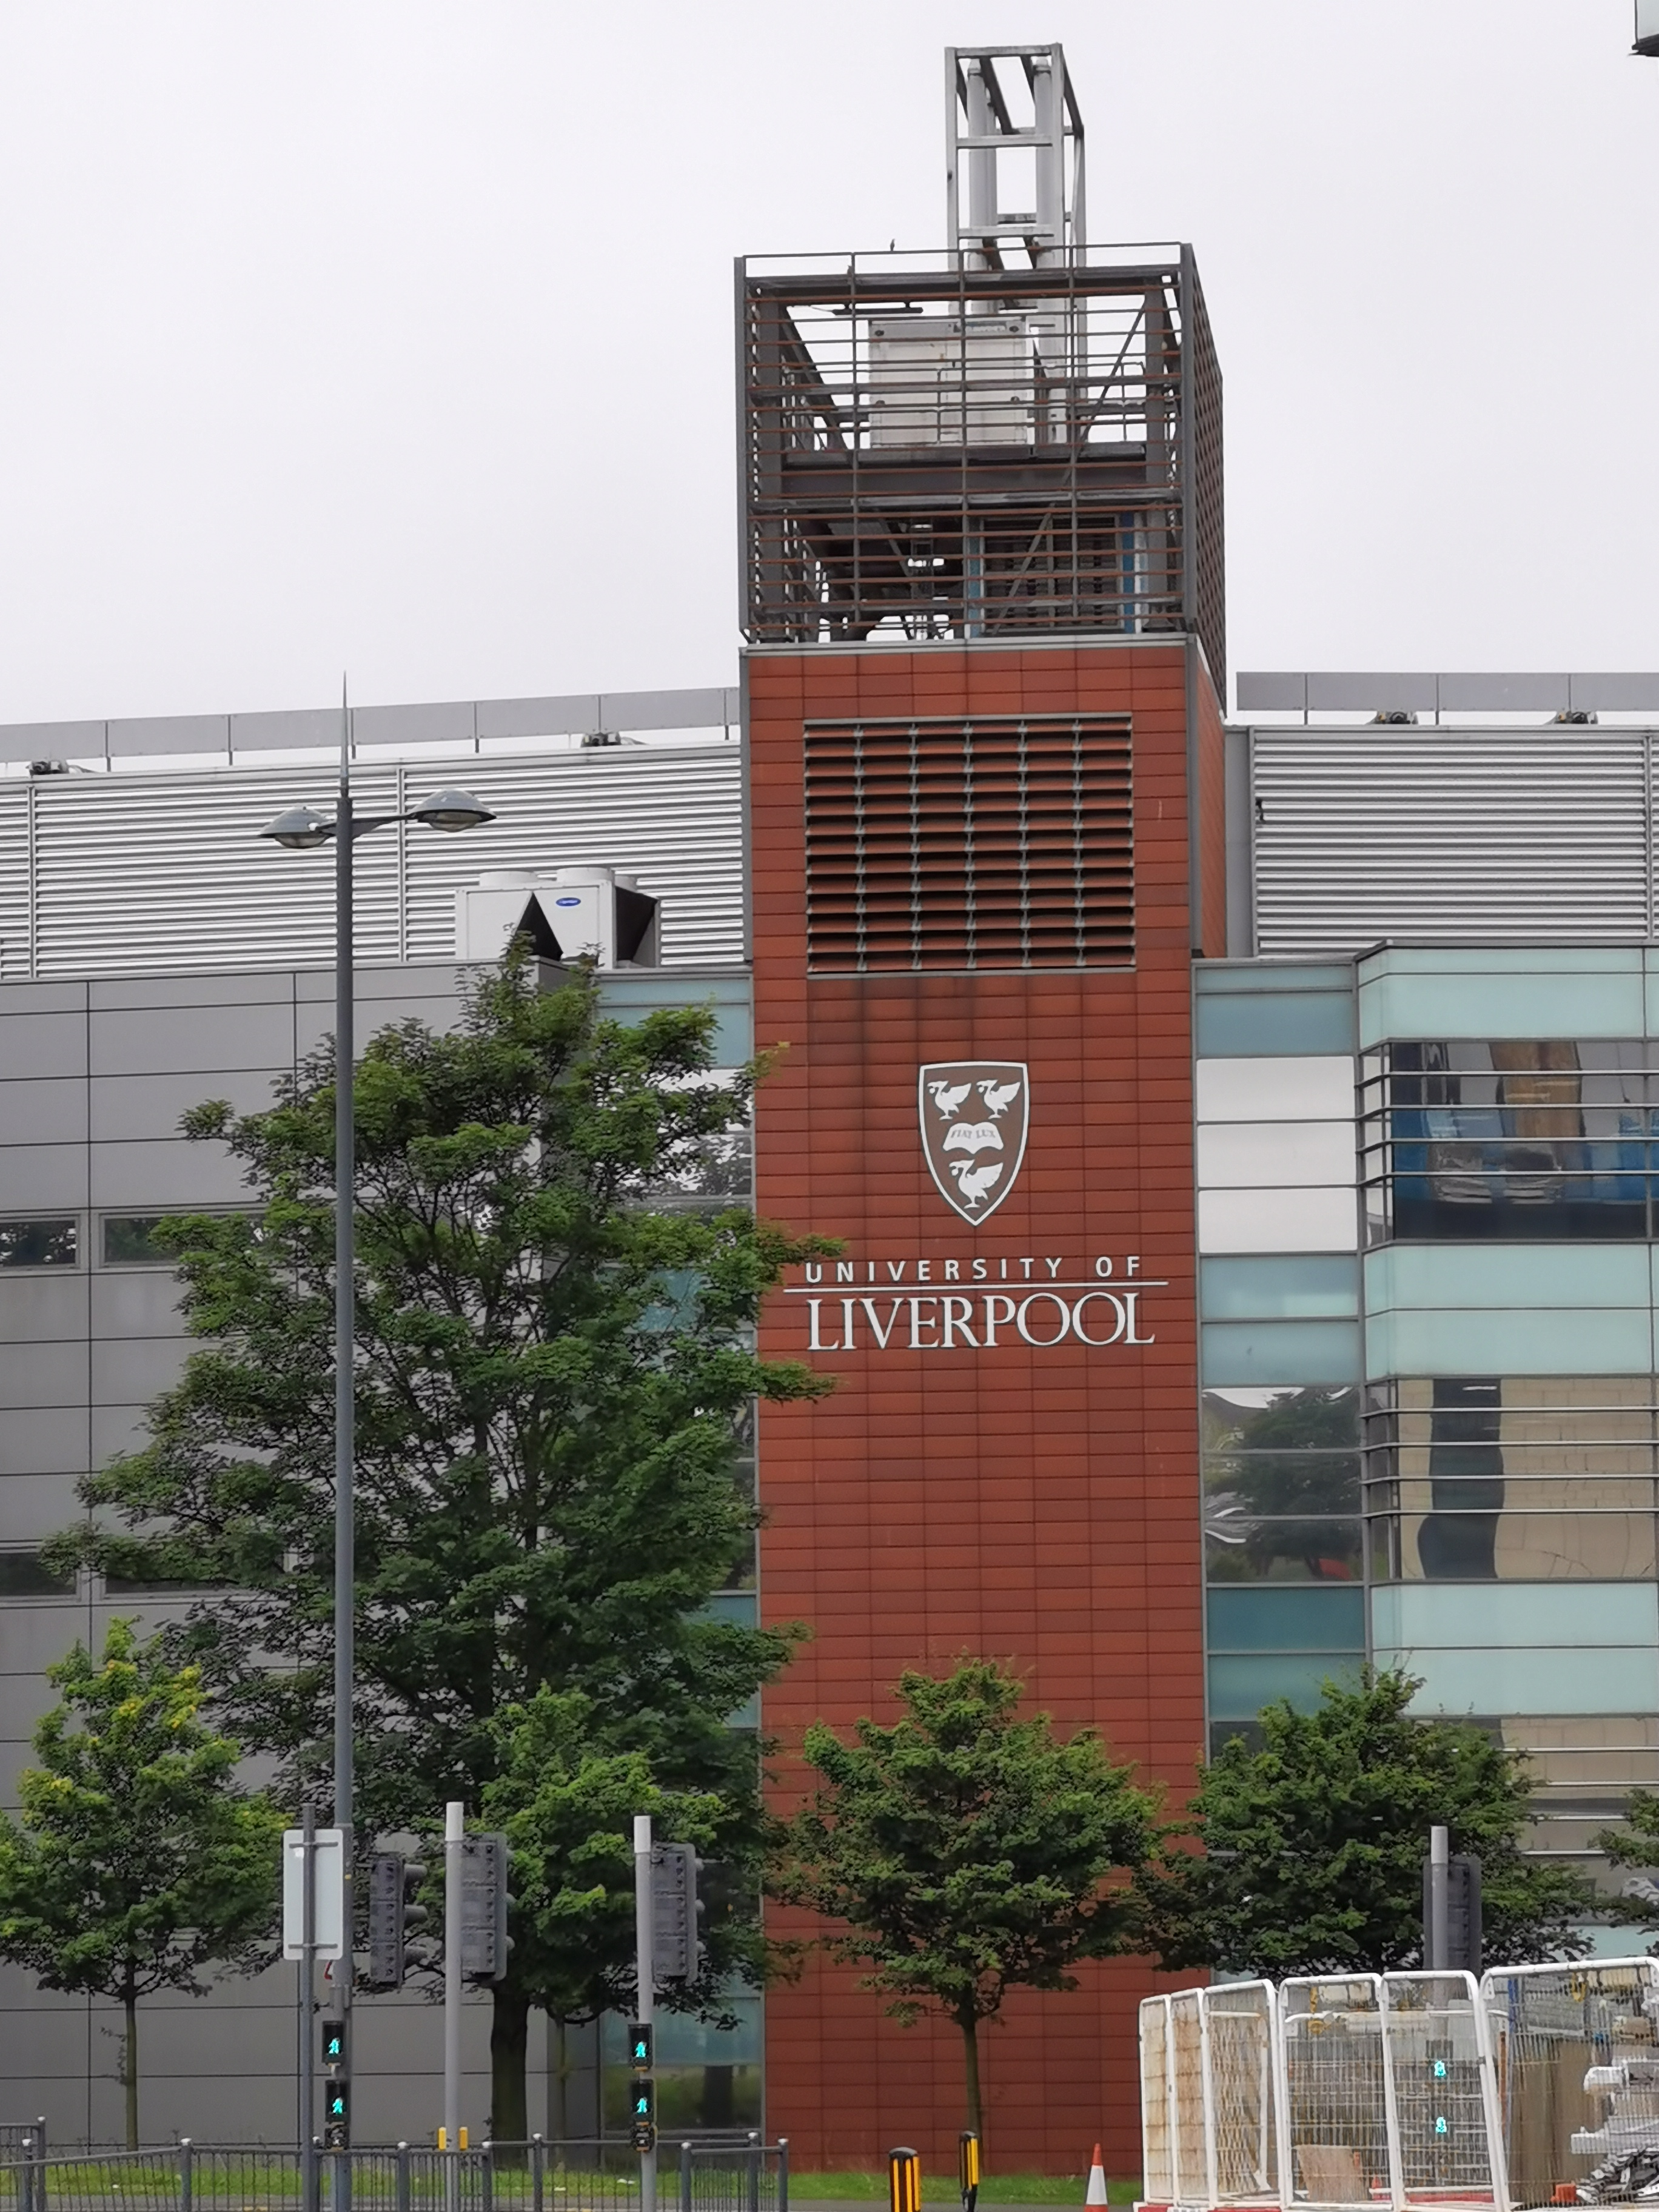
\includegraphics[width=\textwidth]{1D.jpg}
\end{figure}

\begin{figure}[H]
    \centering
    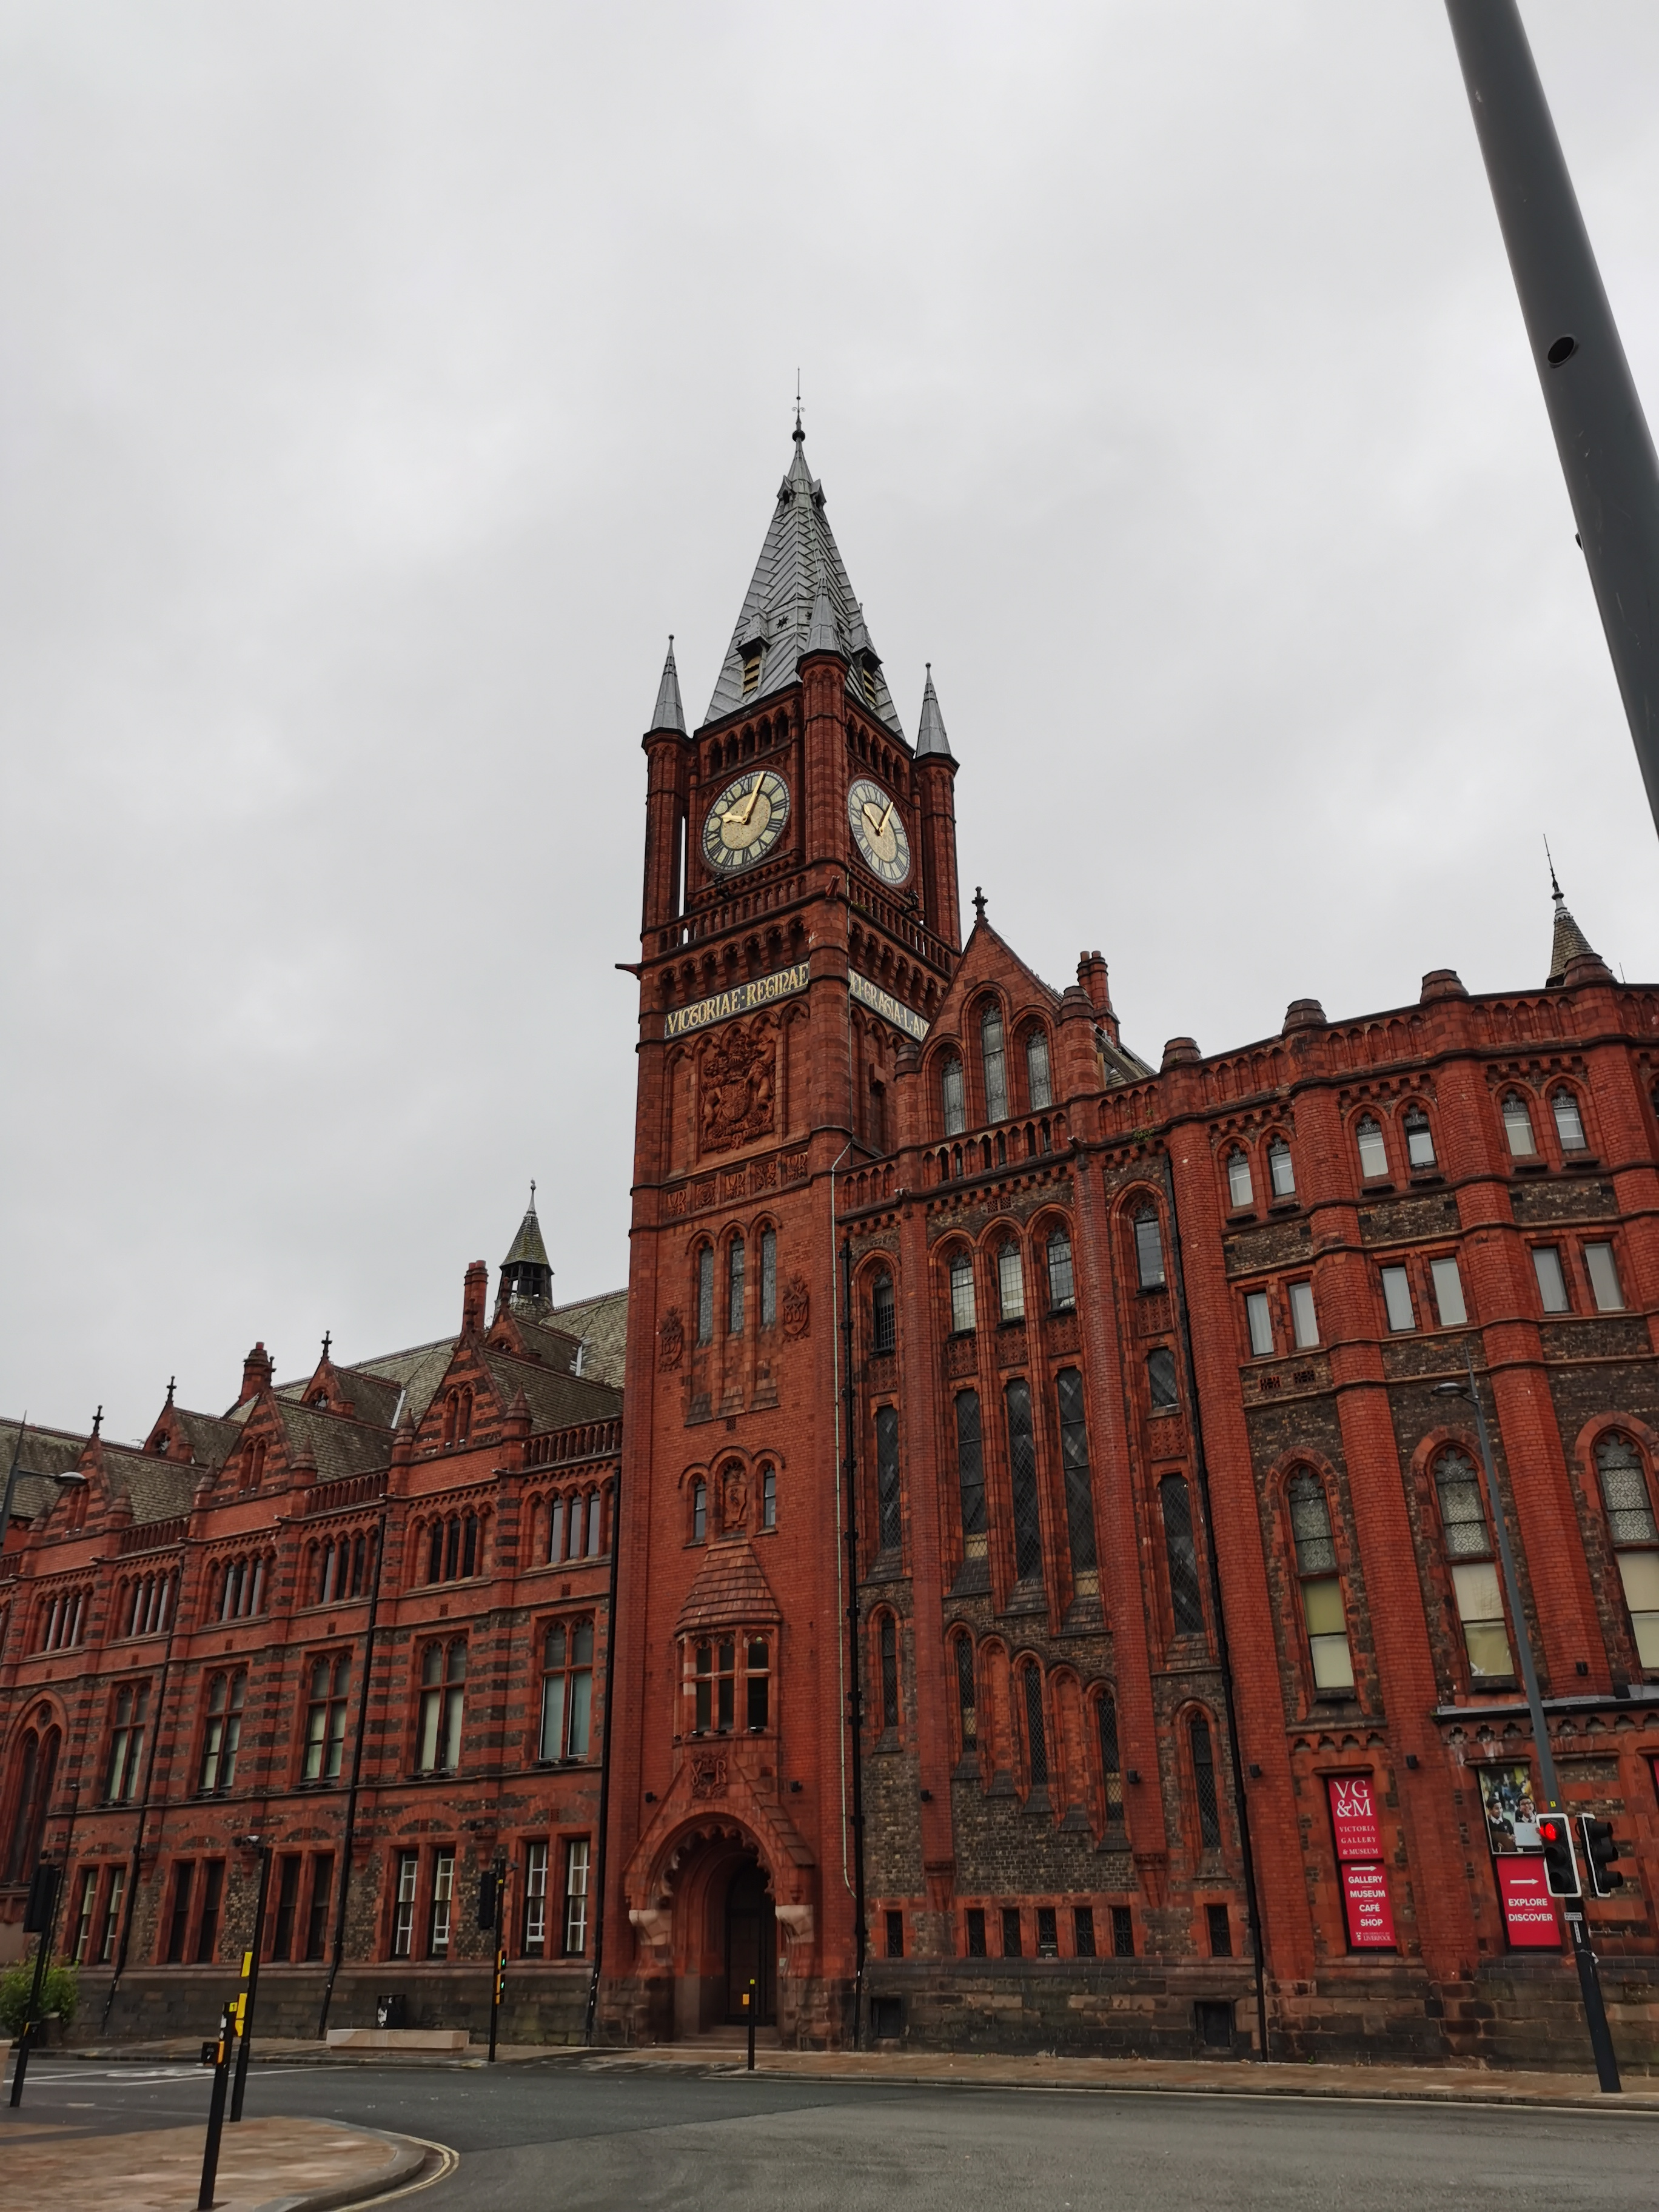
\includegraphics[width=\textwidth]{1E.jpg}
\end{figure}

\begin{figure}[H]
    \centering
    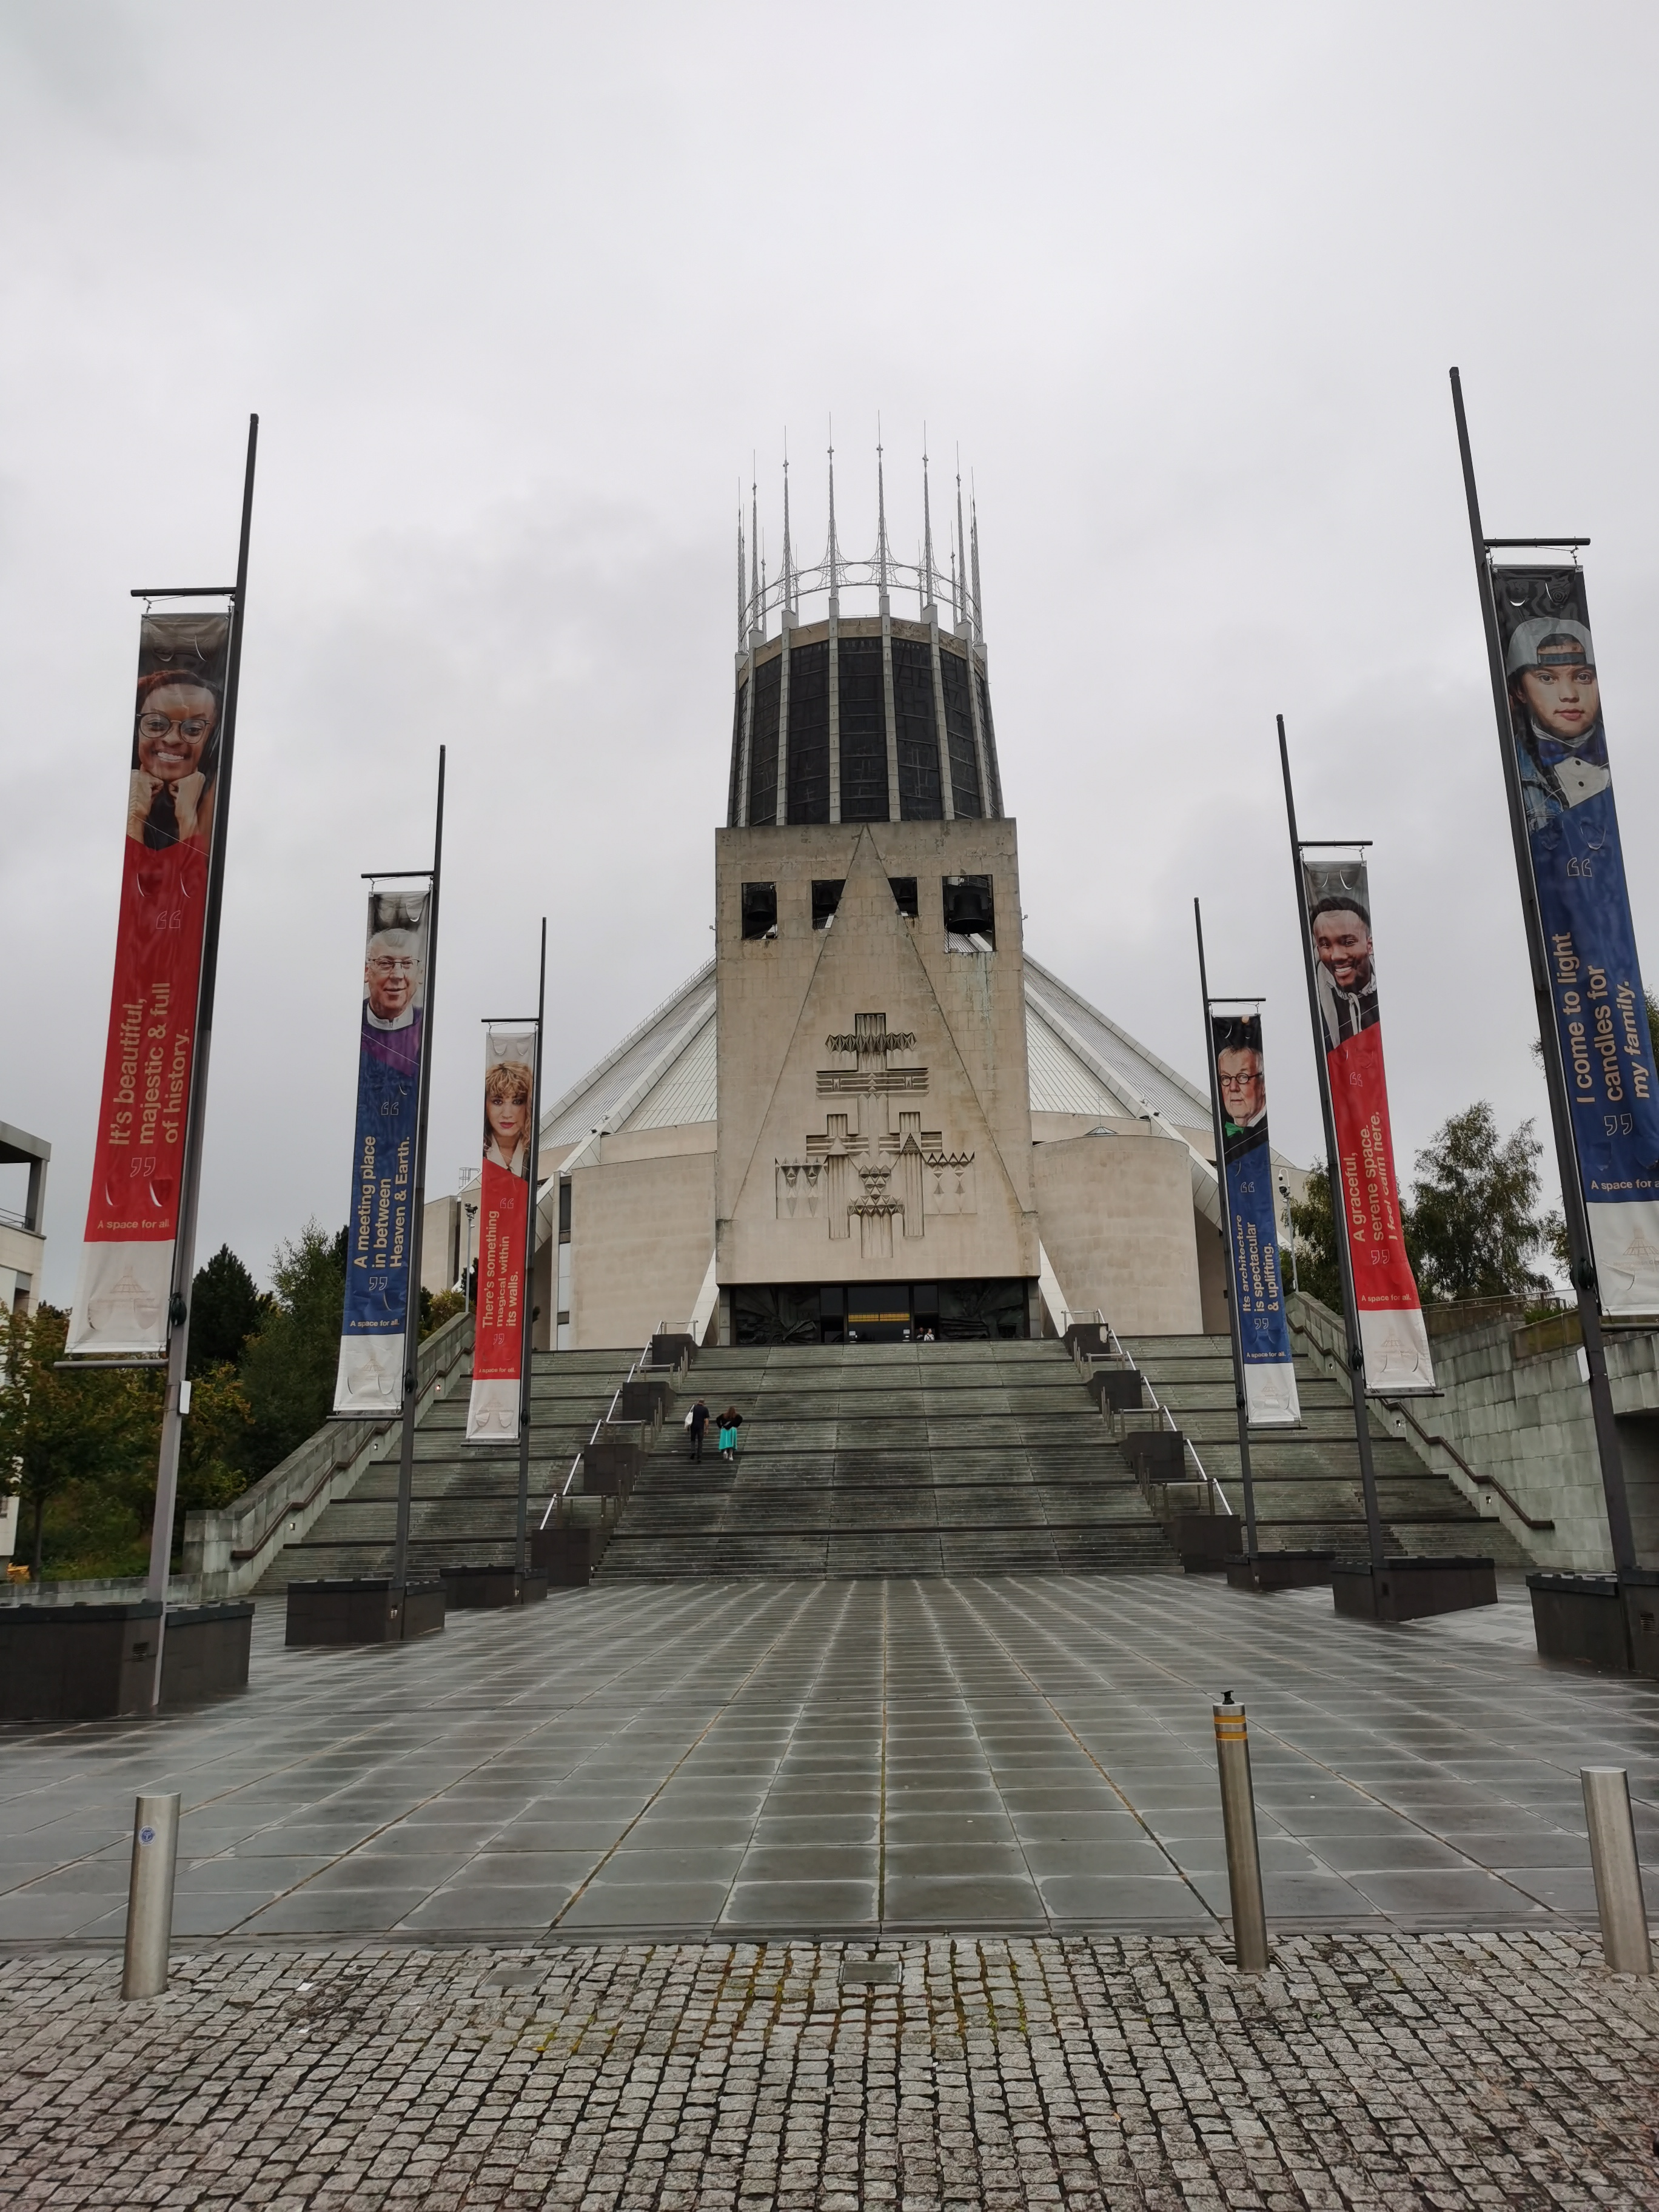
\includegraphics[width=\textwidth]{1F.jpg}
\end{figure}

\begin{figure}[H]
    \centering
    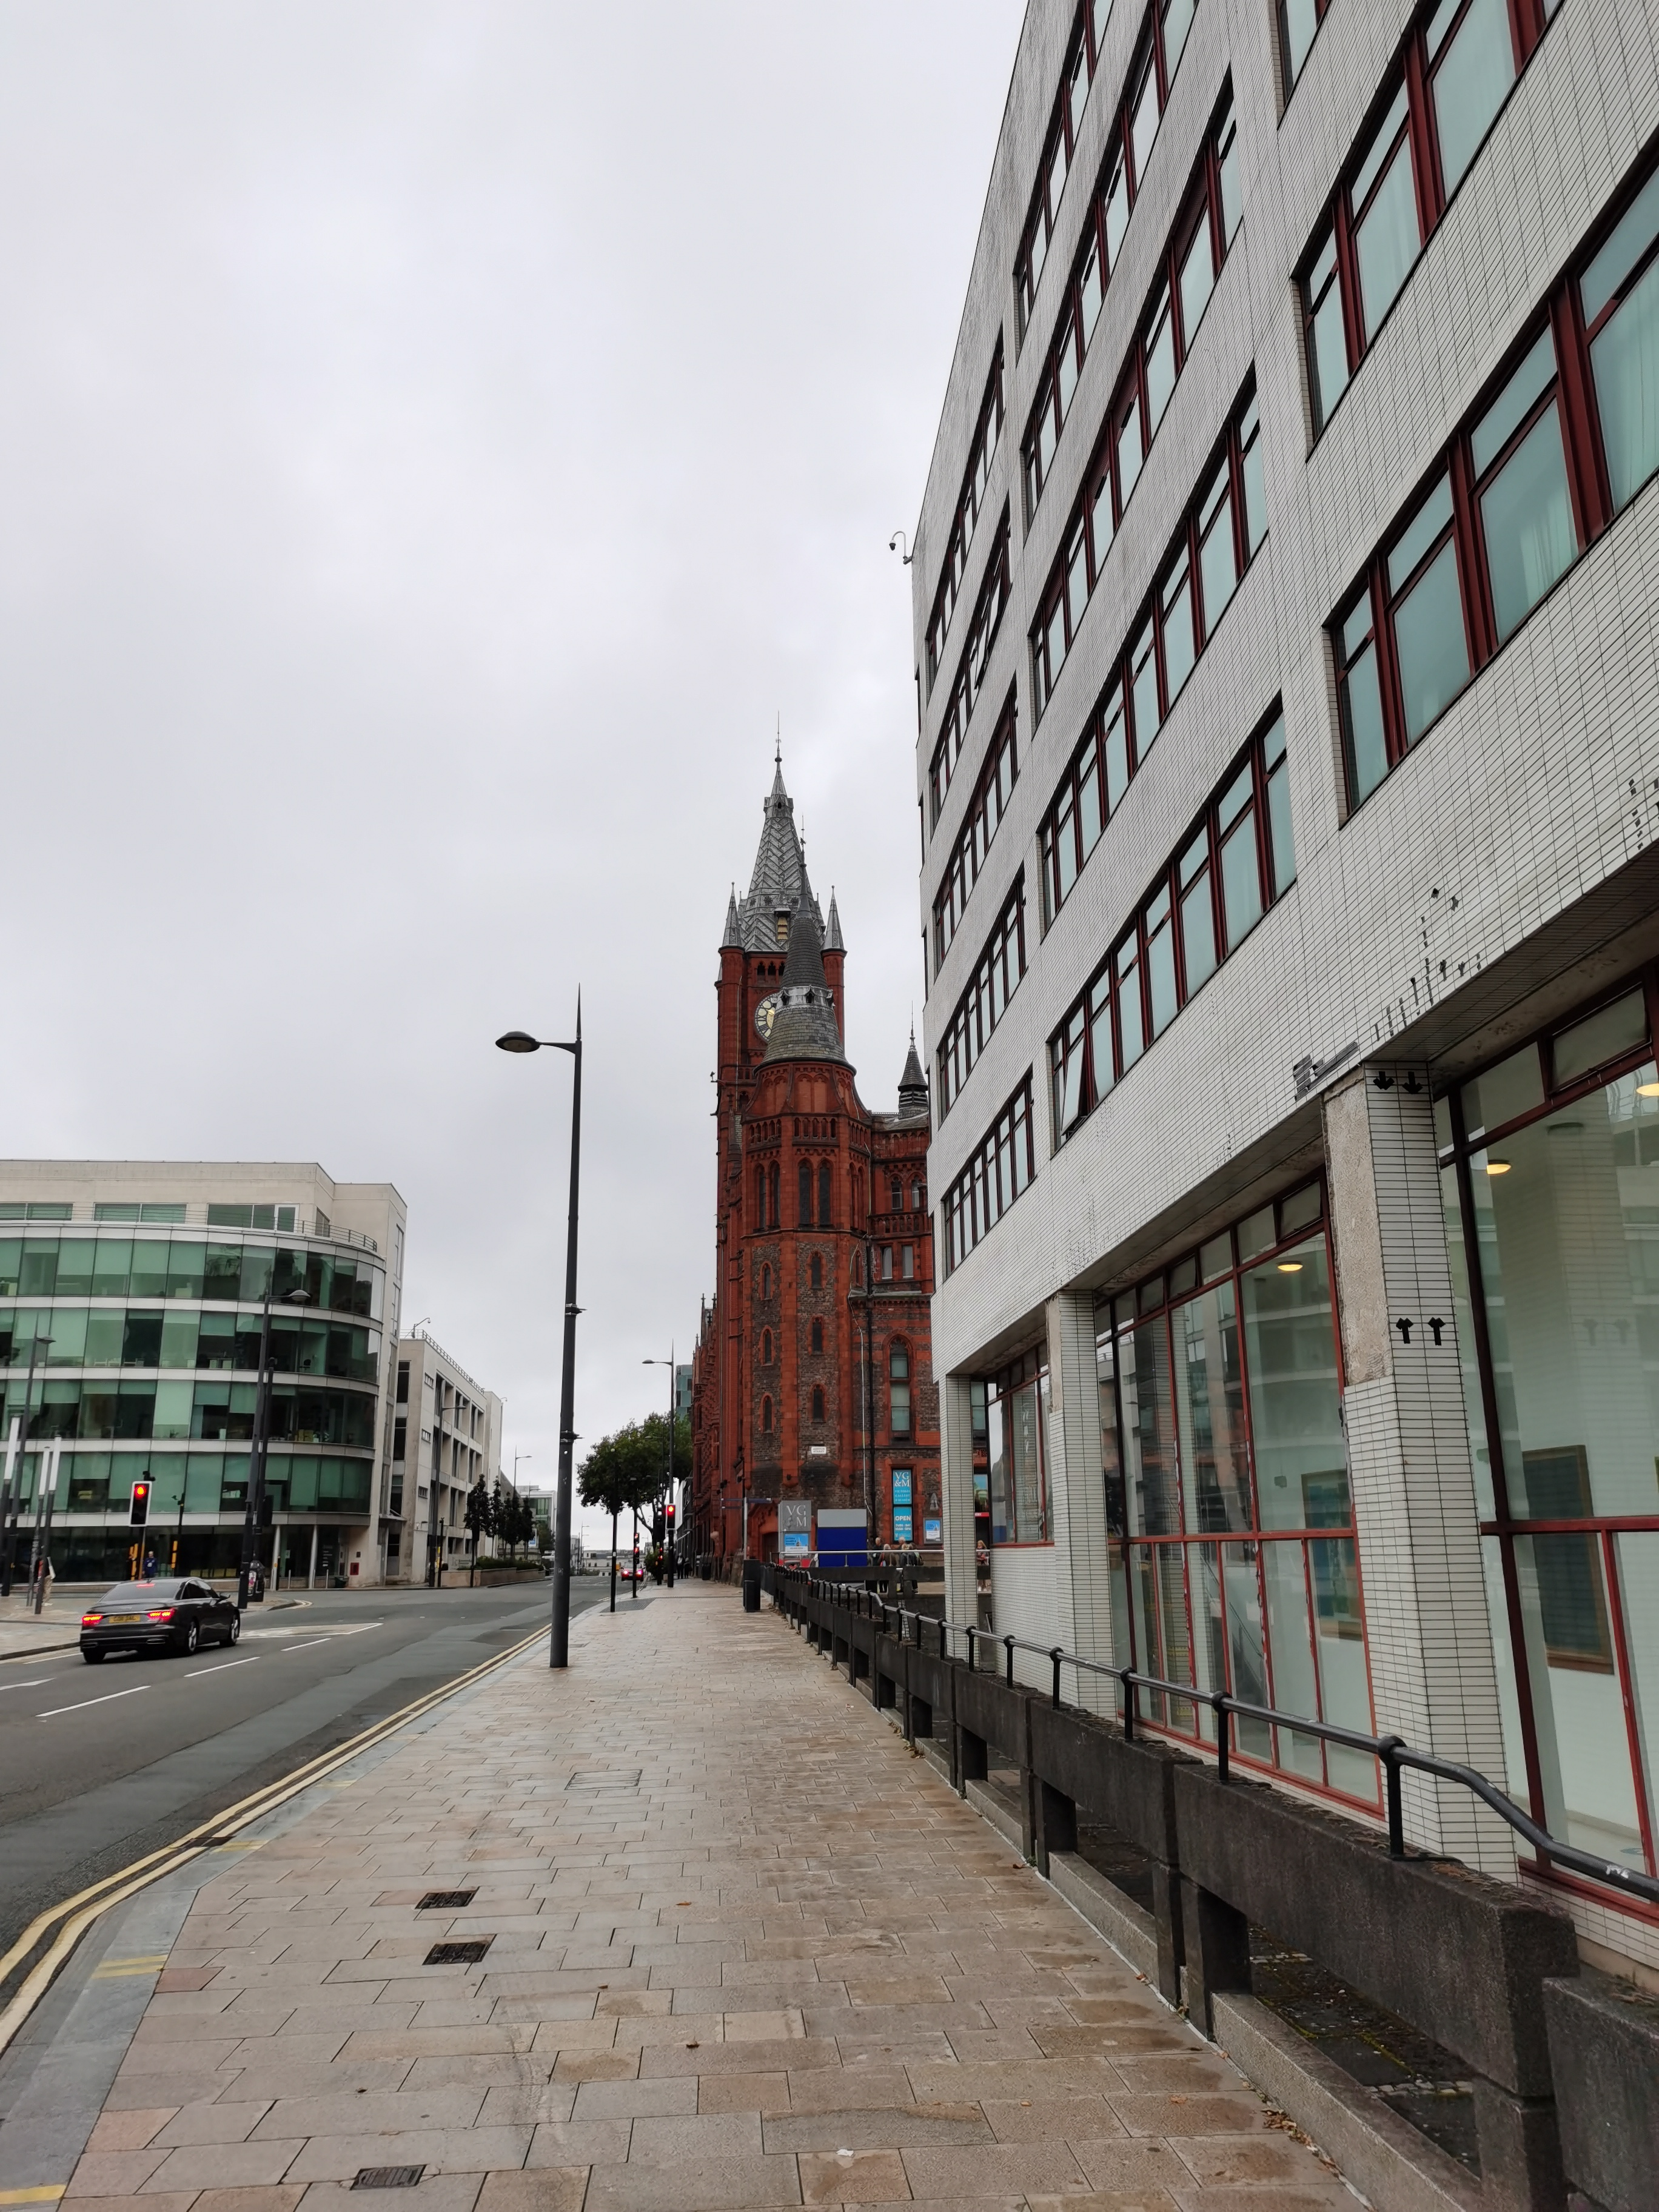
\includegraphics[width=\textwidth]{1G.jpg}
\end{figure}

\begin{figure}[H]
    \centering
    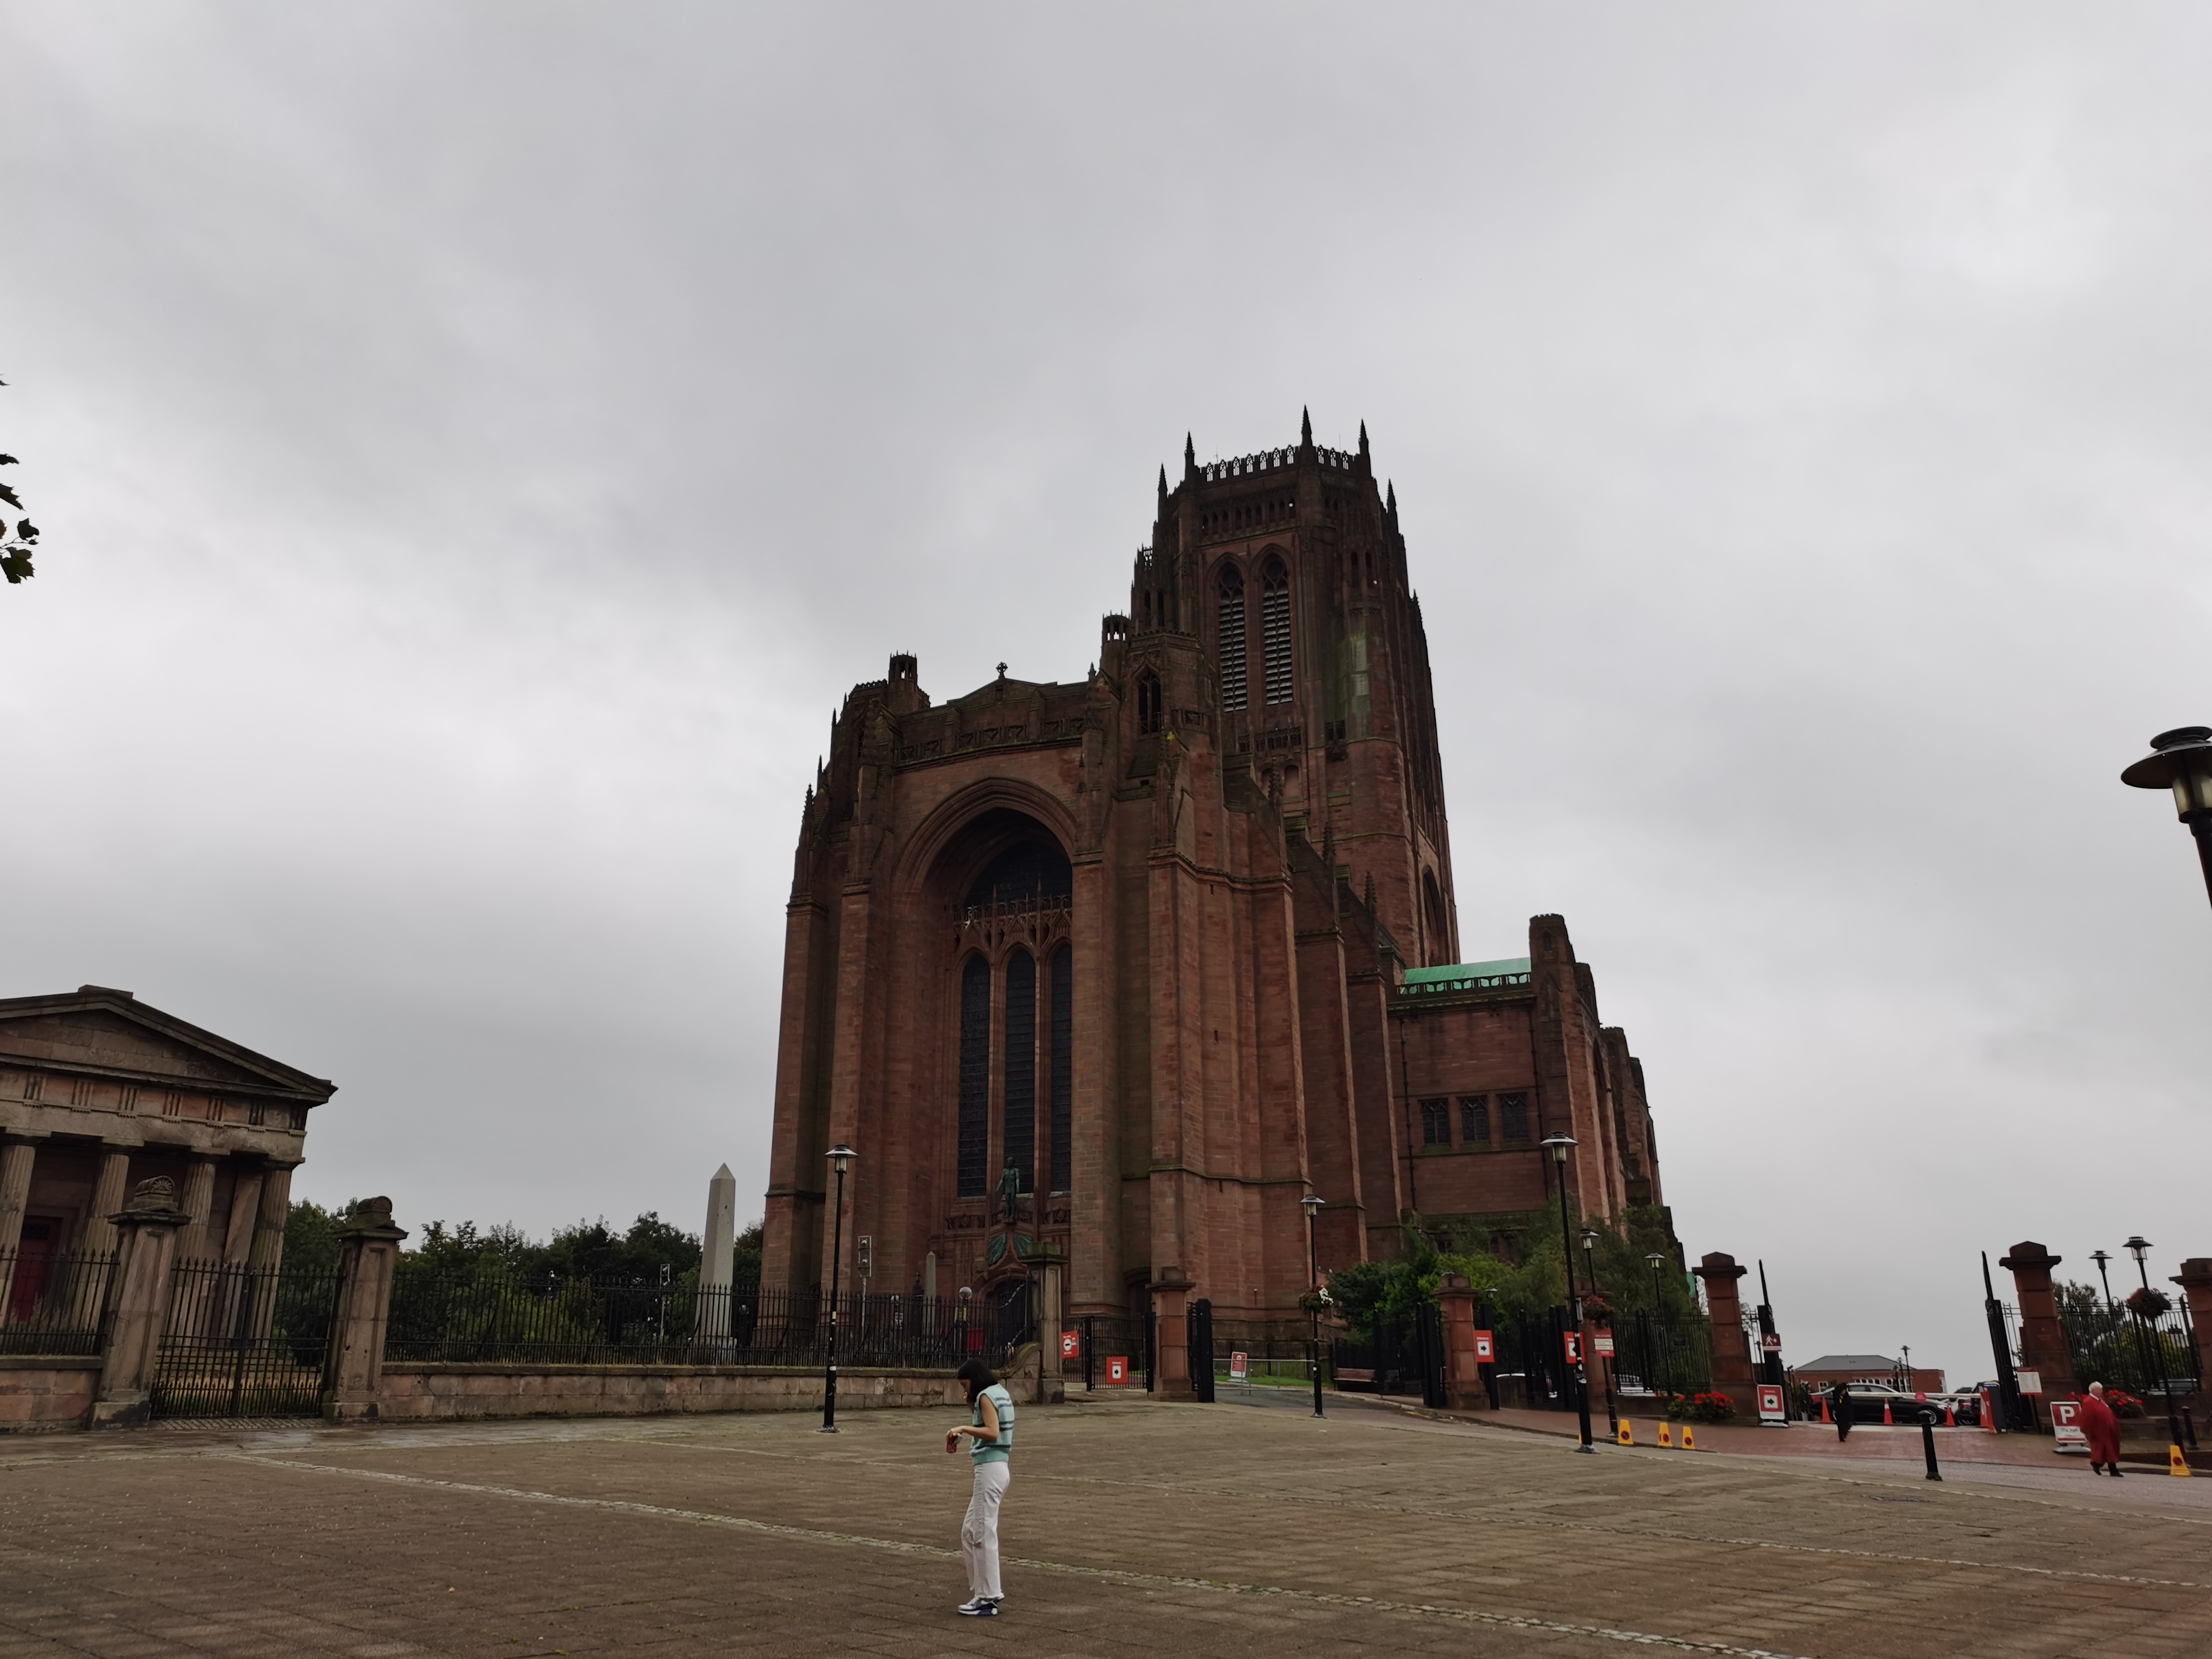
\includegraphics[width=\textwidth]{1H.jpg}
\end{figure}

\begin{figure}[H]
    \centering
    \includegraphics[width=\textwidth]{1I.jpg}
\end{figure}

\begin{figure}[H]
    \centering
    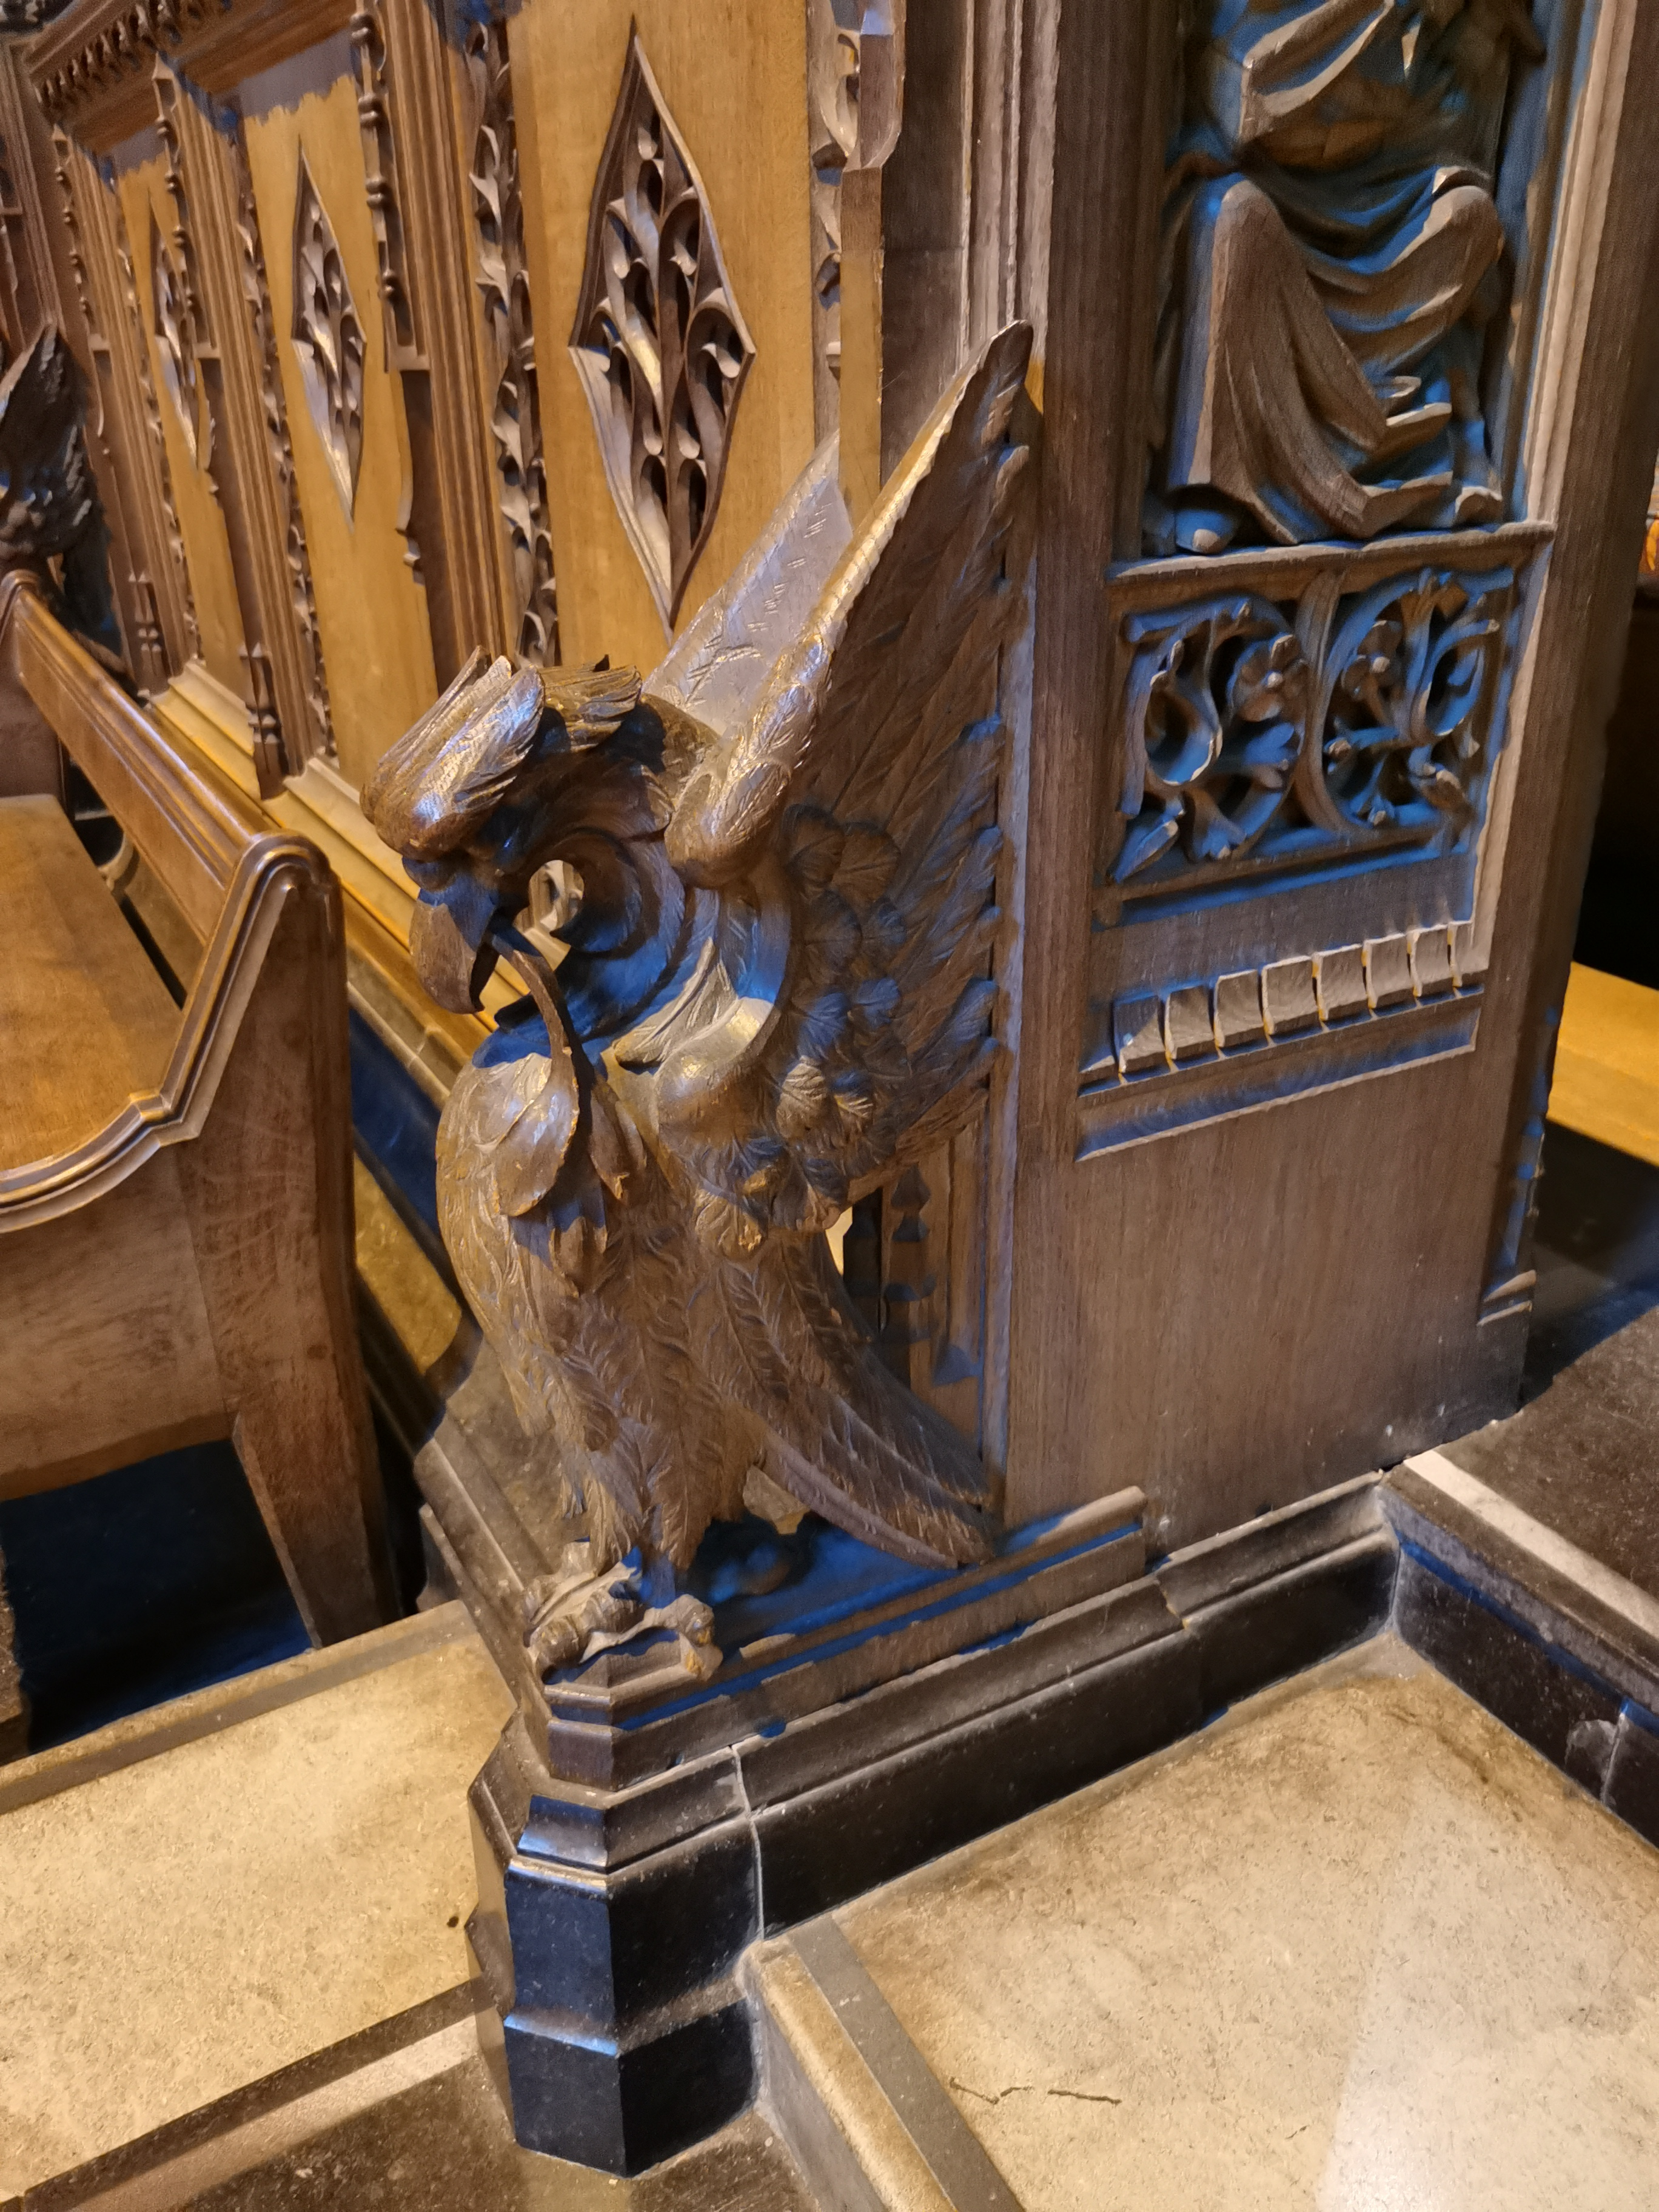
\includegraphics[width=\textwidth]{1J.jpg}
\end{figure}

\begin{figure}[H]
    \centering
    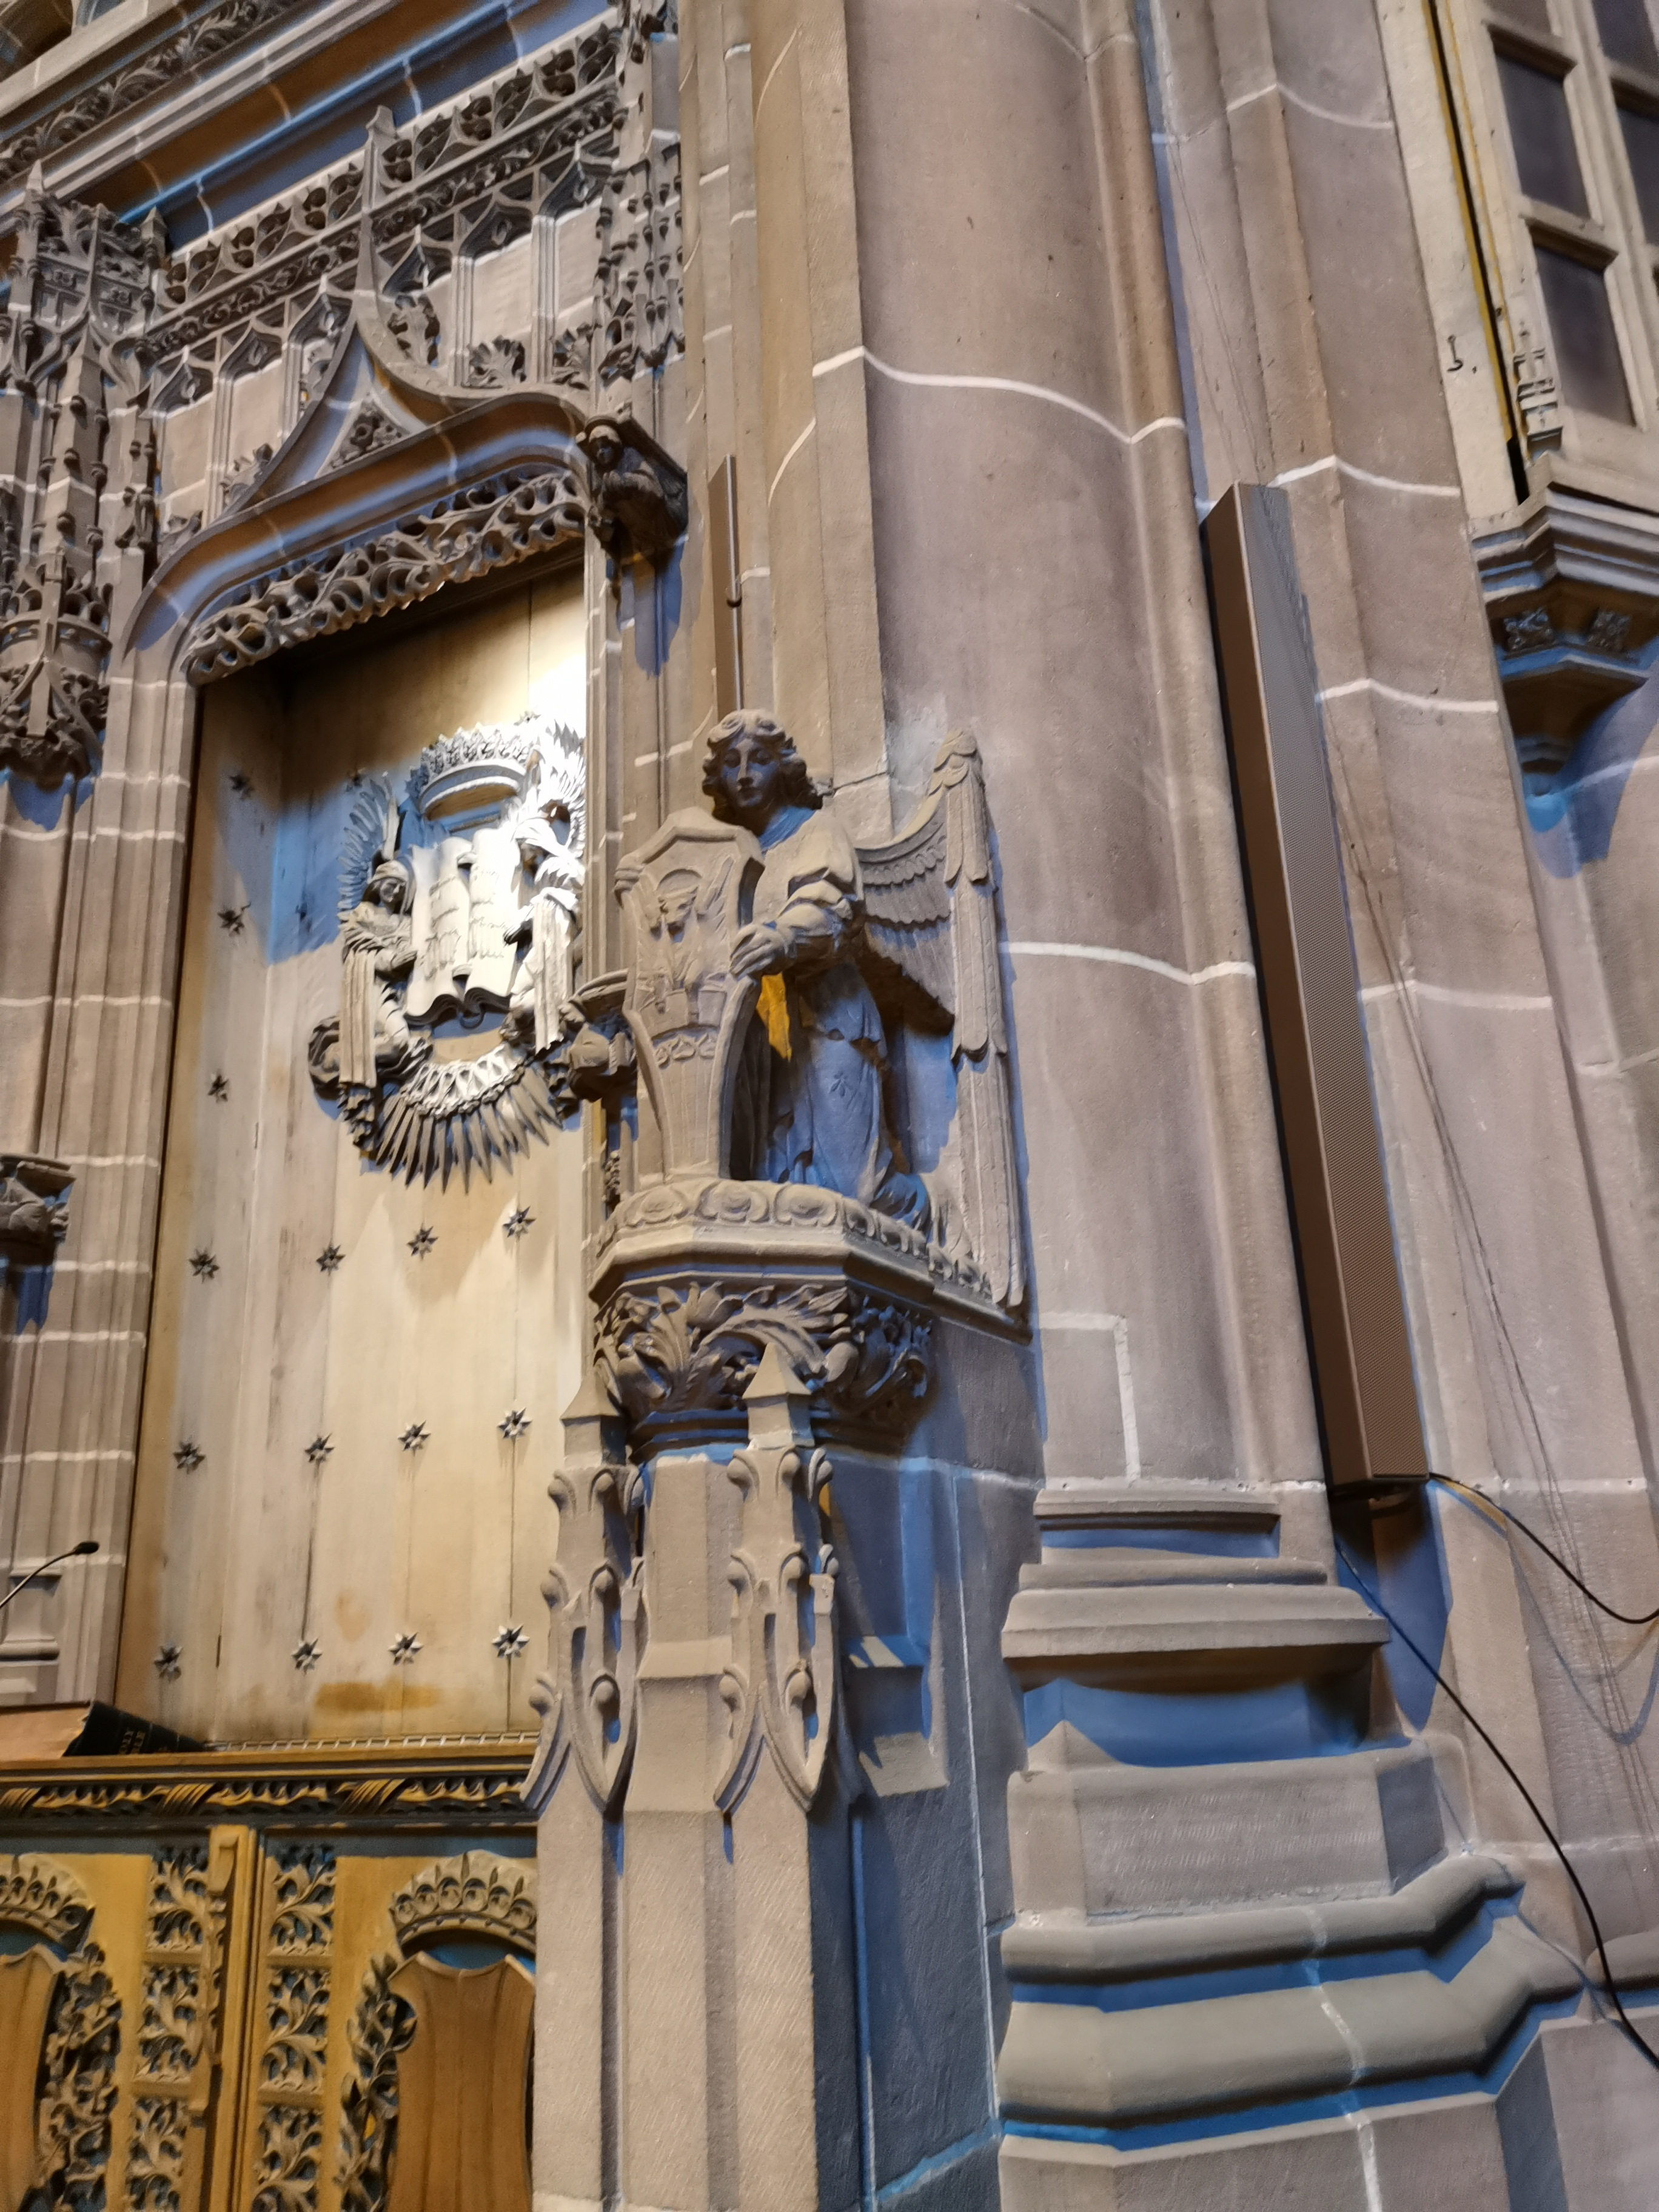
\includegraphics[width=\textwidth]{1K.jpg}
\end{figure}

\begin{figure}[H]
    \centering
    \includegraphics[width=\textwidth]{1L.jpg}
\end{figure}

\begin{figure}[H]
    \centering
    \includegraphics[width=\textwidth]{1M.jpg}
\end{figure}

\begin{figure}[H]
    \centering
    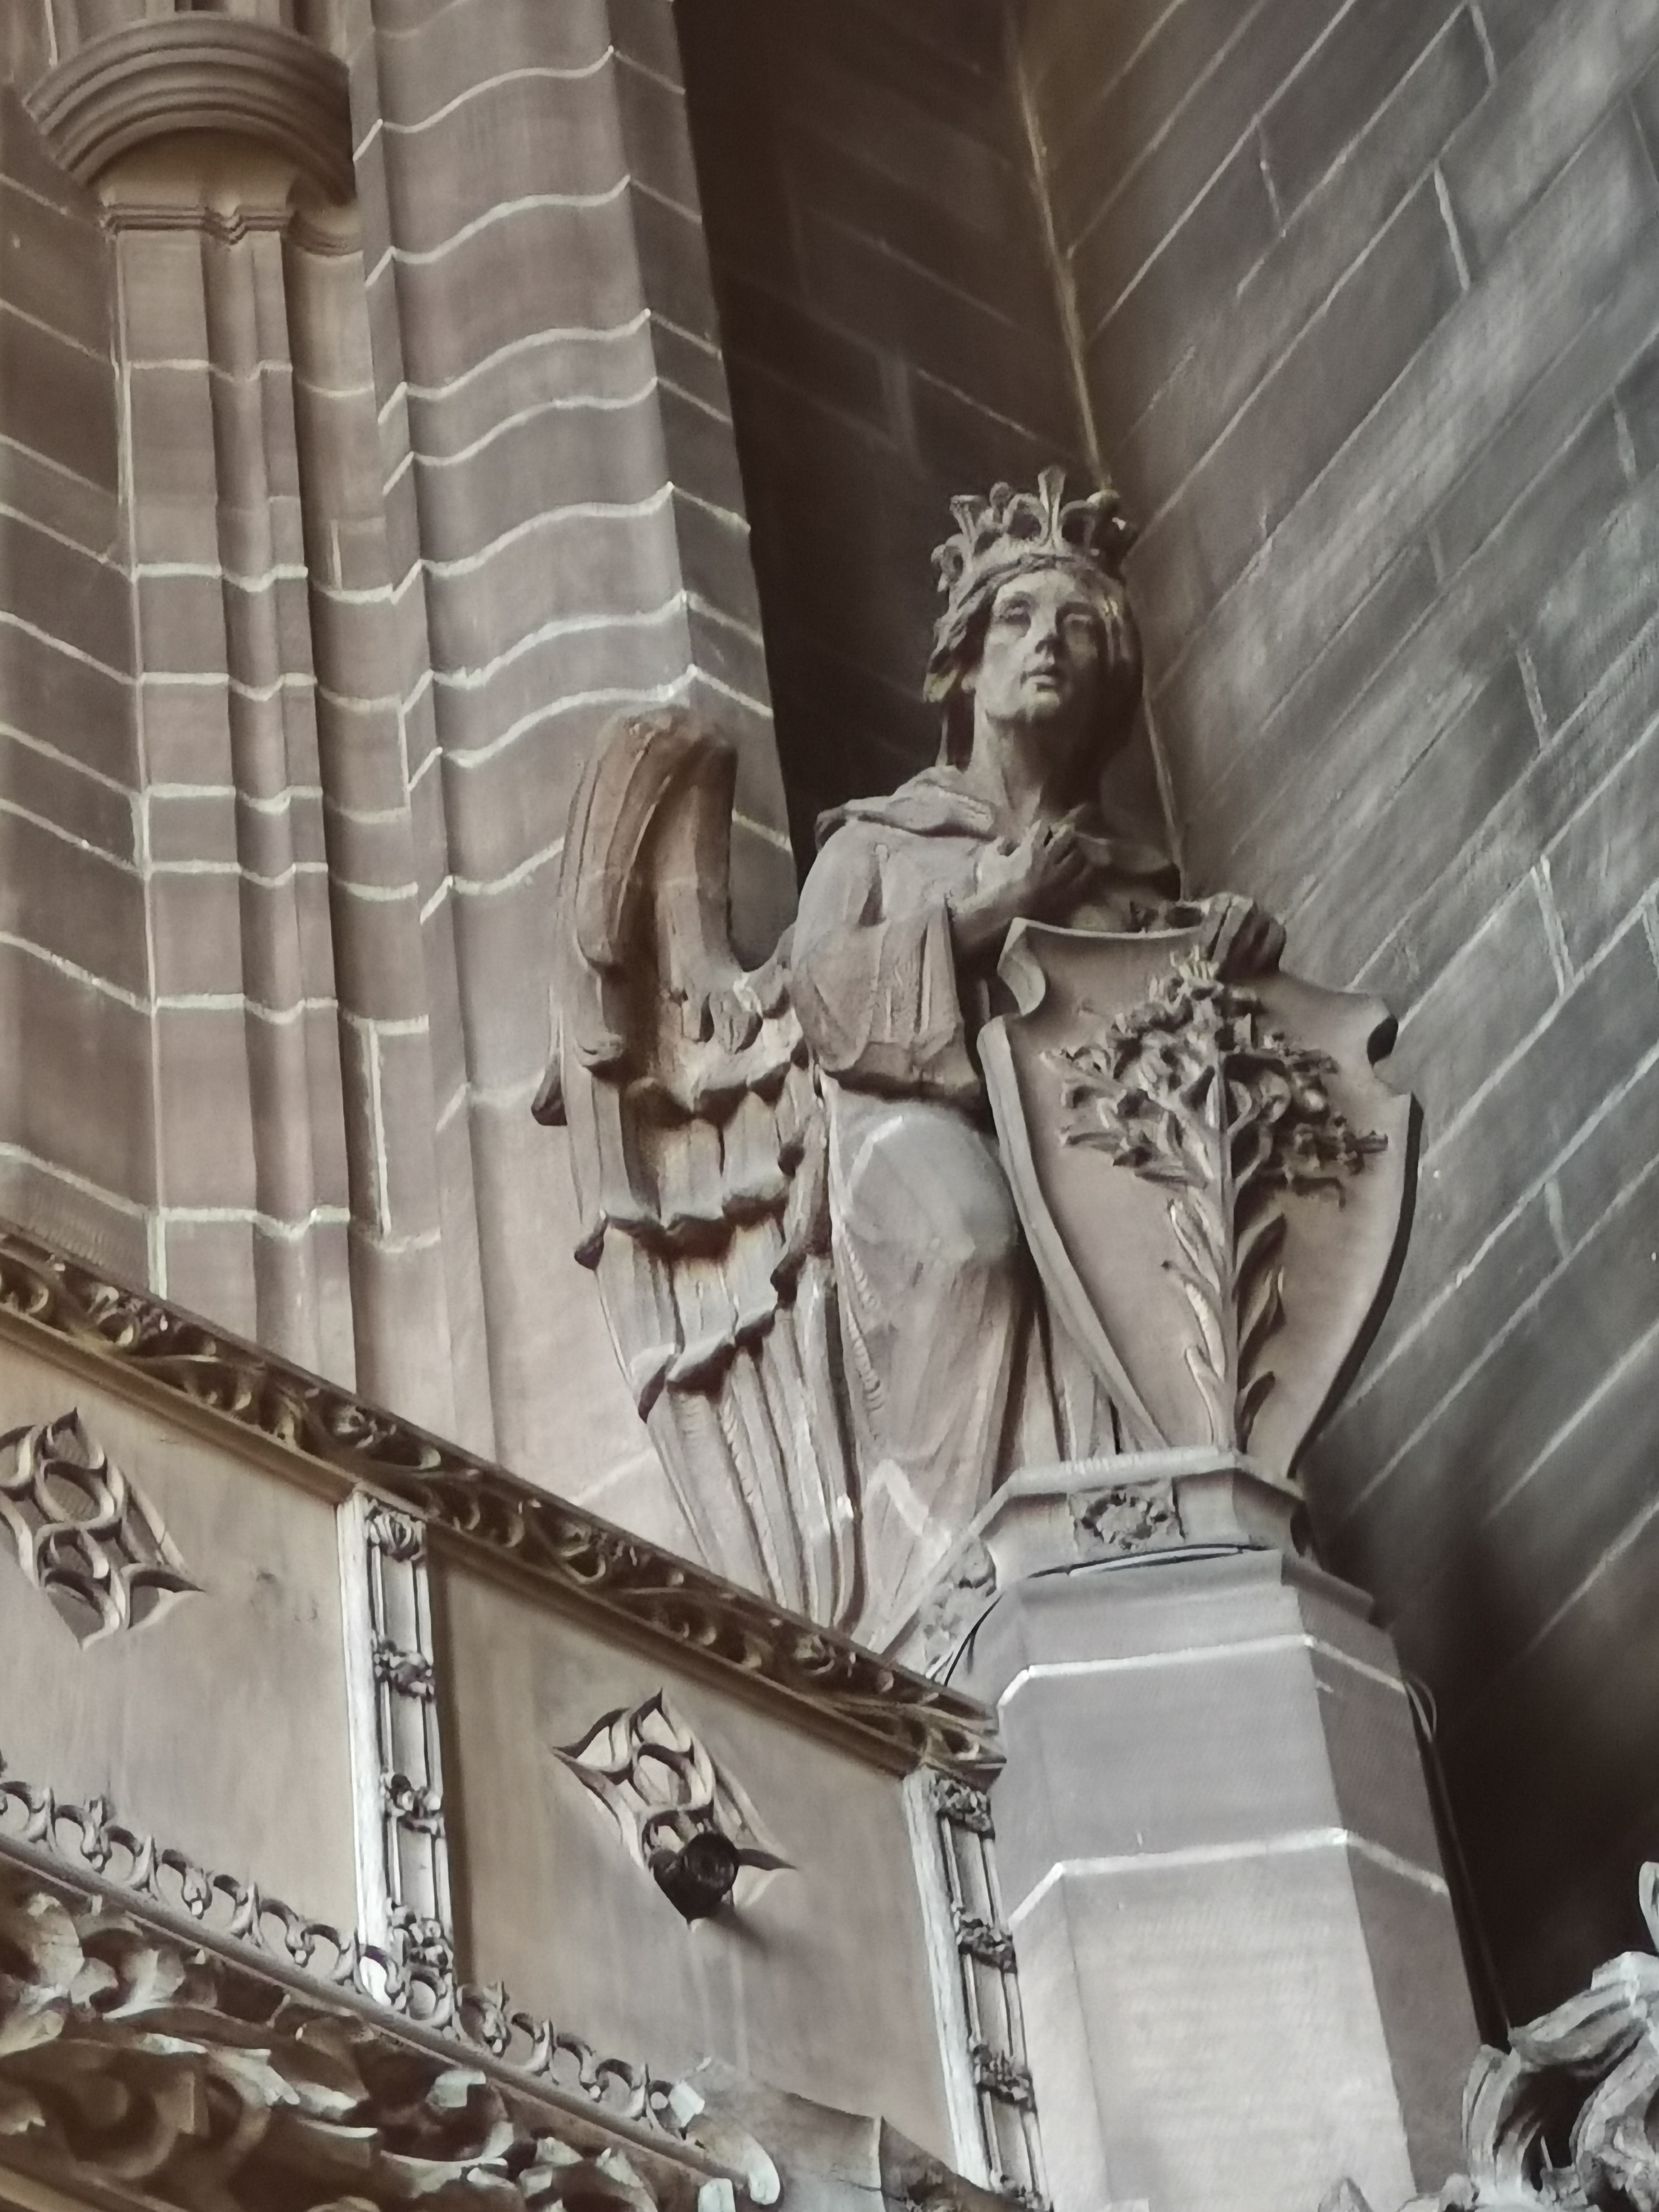
\includegraphics[width=\textwidth]{1N.jpg}
\end{figure}

\begin{figure}[H]
    \centering
    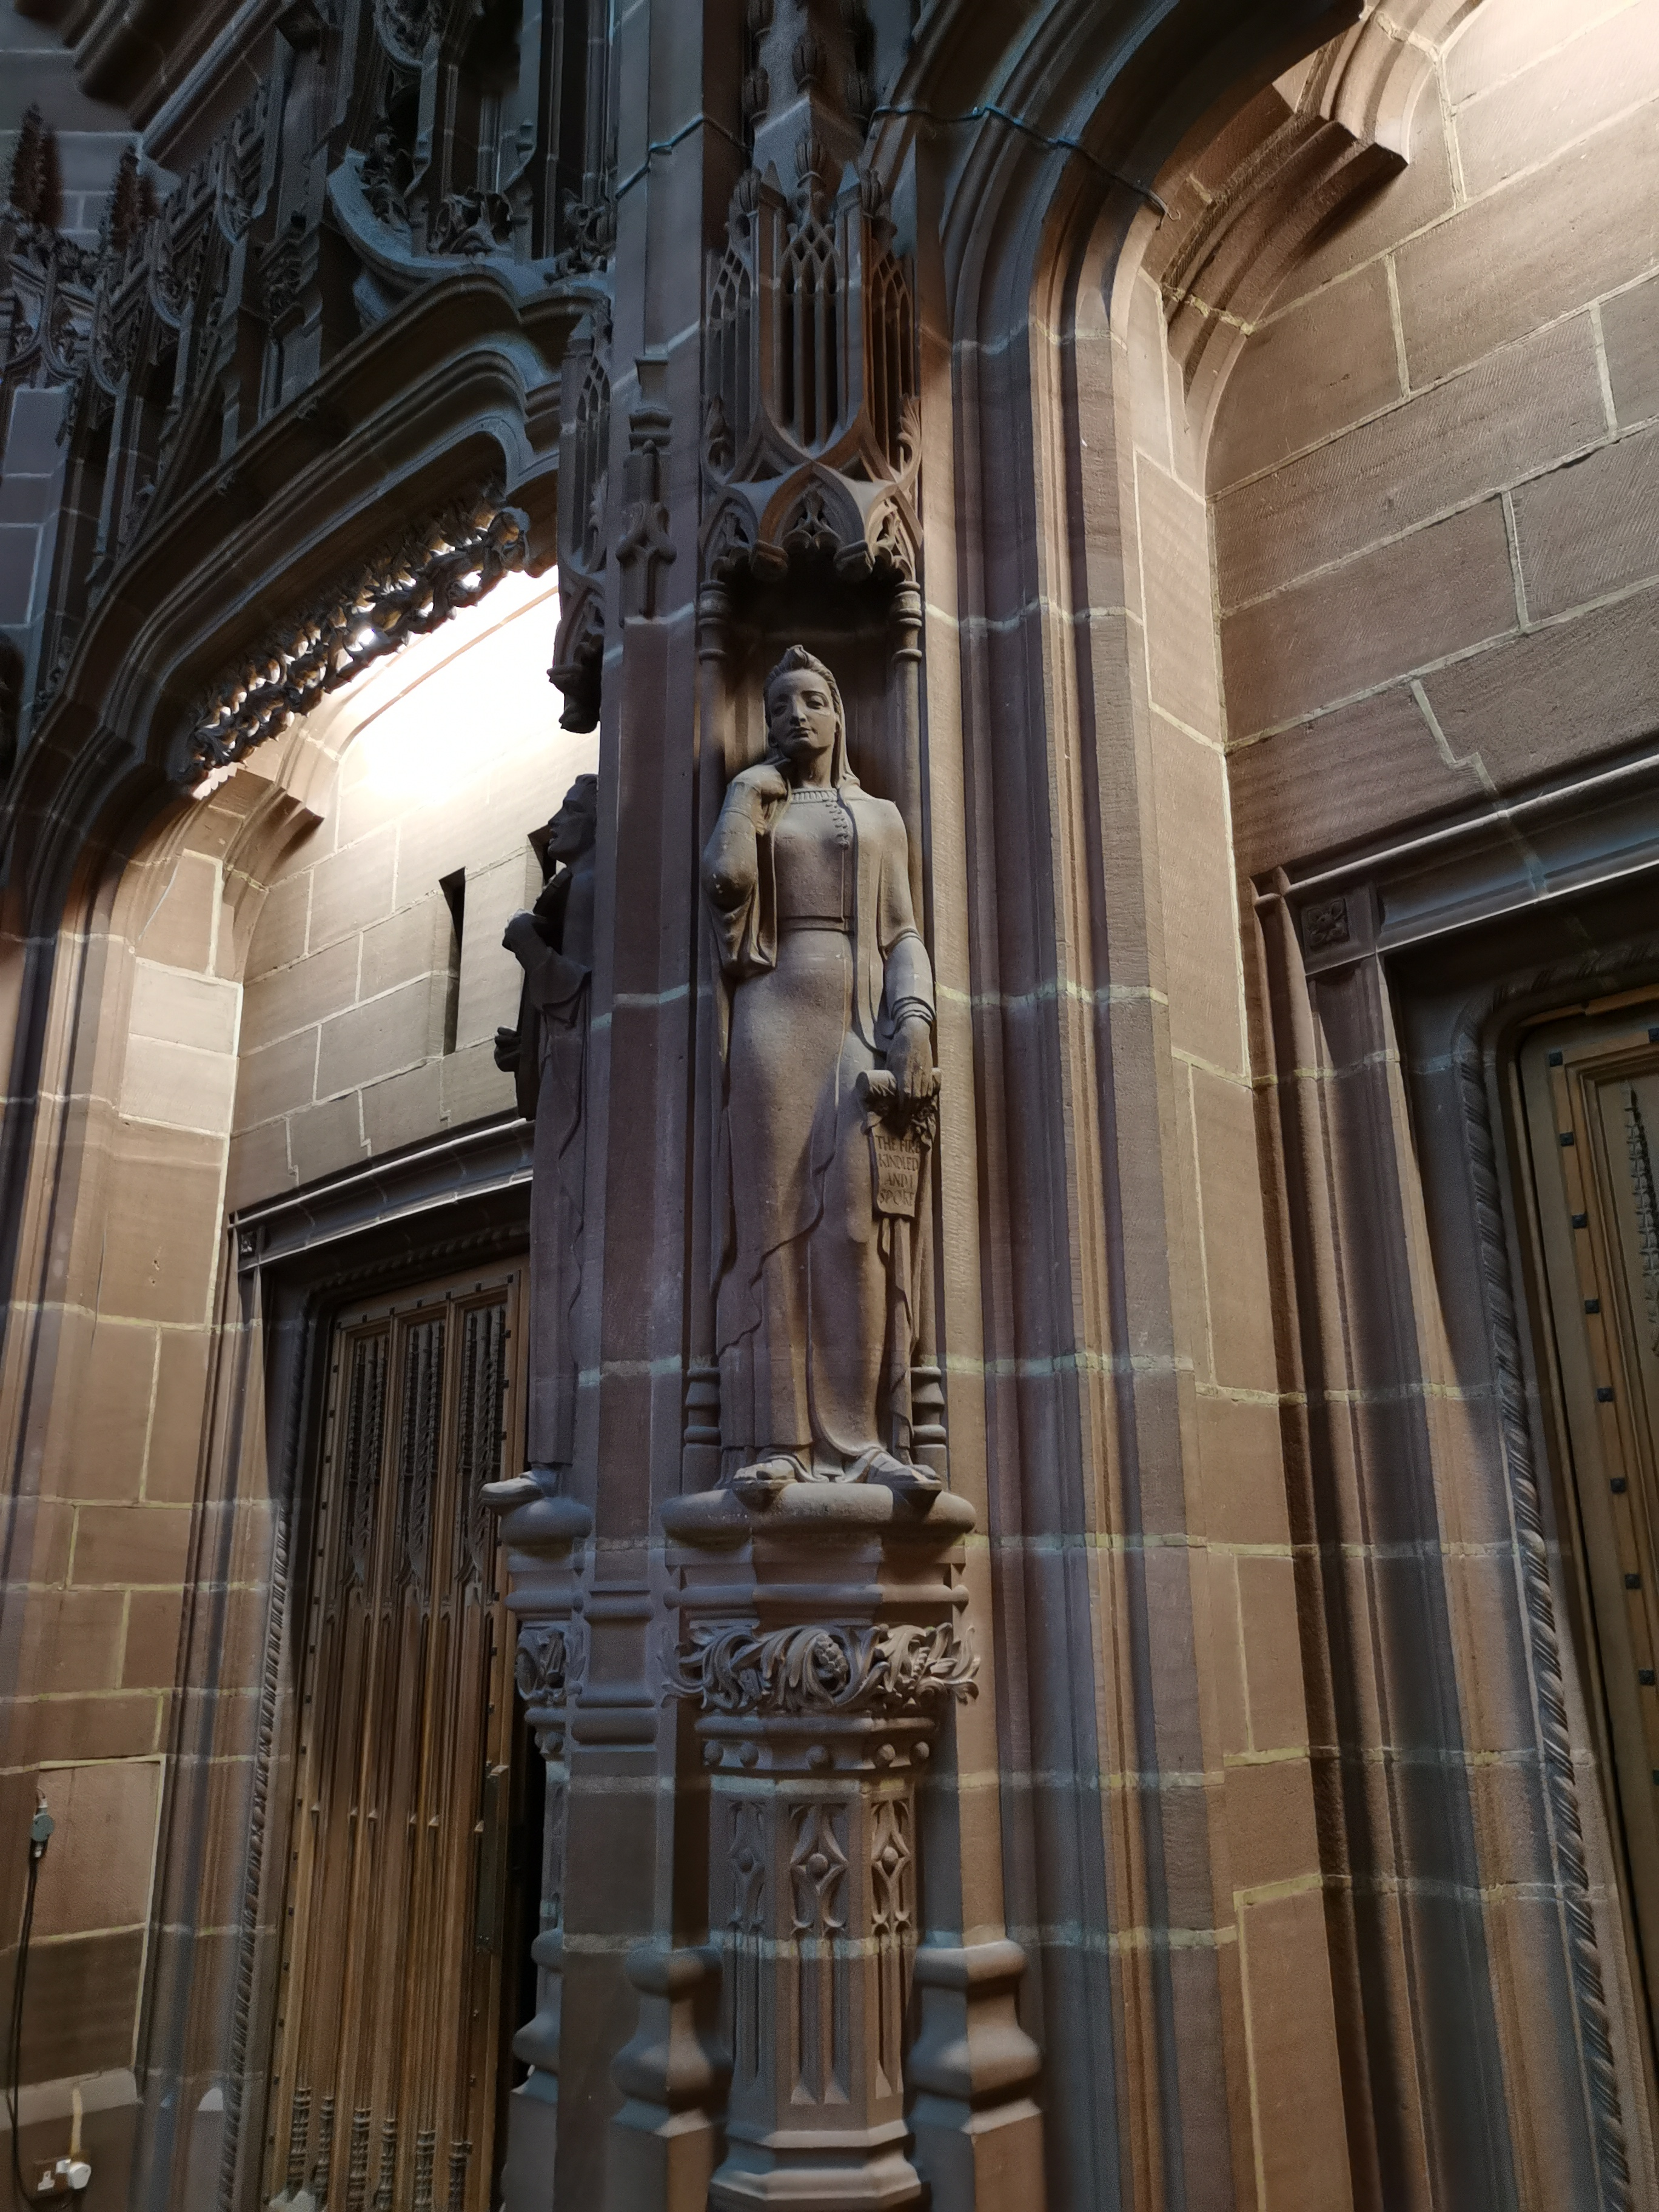
\includegraphics[width=\textwidth]{1O.jpg}
\end{figure}

\begin{figure}[H]
    \centering
    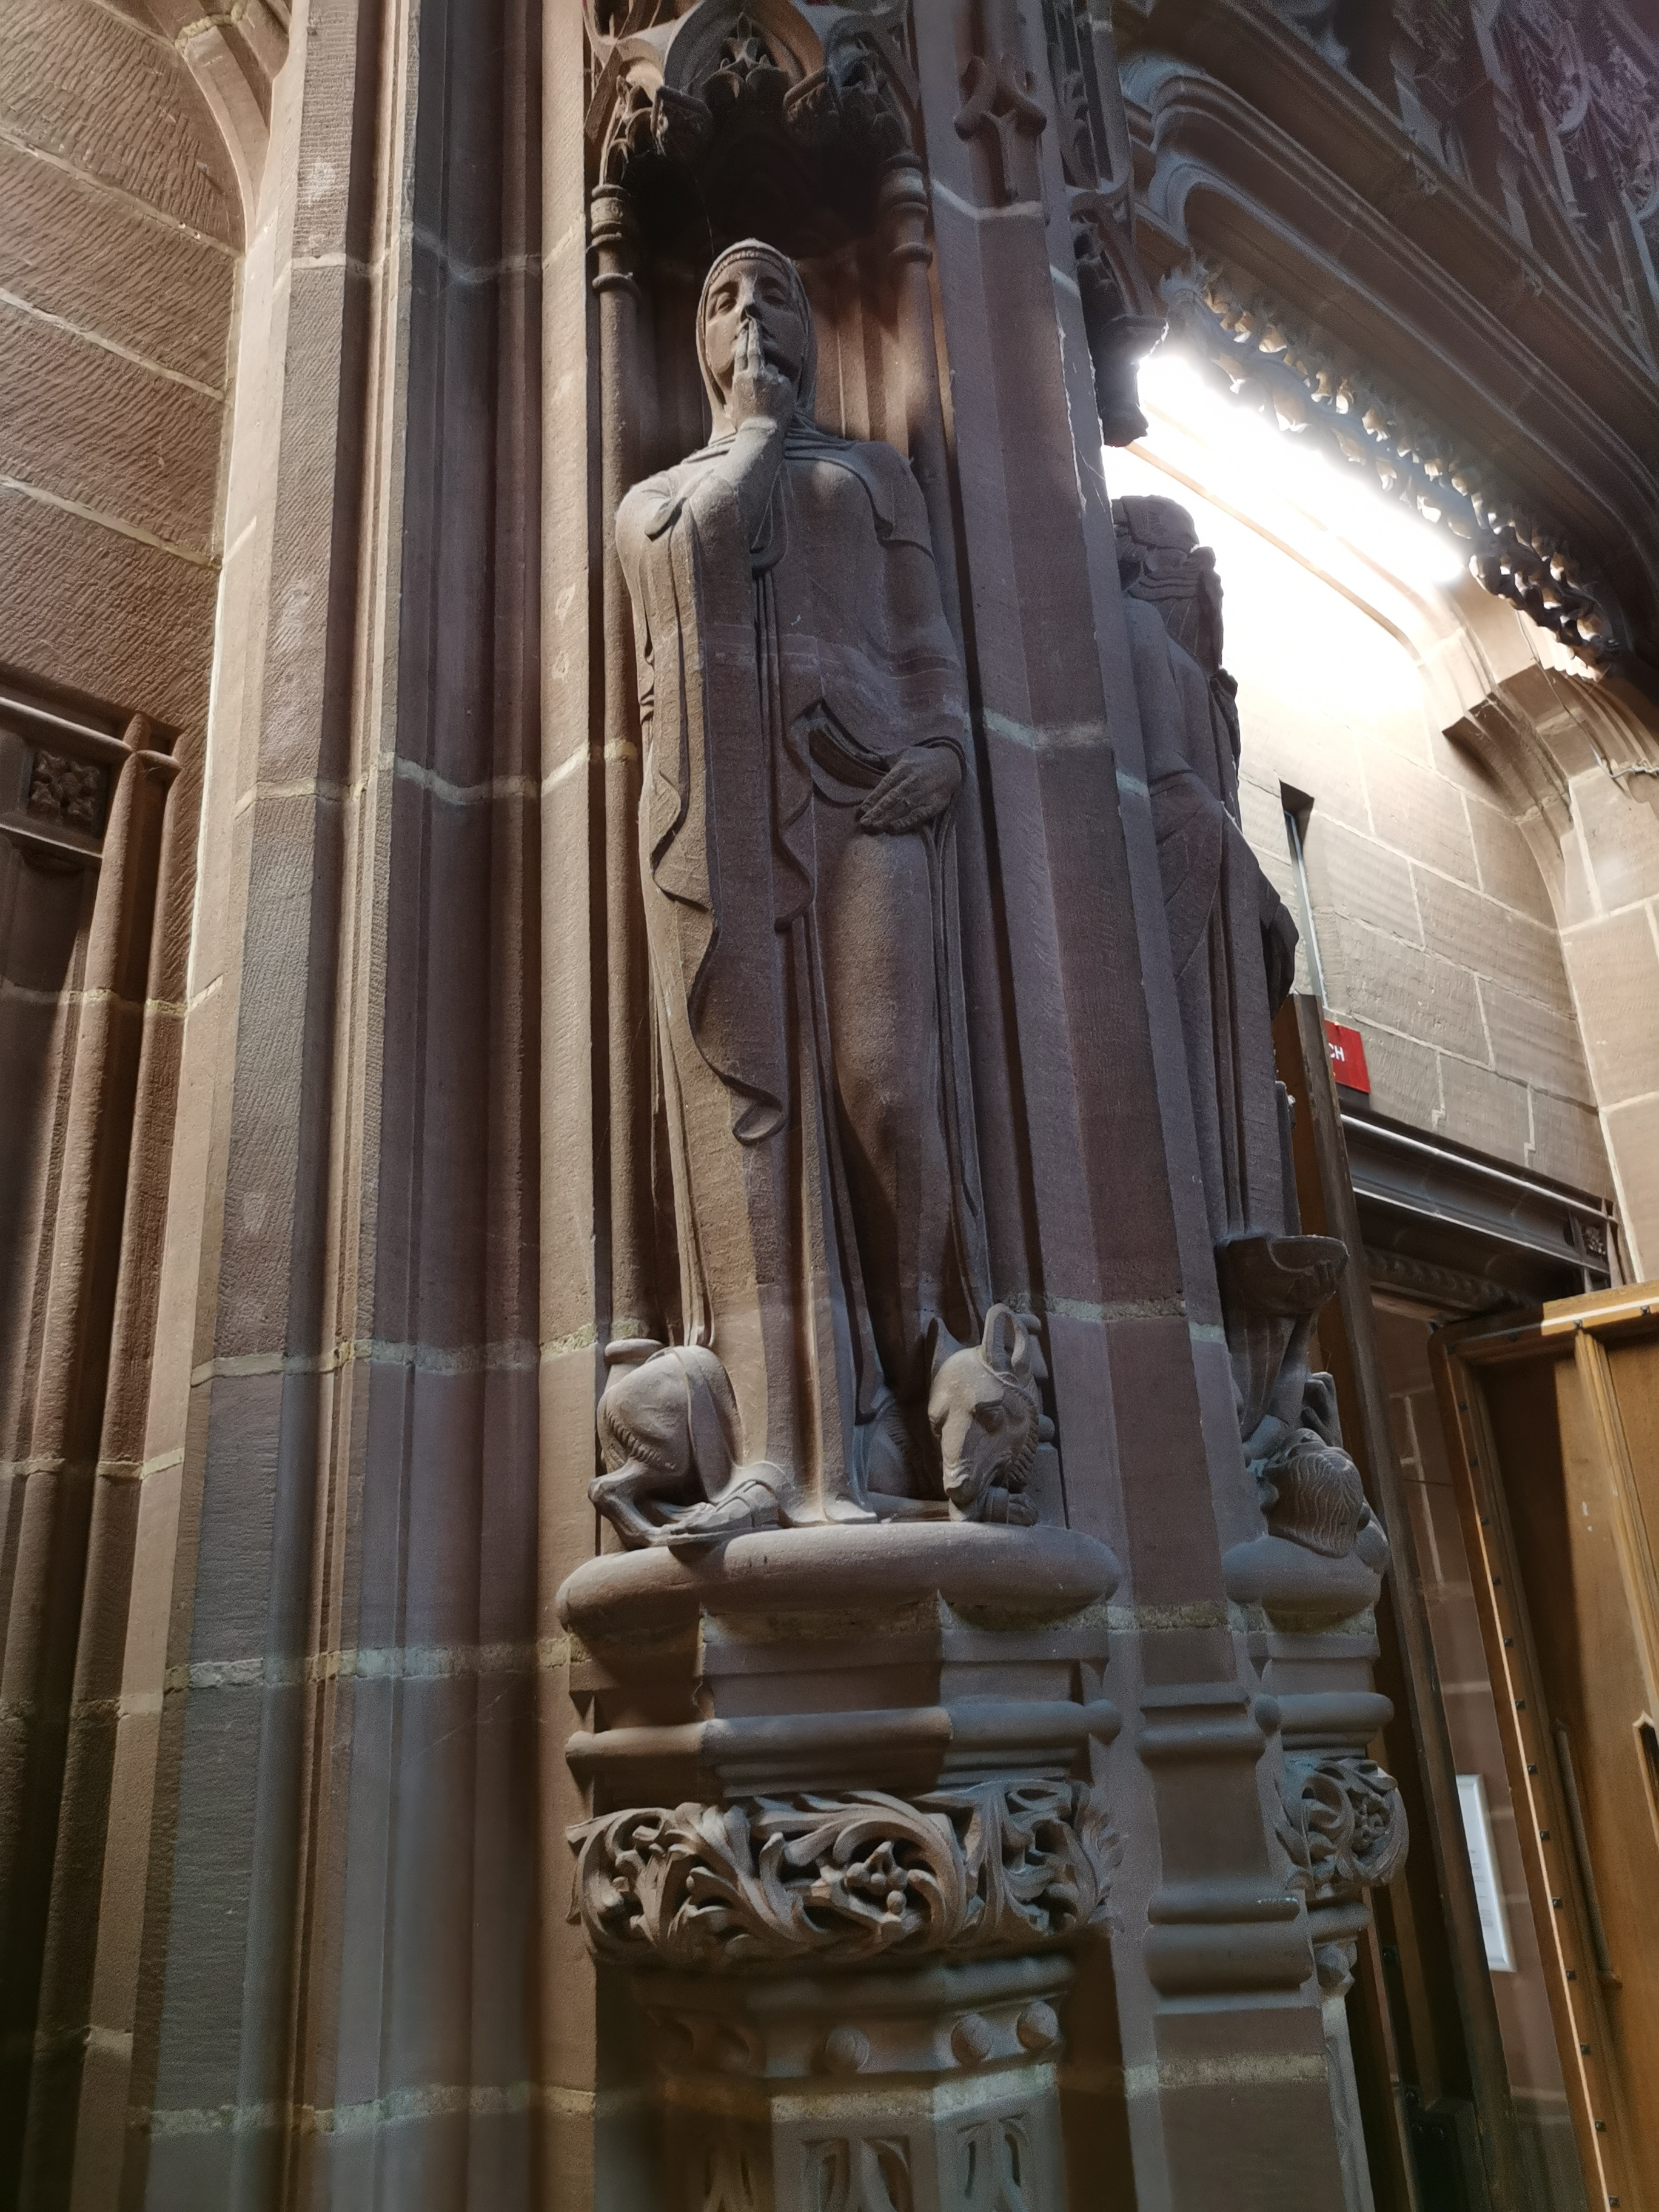
\includegraphics[width=\textwidth]{1P.jpg}
\end{figure}
  
\begin{figure}[H]
    \centering
    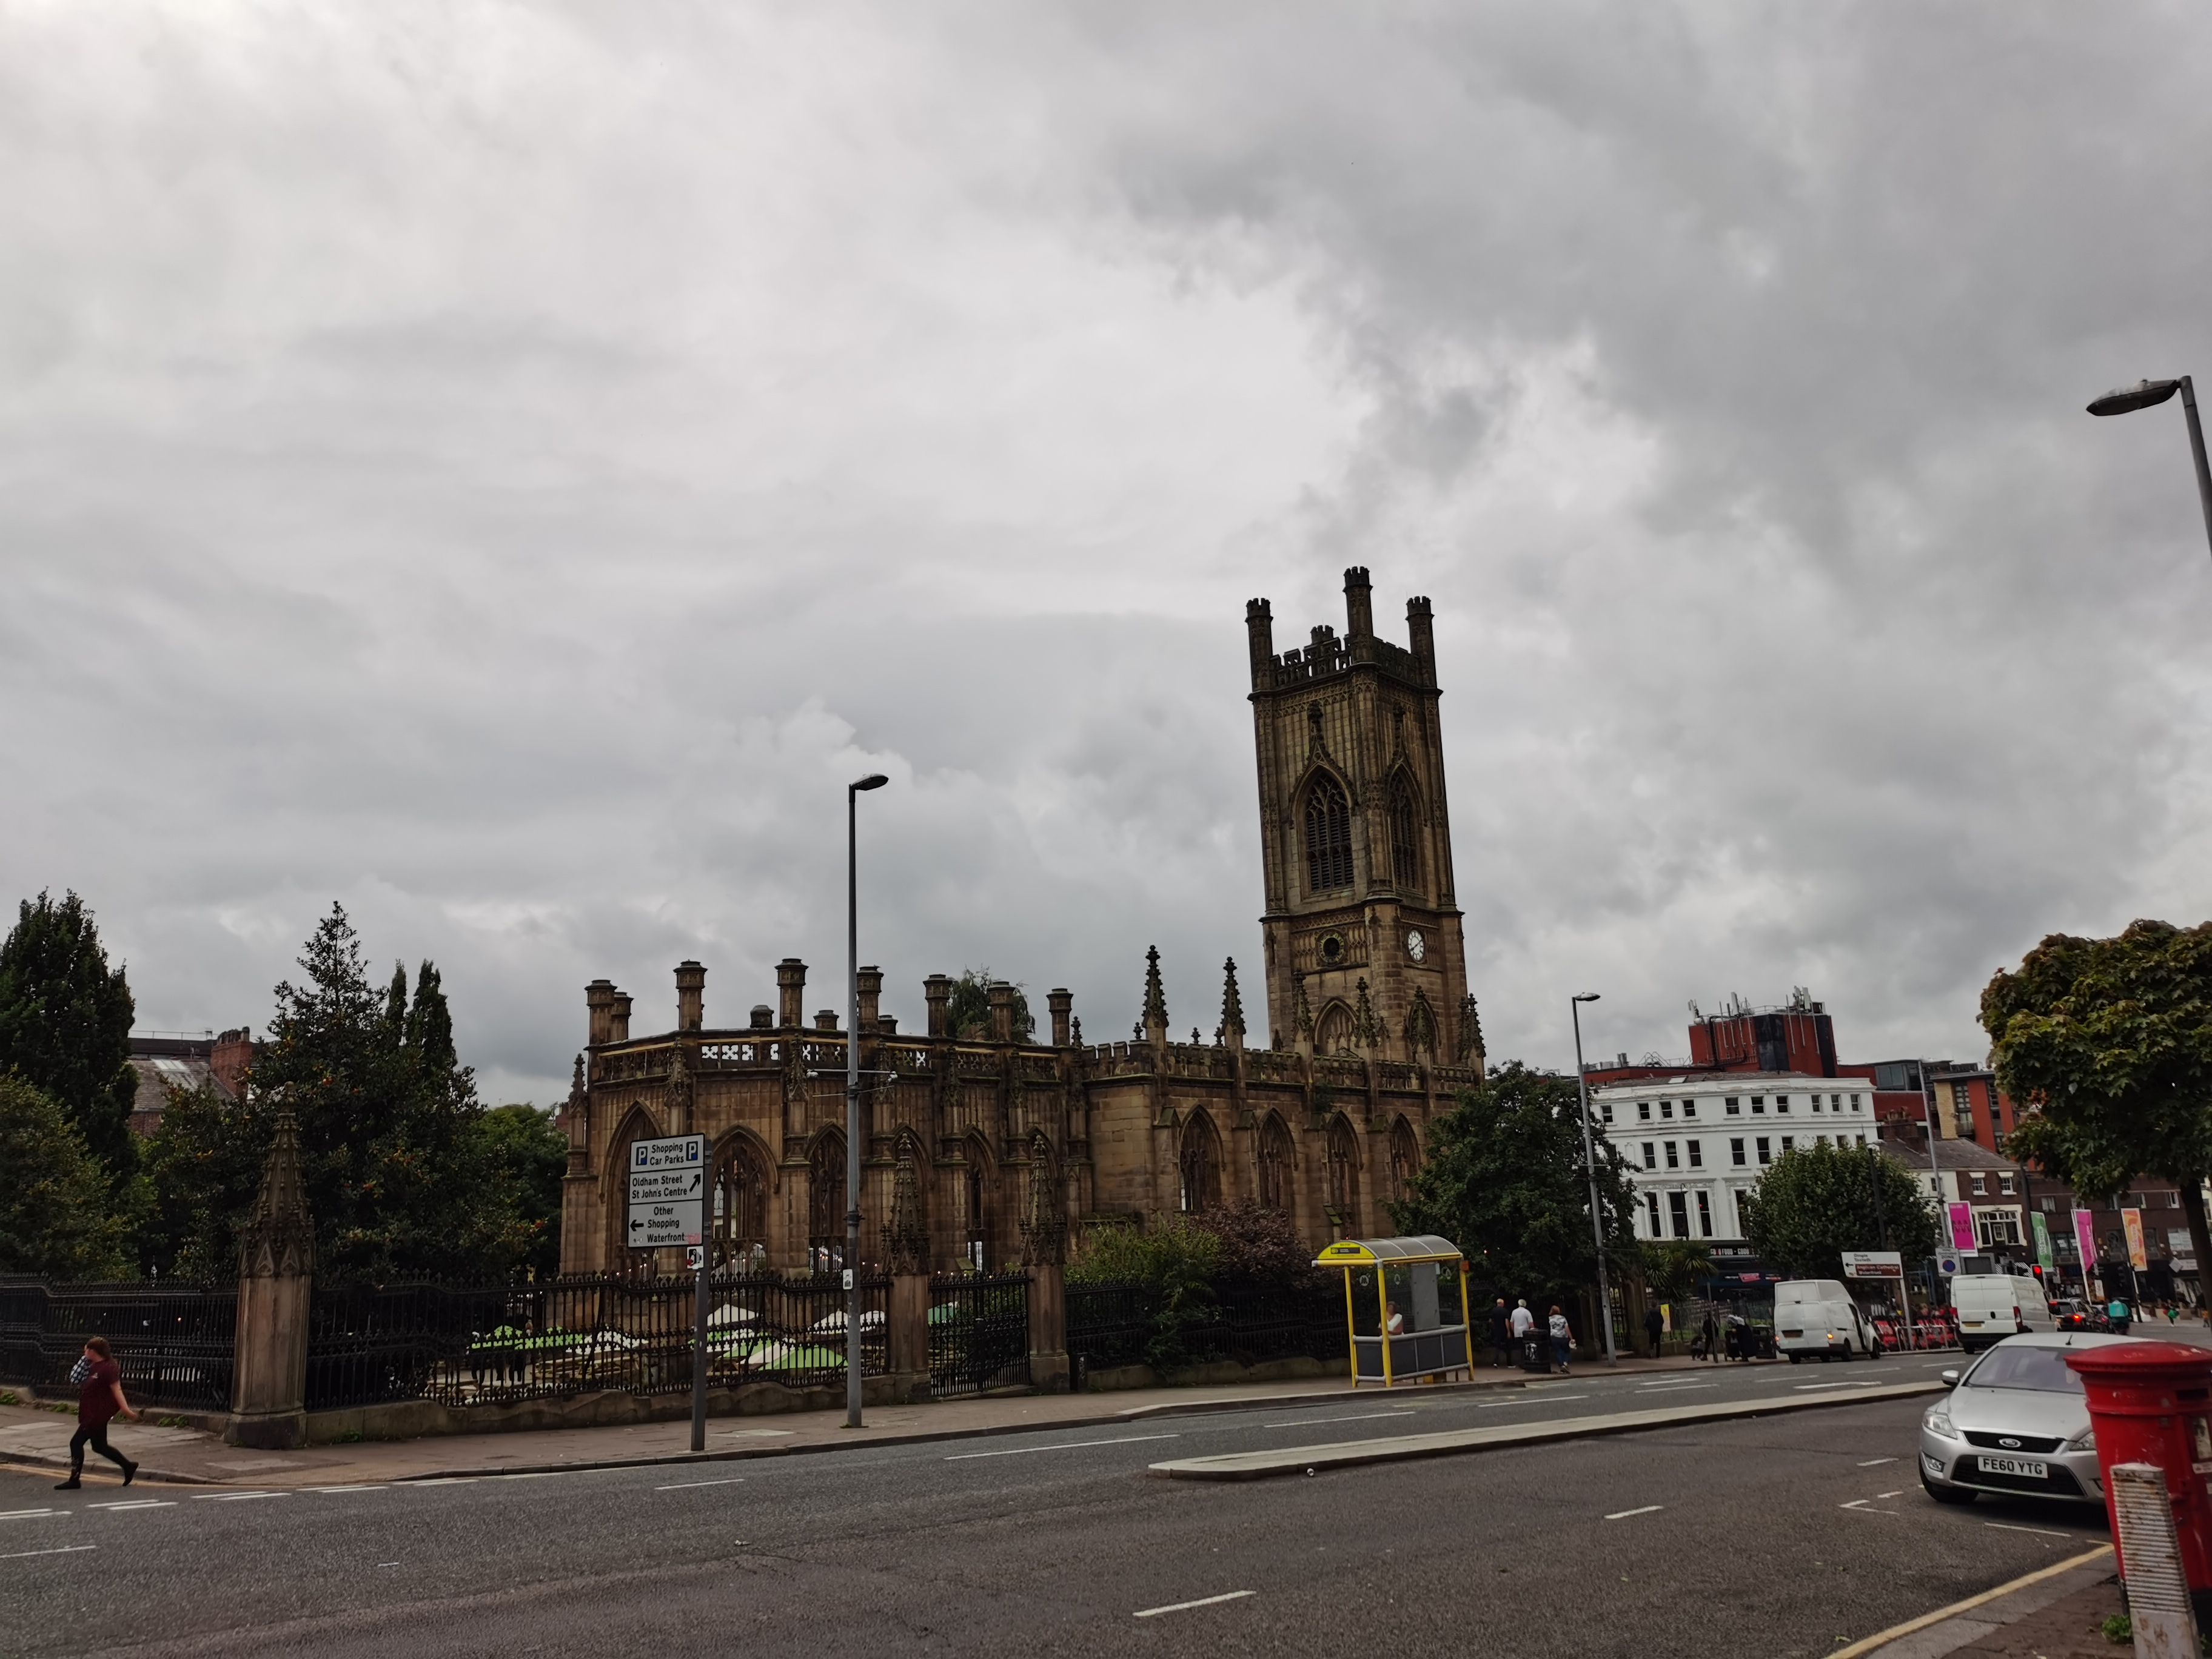
\includegraphics[width=\textwidth]{1Q.jpg}
\end{figure}

\begin{figure}[H]
    \centering
    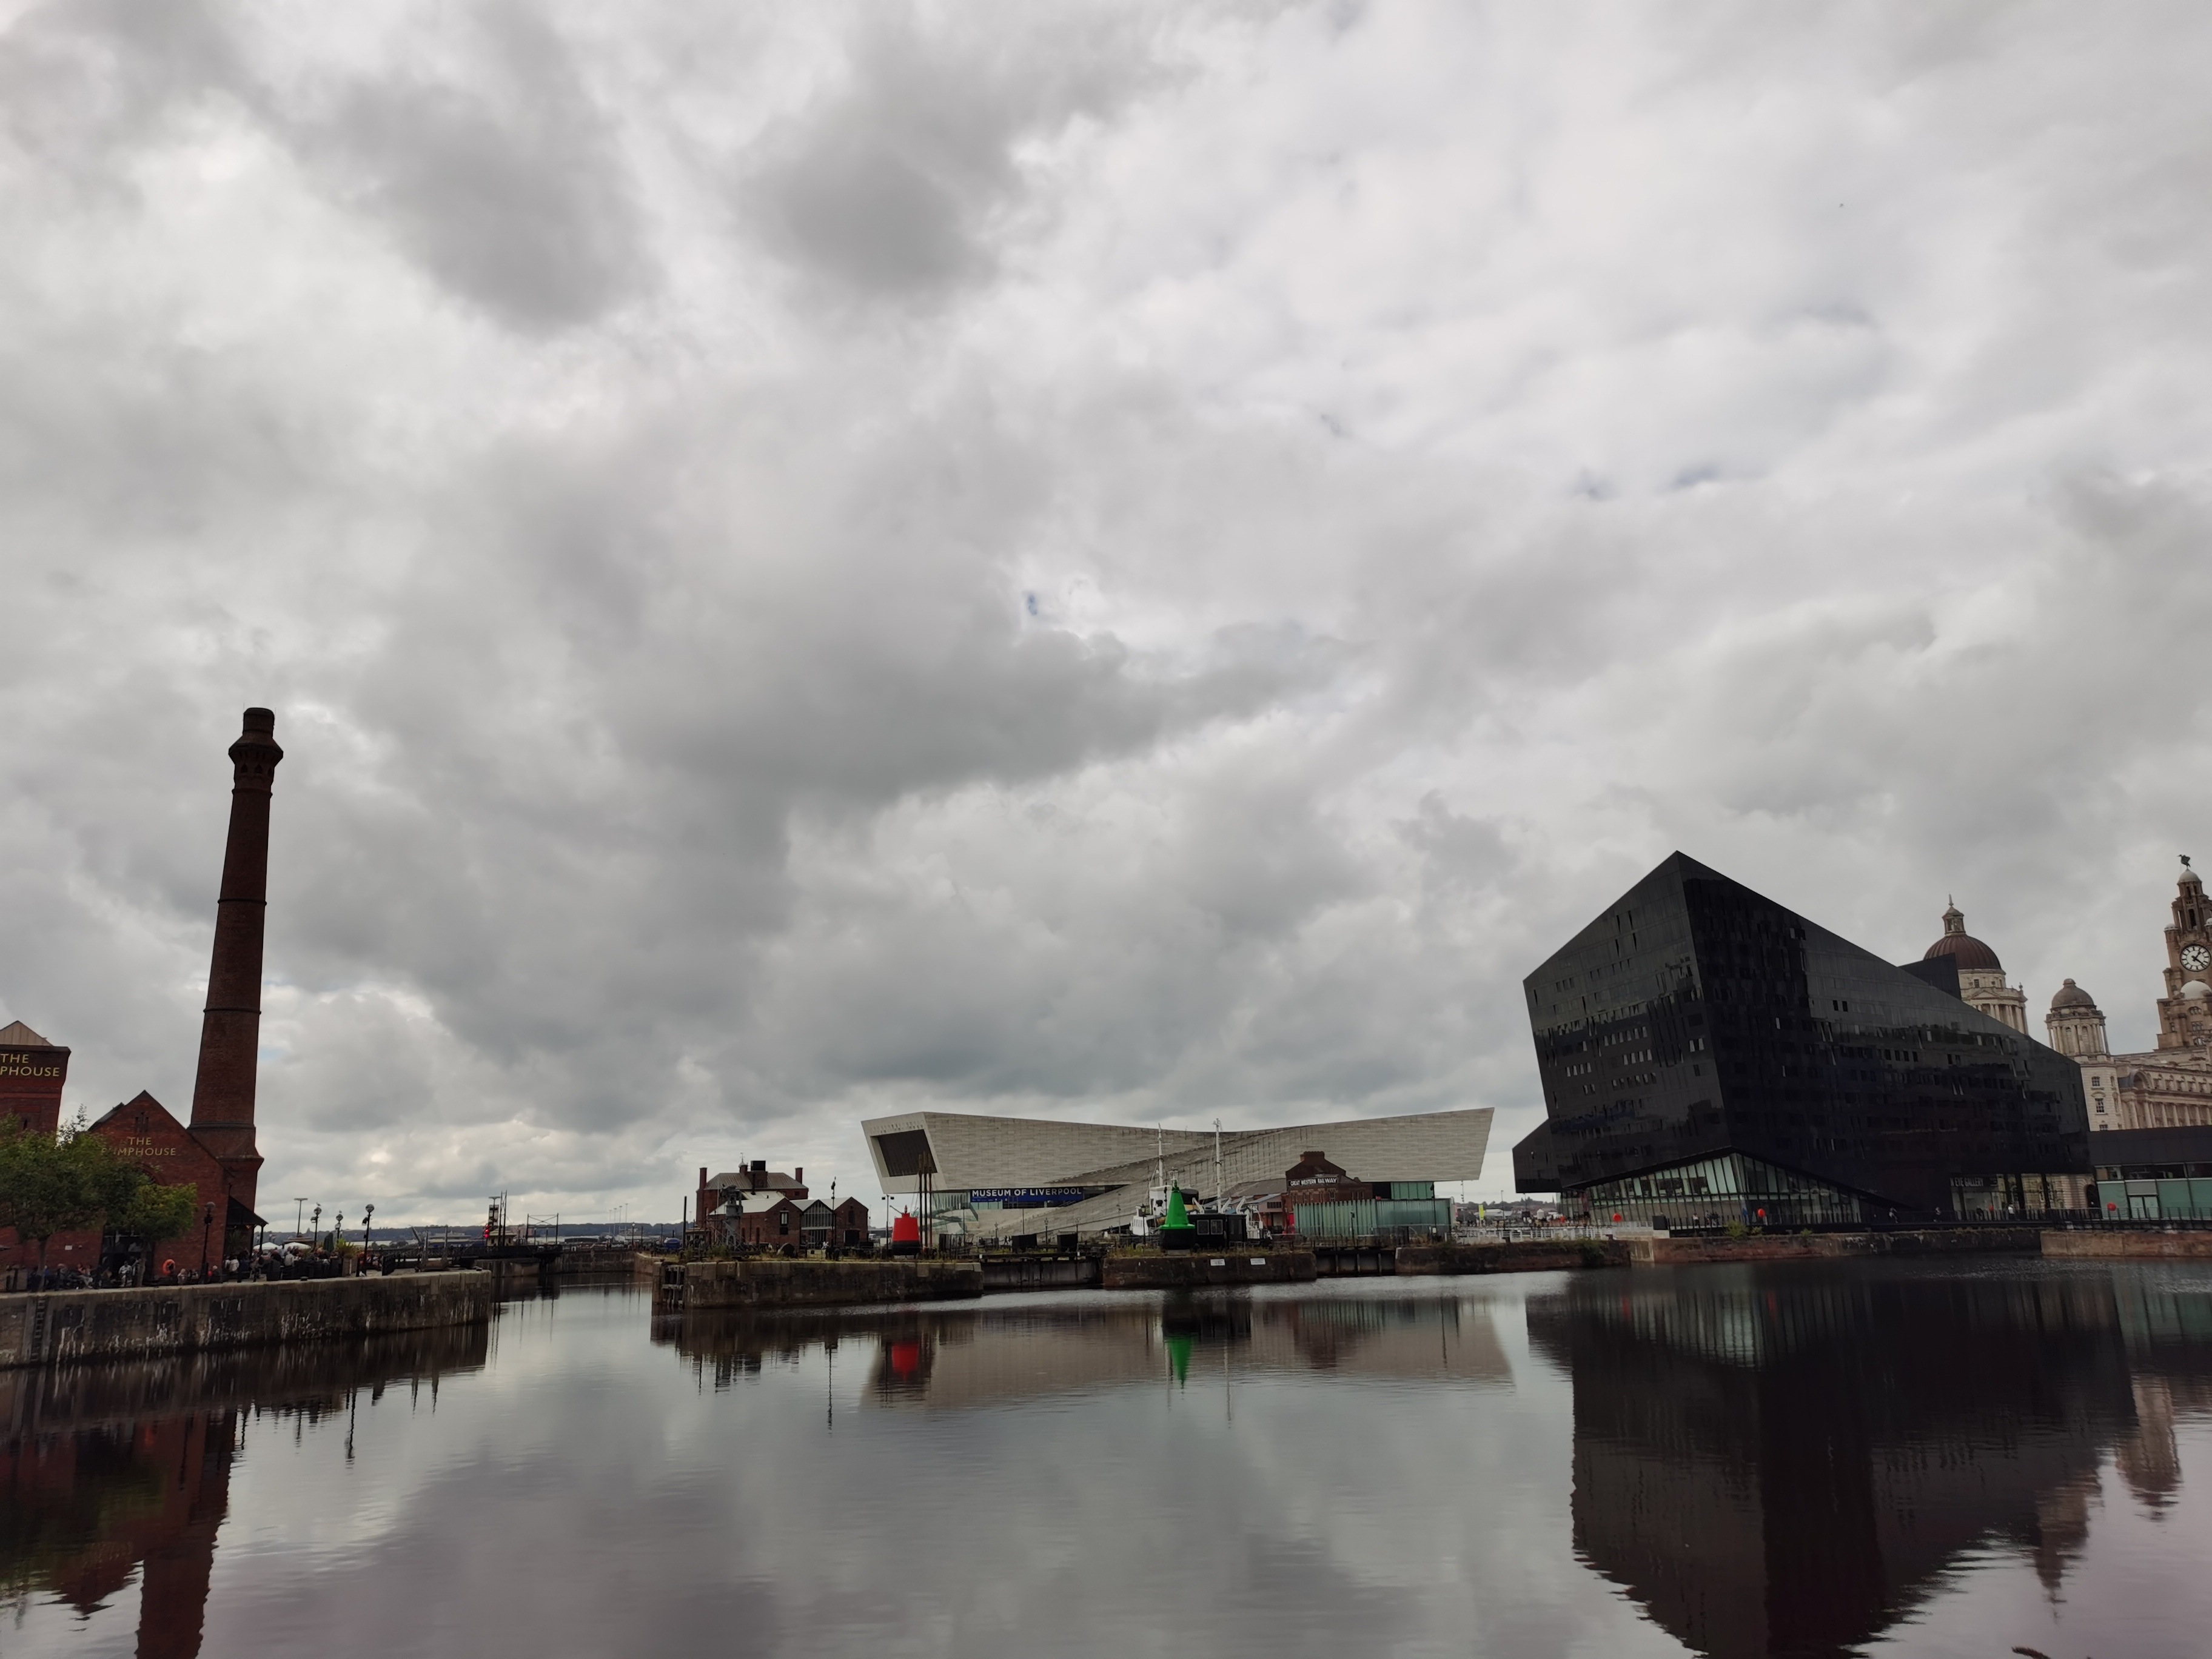
\includegraphics[width=\textwidth]{1R.jpg}
\end{figure}

\begin{figure}[H]
    \centering
    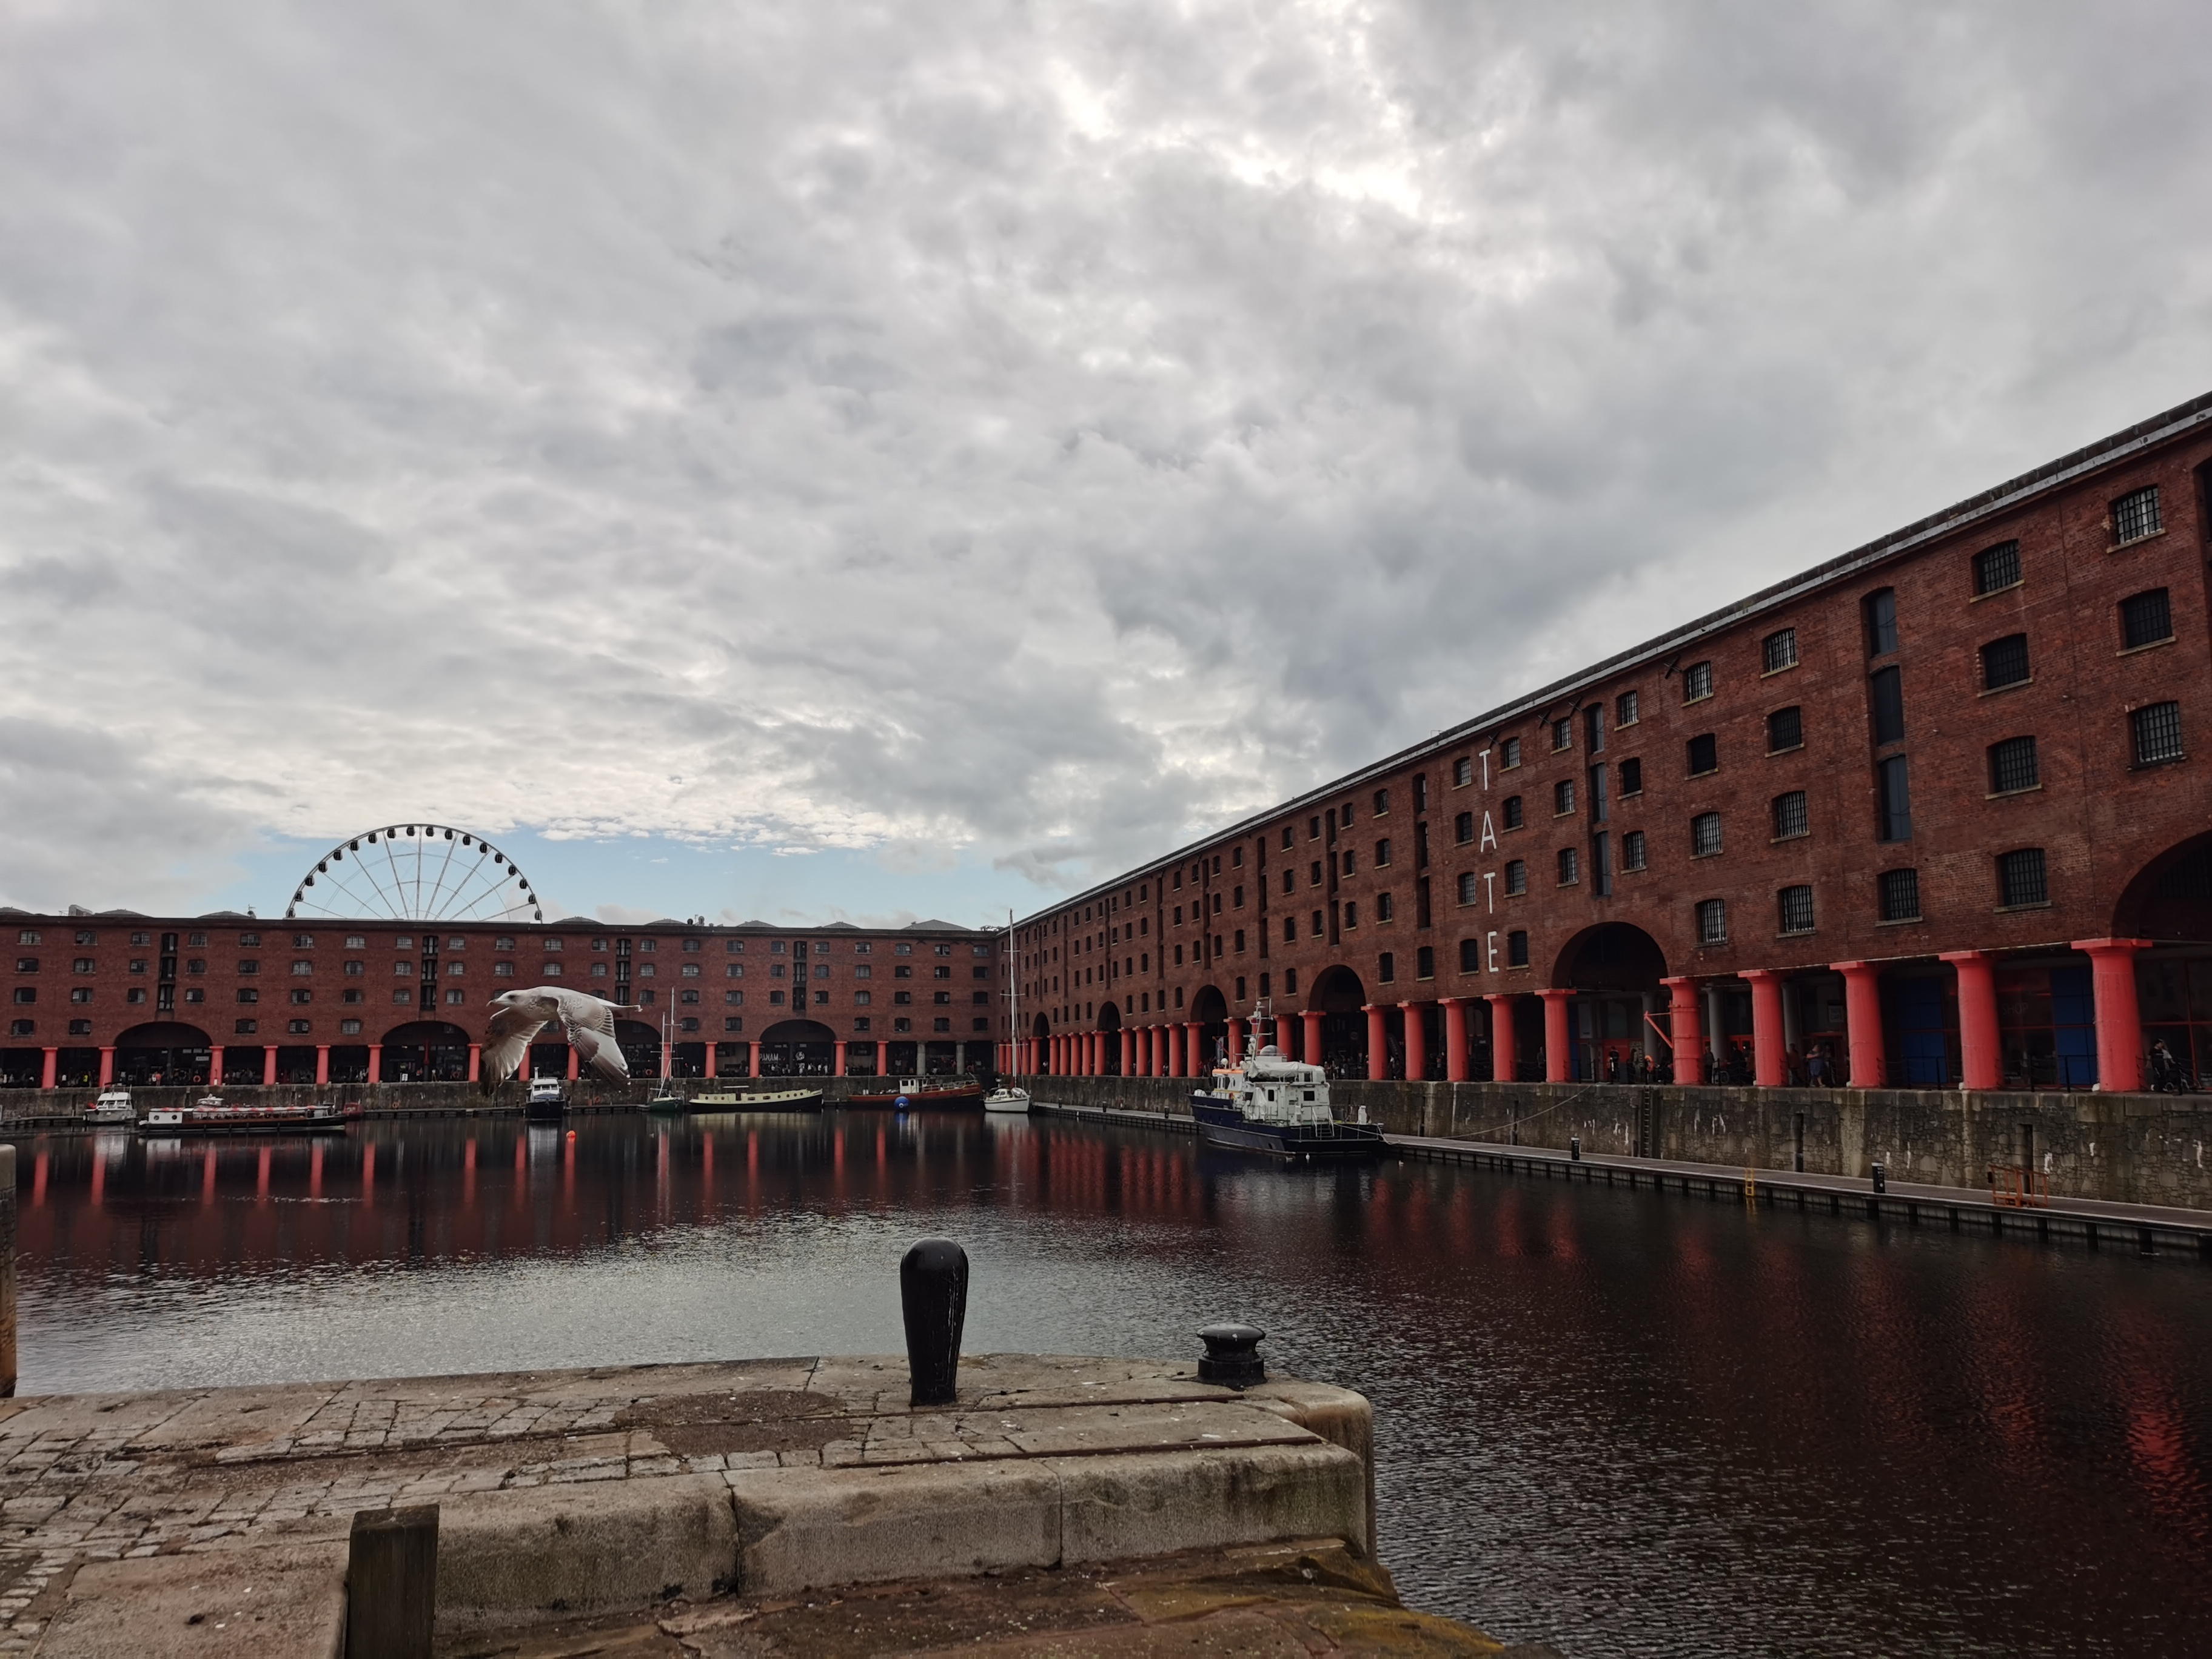
\includegraphics[width=\textwidth]{1S.jpg}
\end{figure}

\begin{figure}[H]
    \centering
    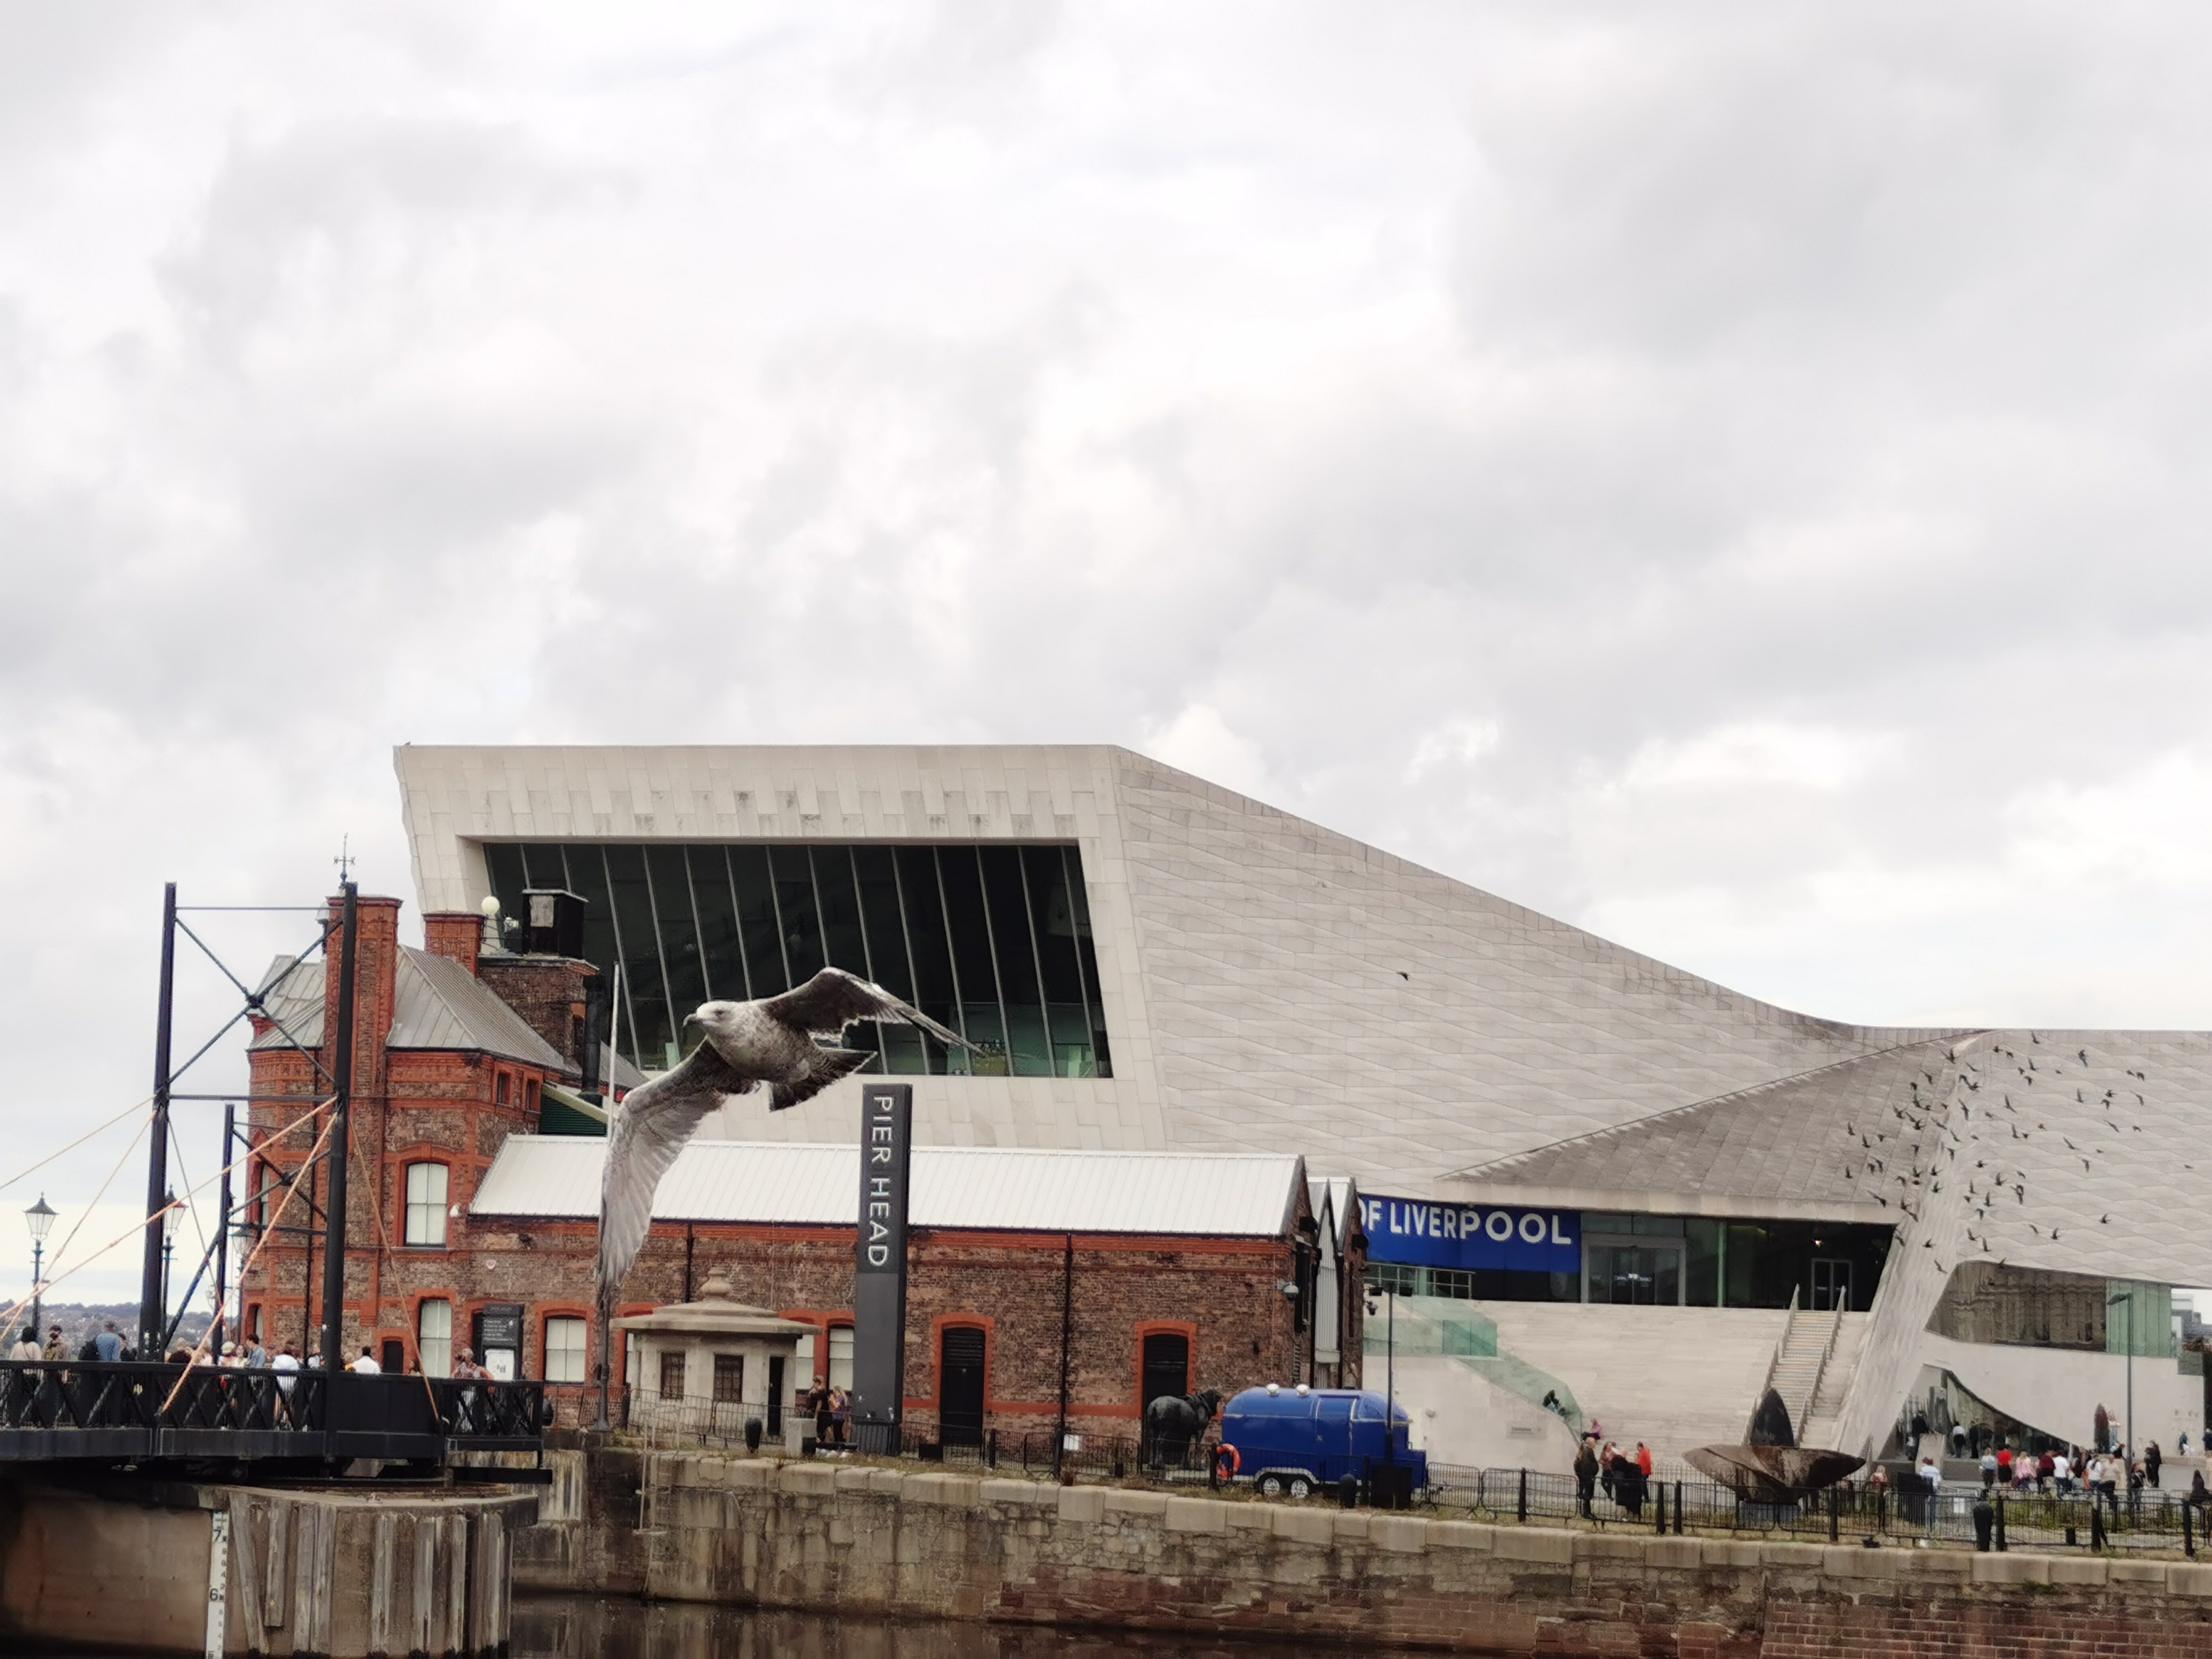
\includegraphics[width=\textwidth]{1T.jpg}
\end{figure}

\begin{figure}[H]
    \centering
    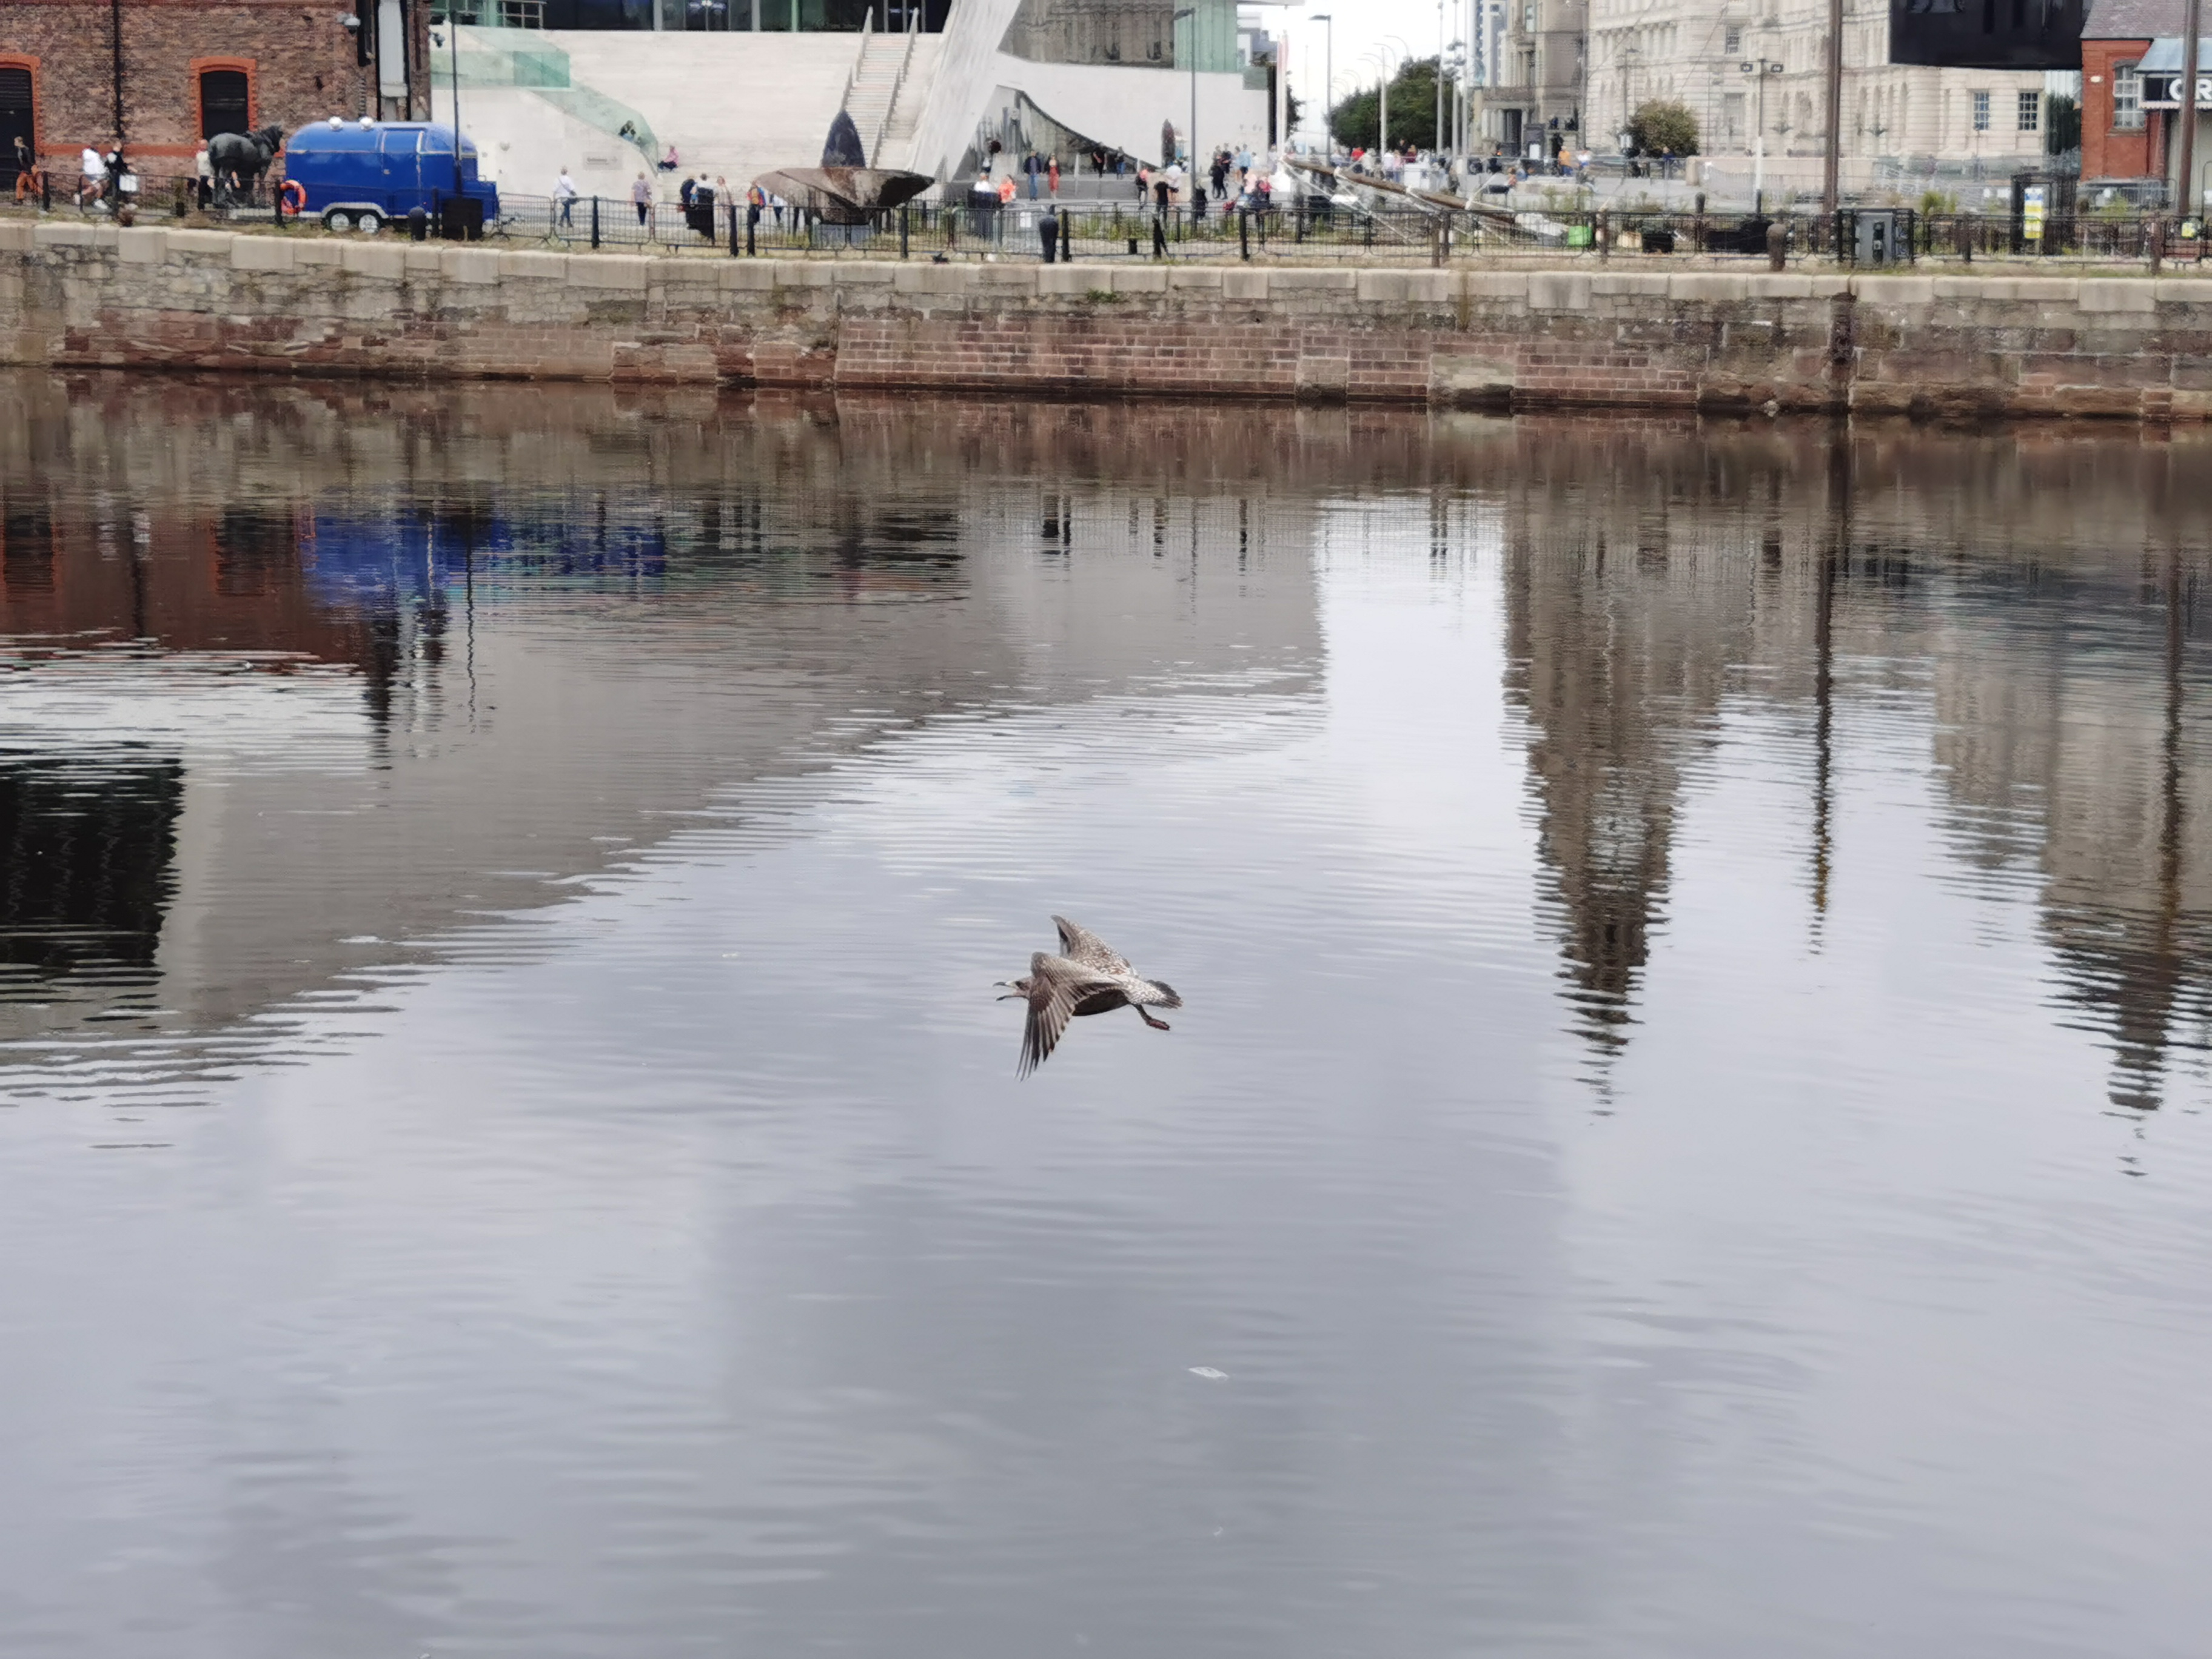
\includegraphics[width=\textwidth]{1U.jpg}
\end{figure}

\begin{figure}[H]
    \centering
    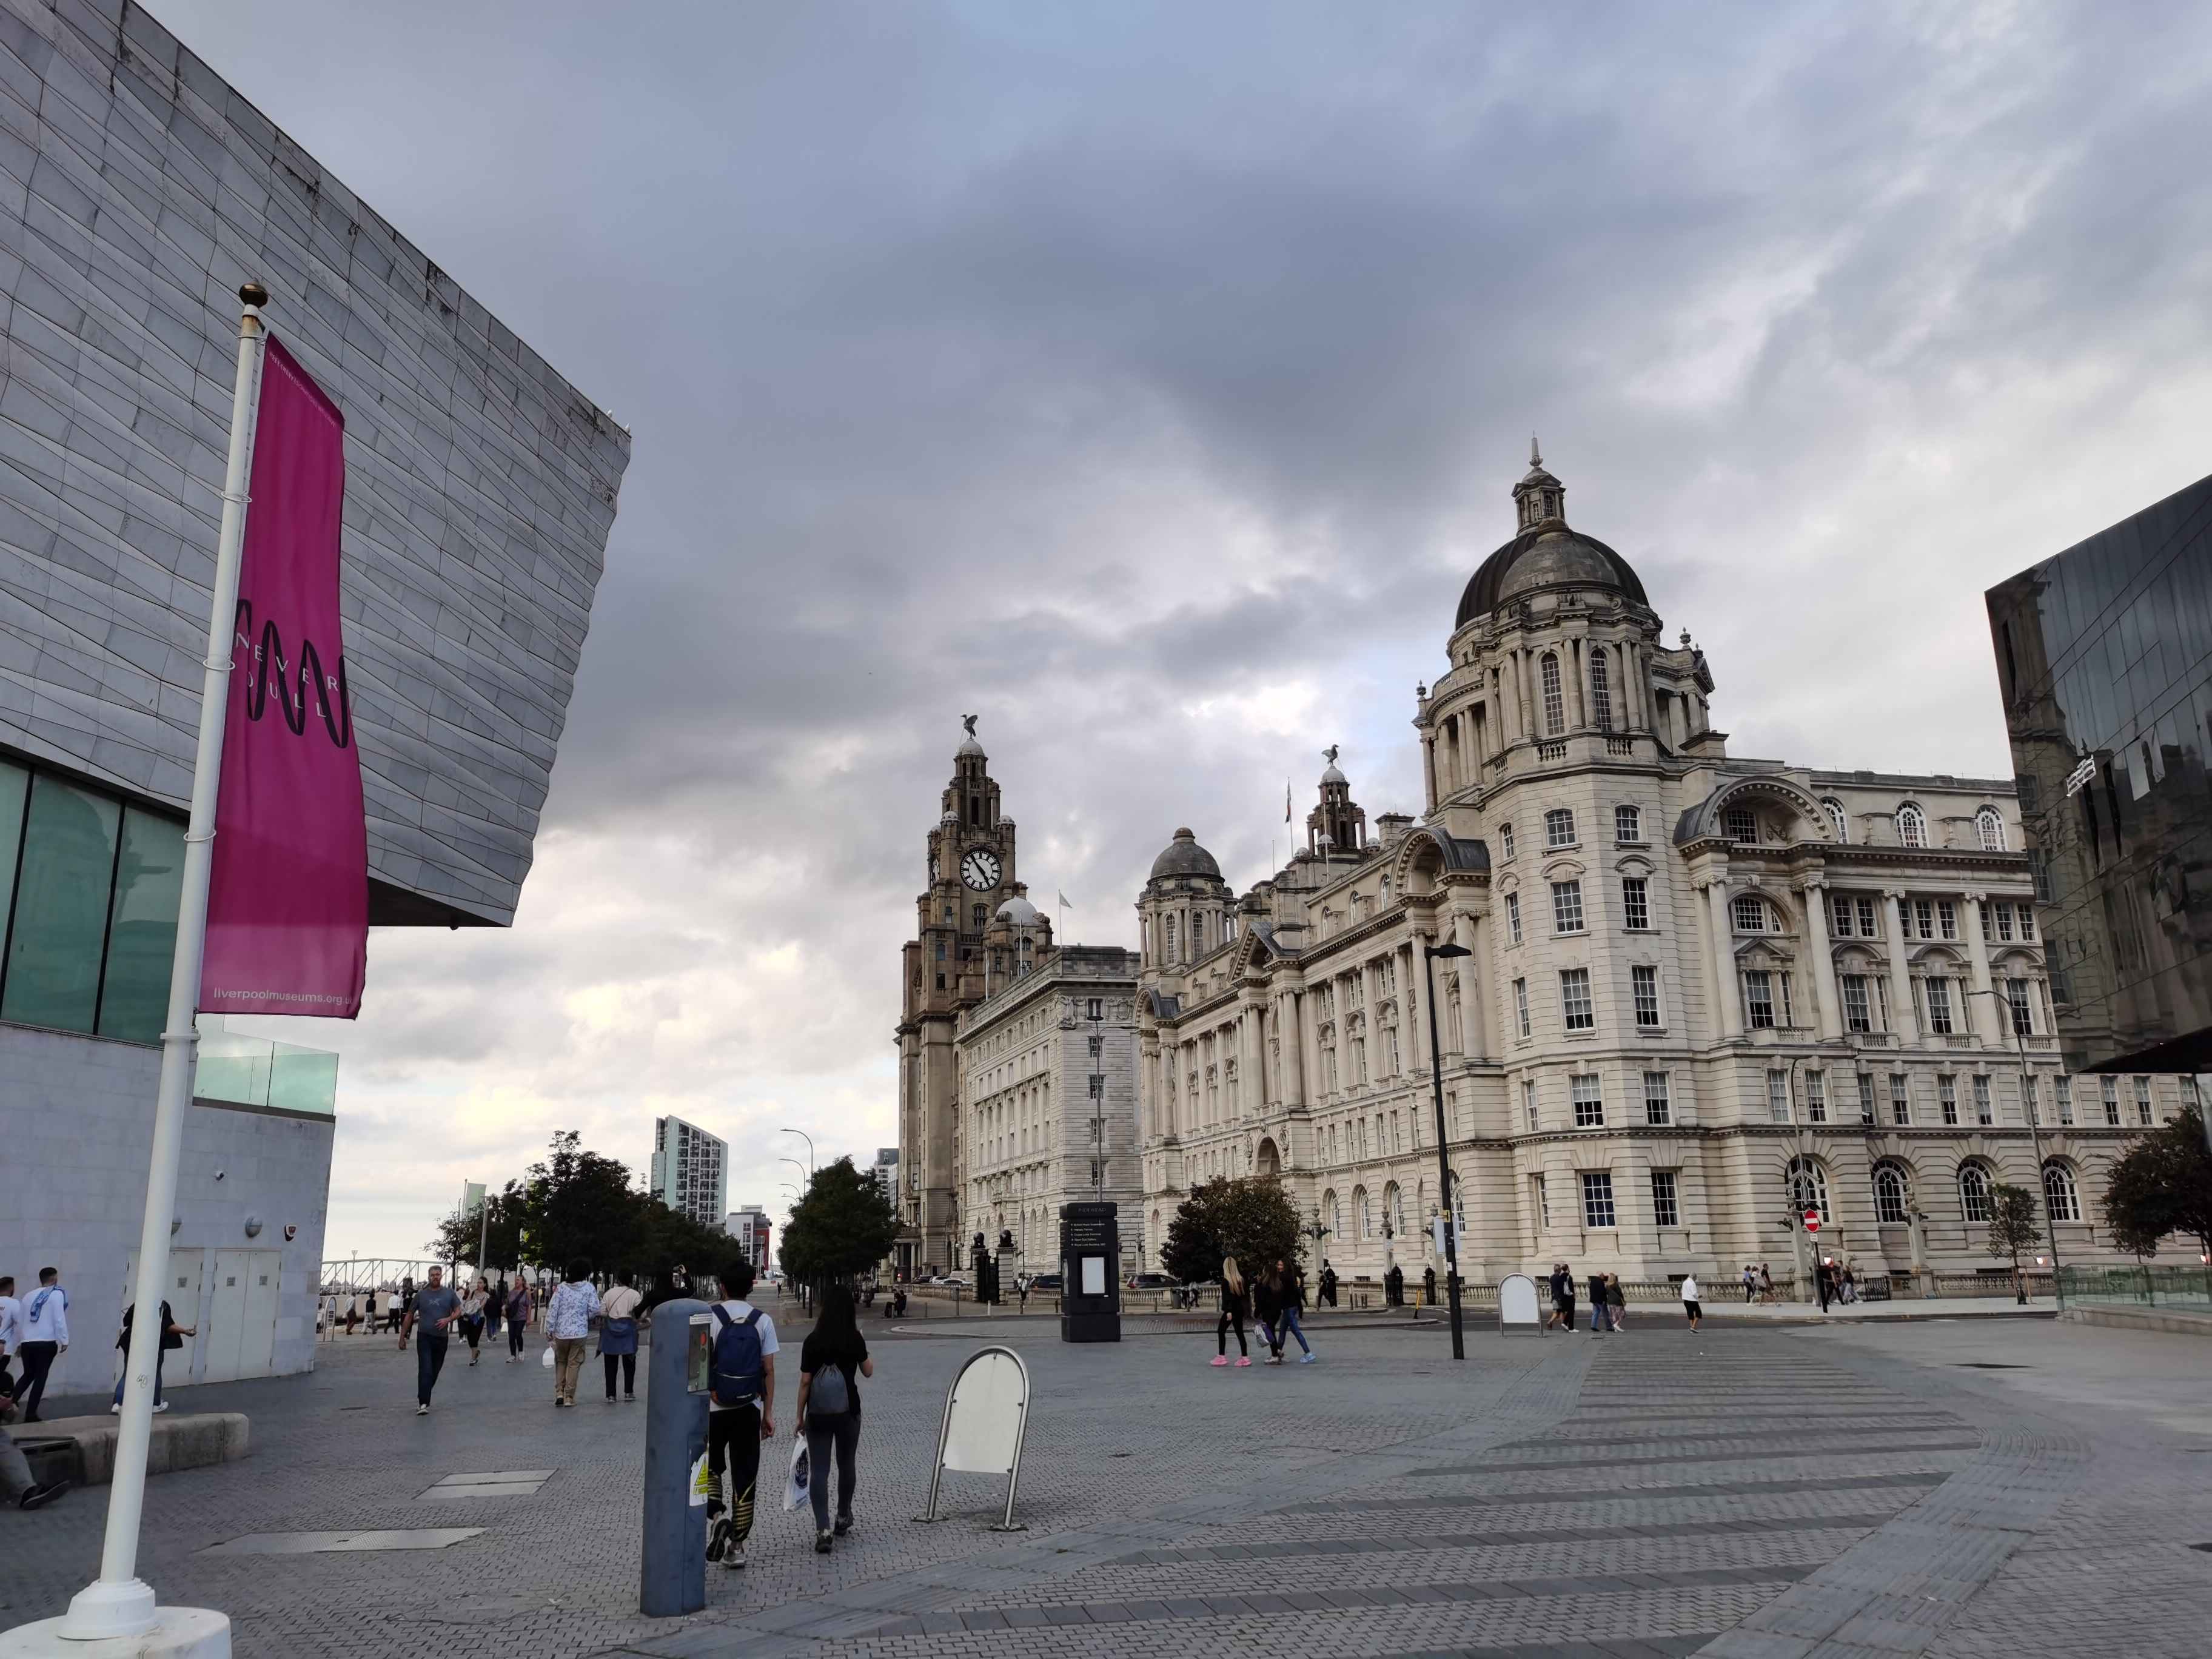
\includegraphics[width=\textwidth]{1V.jpg}
\end{figure}

\begin{figure}[H]
    \centering
    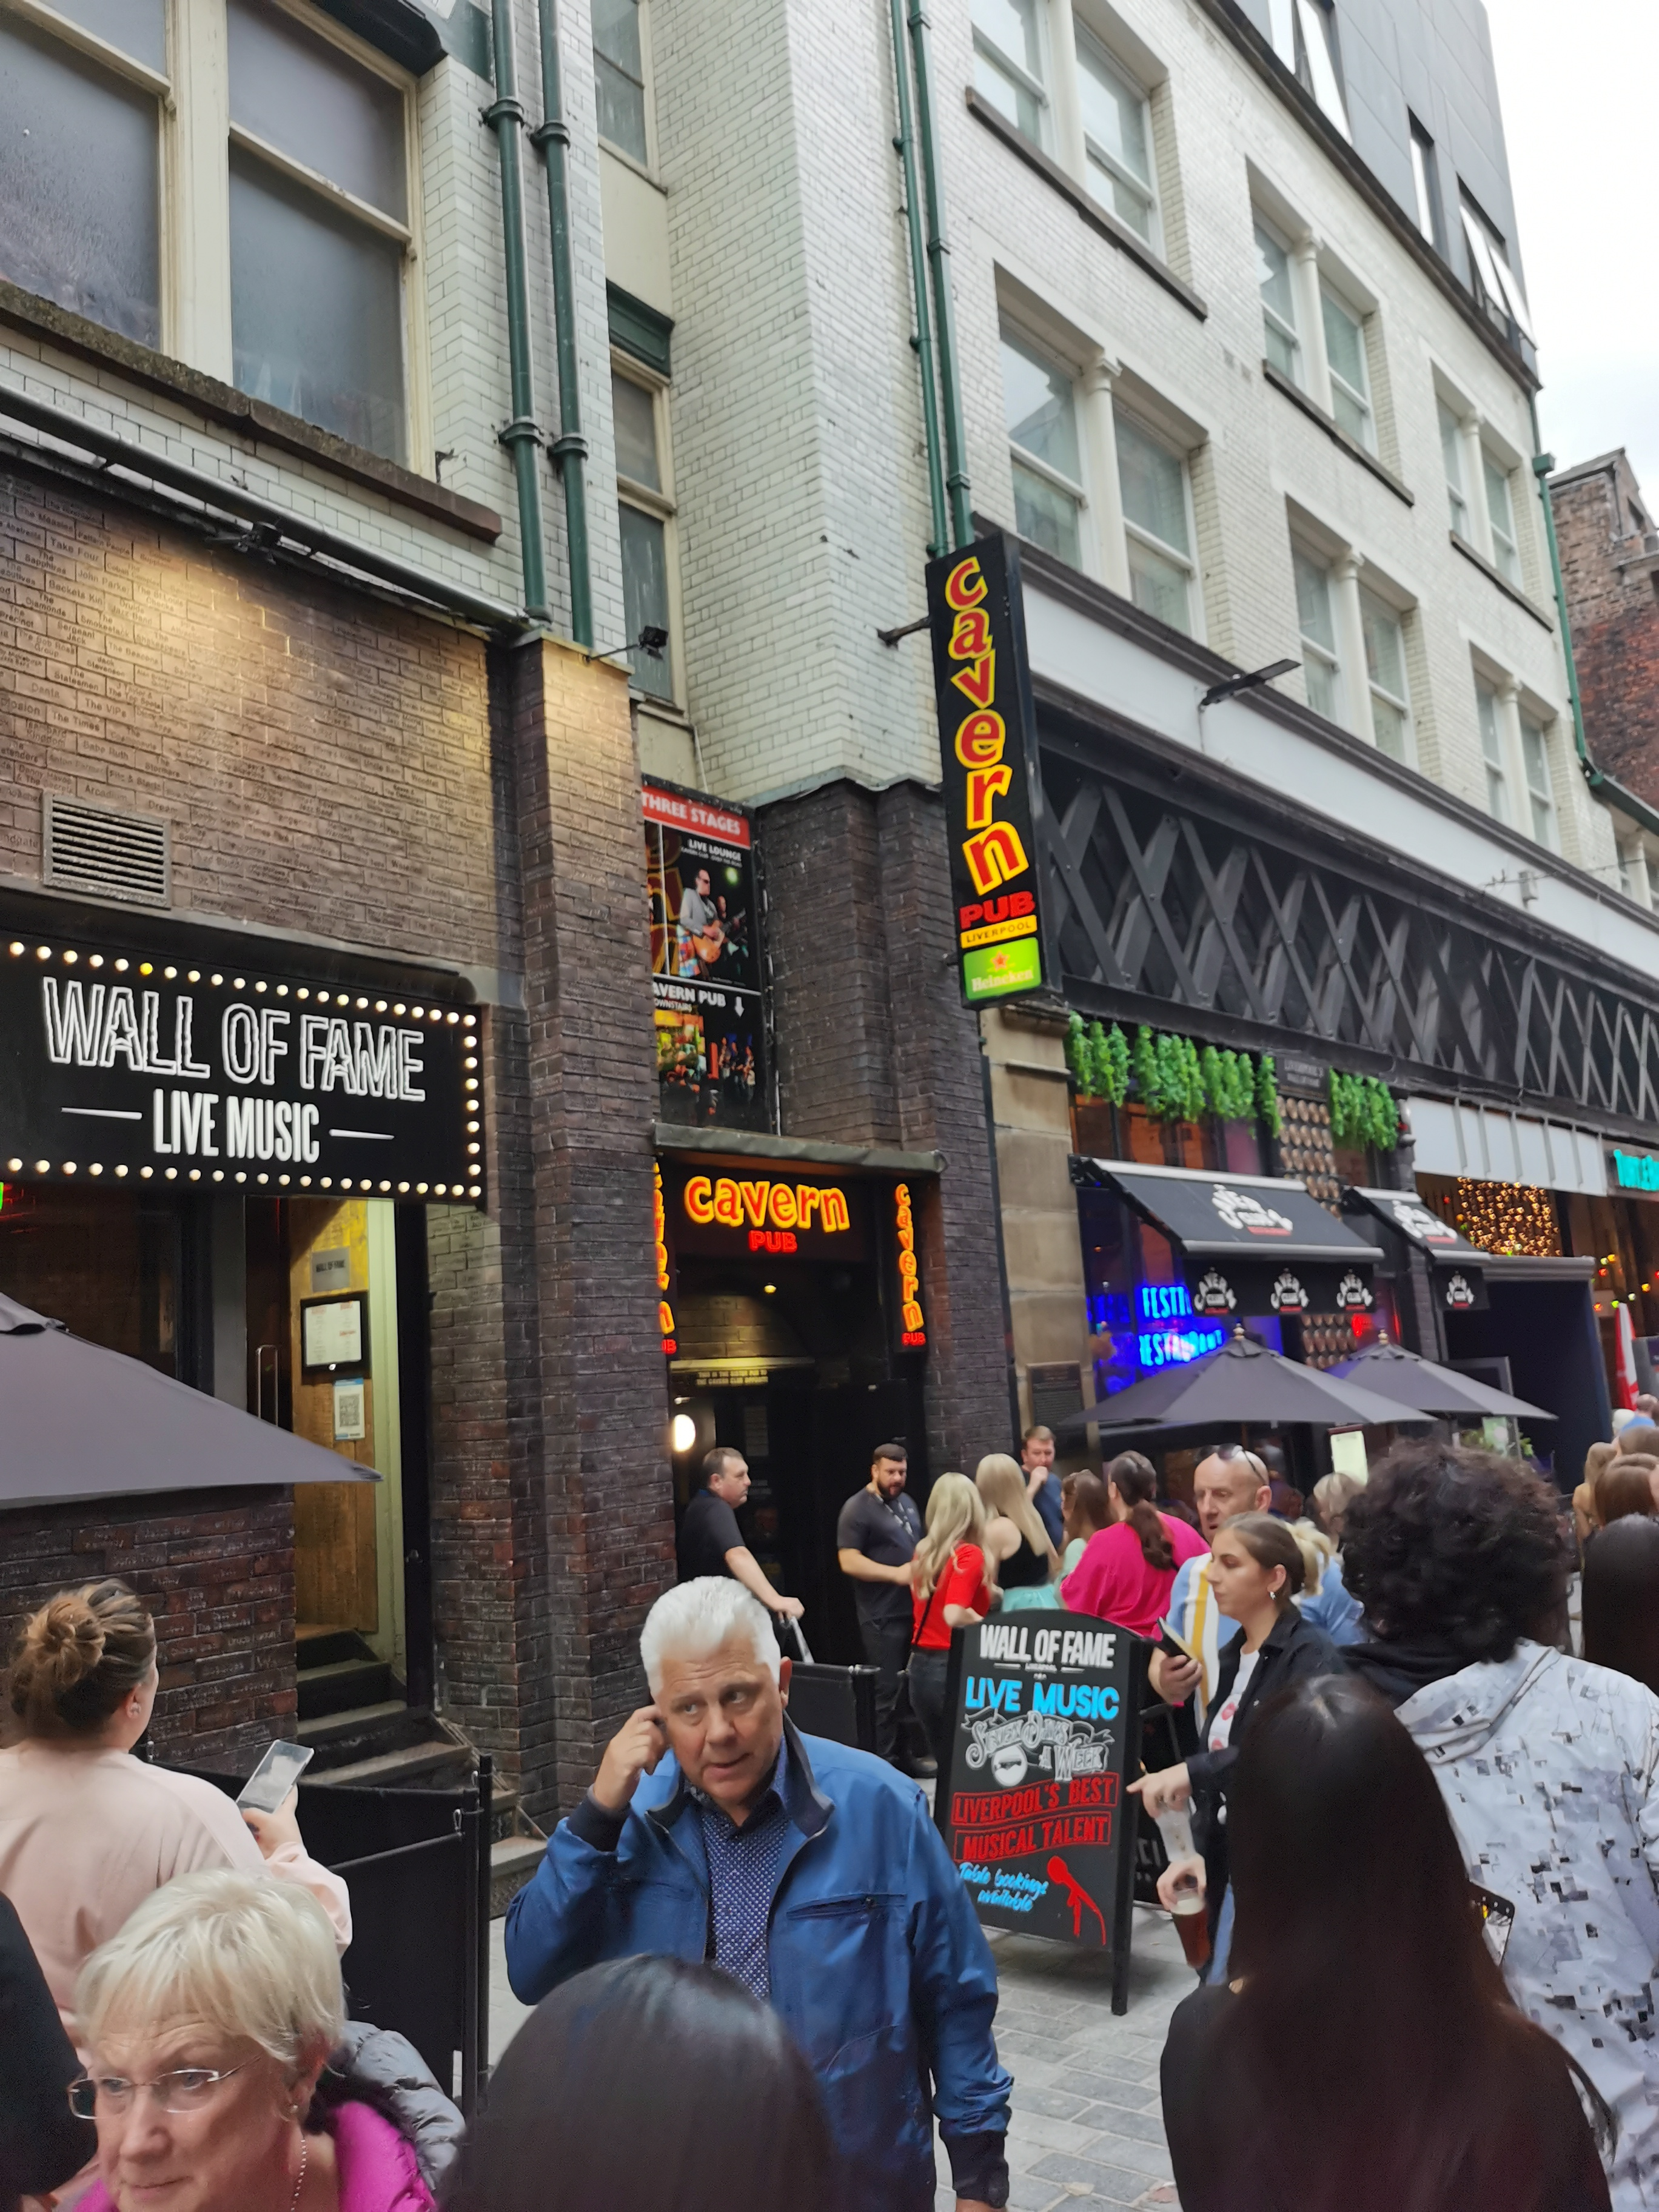
\includegraphics[width=\textwidth]{1W.jpg}
\end{figure}

\begin{figure}[H]
    \centering
    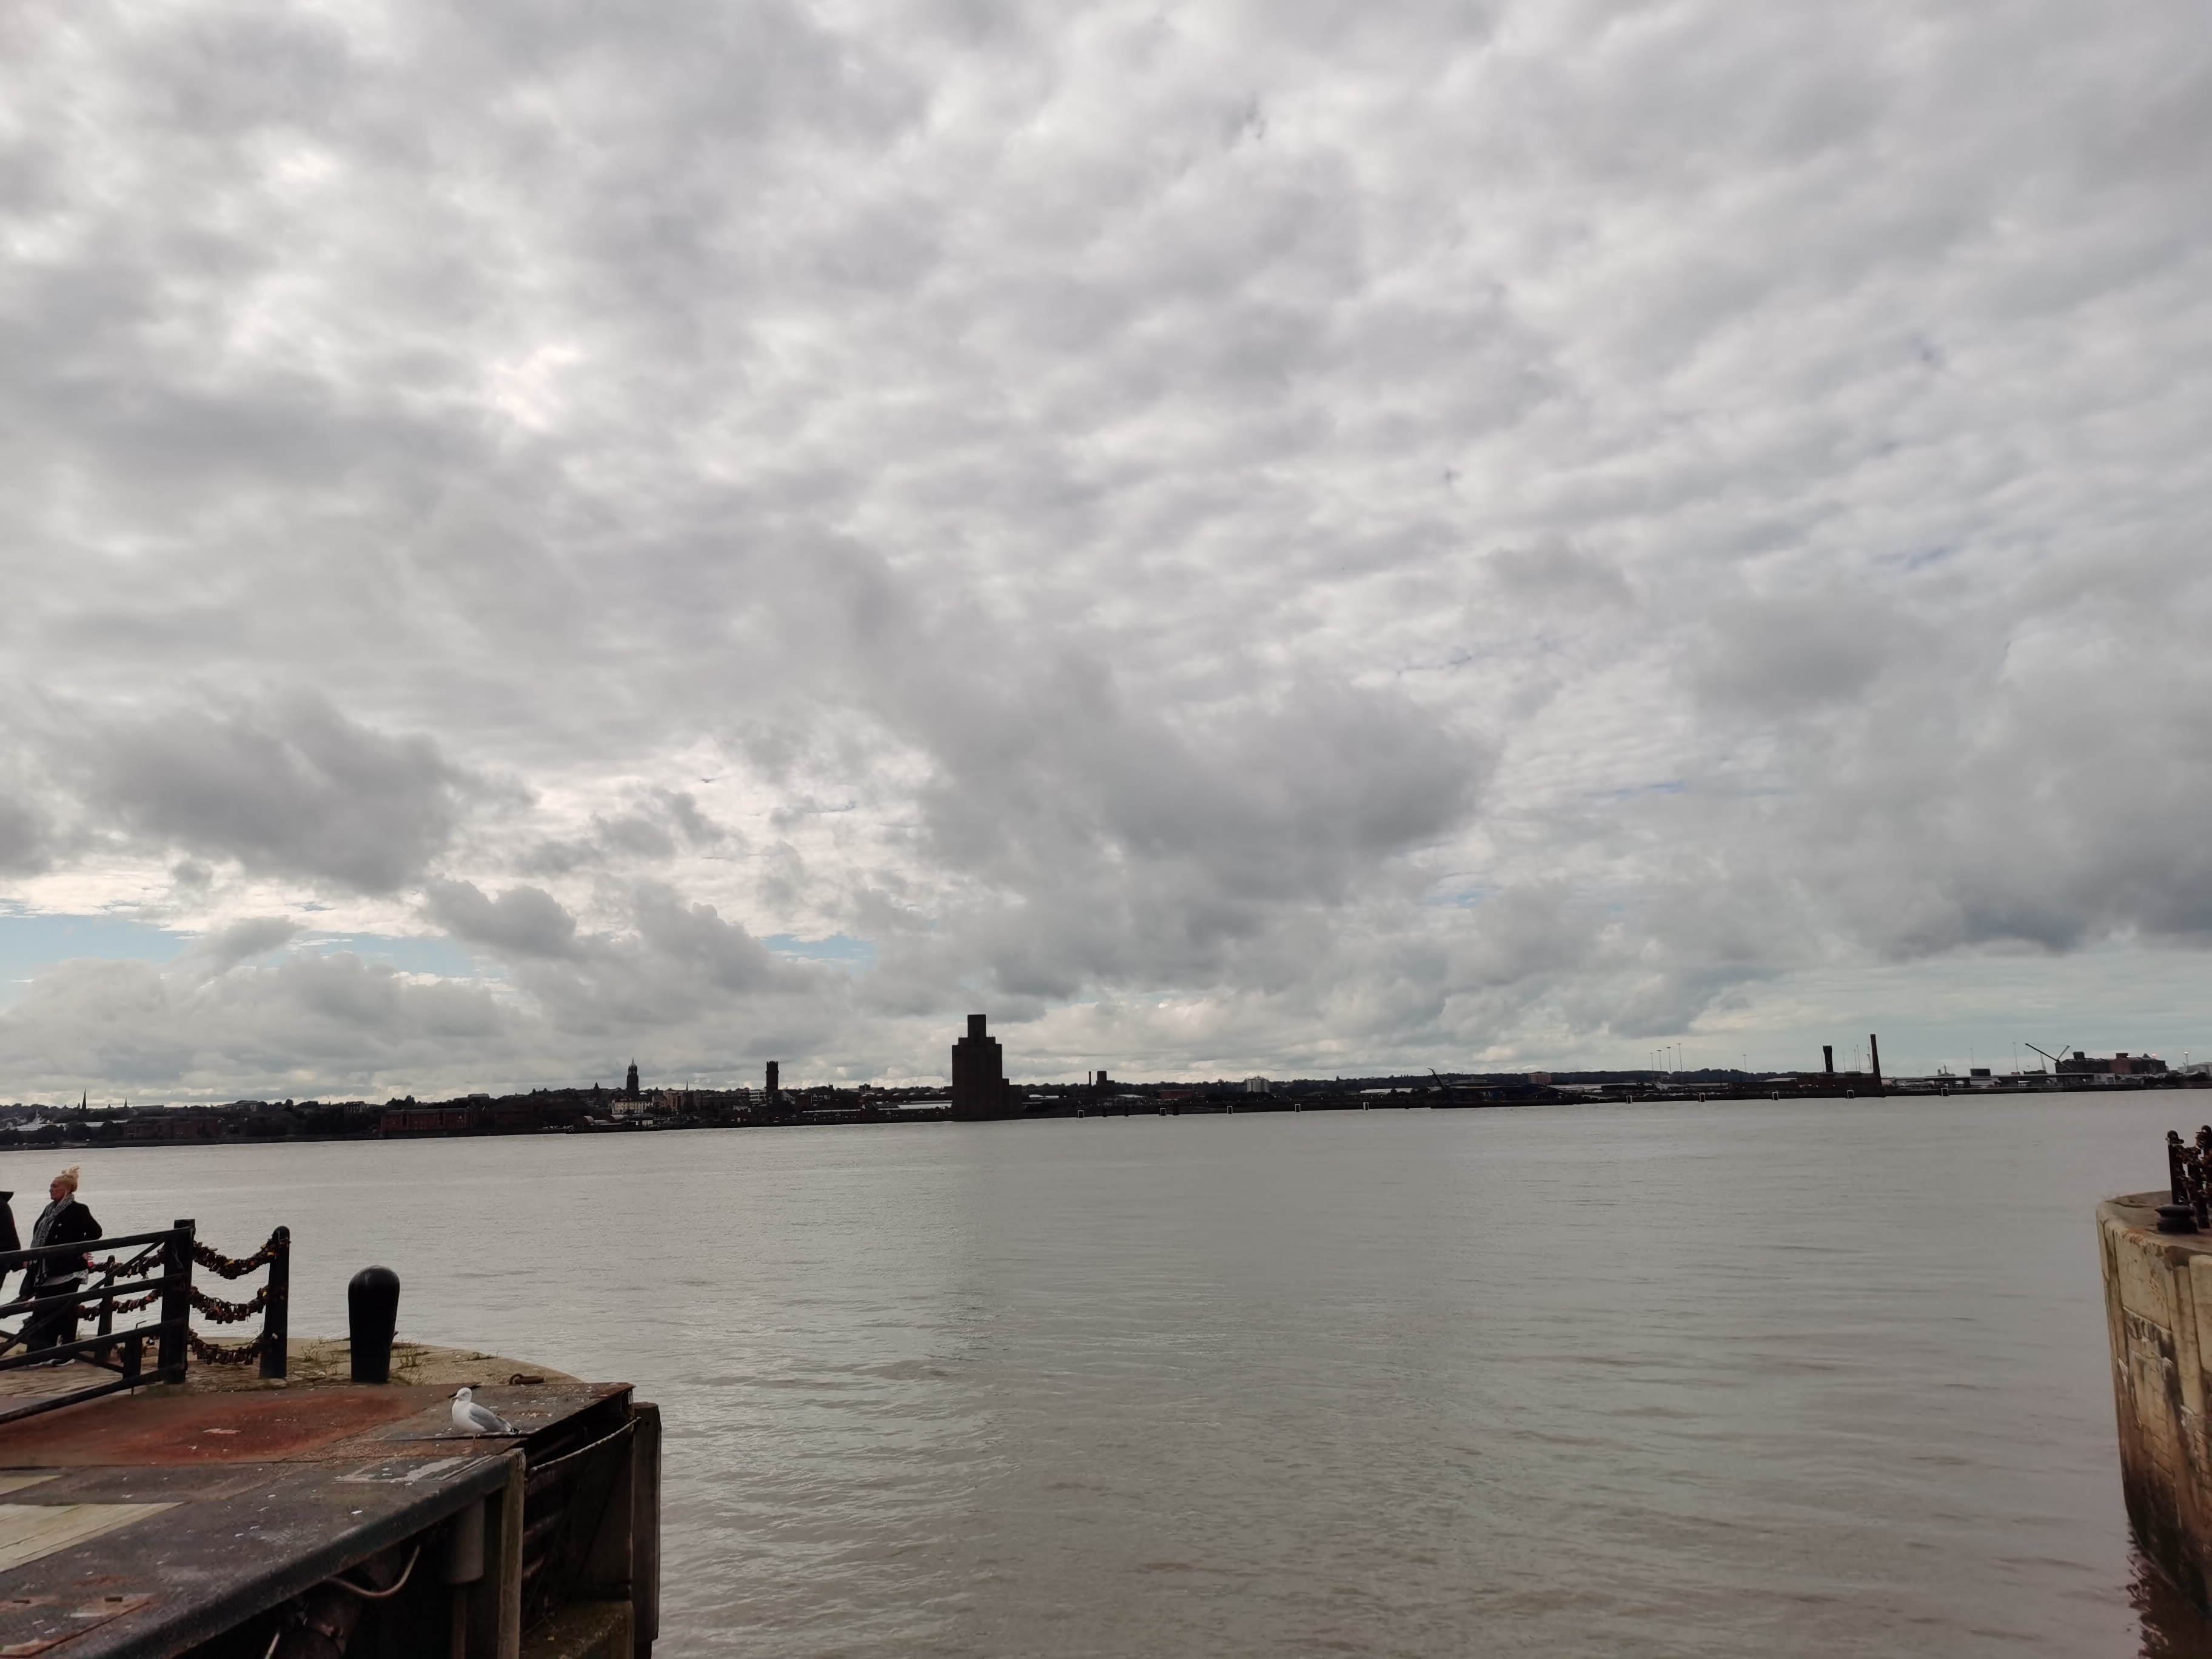
\includegraphics[width=\textwidth]{1X.jpg}
\end{figure}

\end{document}